% This is samplepaper.tex, a sample chapter demonstrating the
% LLNCS macro package for Springer Computer Science proceedings;
% Version 2.21 of 2022/01/12
%
\documentclass[runningheads]{llncs}
%
\usepackage[T1]{fontenc}
% T1 fonts will be used to generate the final print and online PDFs,
% so please use T1 fonts in your manuscript whenever possible.
% Other font encondings may result in incorrect characters.
%
\usepackage{subcaption}
\usepackage{amsmath}
\usepackage{comment}
\usepackage{graphicx}
\usepackage[table,xcdraw]{xcolor}
\usepackage{helvet,times,courier}
\usepackage{multirow}
\usepackage{algorithm2e}
\SetKwInput{KwParam}{Parameters}
\SetKw{KwFrom}{from}
\SetCommentSty{textit}

\usepackage{todonotes}

\usepackage{graphicx}
% Used for displaying a sample figure. If possible, figure files should
% be included in EPS format.
%
% If you use the hyperref package, please uncomment the following two lines
% to display URLs in blue roman font according to Springer's eBook style:
%\usepackage{color}
%\renewcommand\UrlFont{\color{blue}\rmfamily}
%\urlstyle{rm}
%
\sloppy
\hyphenation{make-span}

\renewcommand{\topfraction}{1}
\renewcommand{\bottomfraction}{1}
\renewcommand{\textfraction}{-0.1}

\begin{document}
%
\title{Swarm Intelligence-Driven Dispatching Rules for Semiconductor Production
}
%
\titlerunning{Swarm Intelligence-Driven Dispatching Rules for Semiconductor Production}
% If the paper title is too long for the running head, you can set
% an abbreviated paper title here
%
\author{Ramsha~Ali\inst{1}\orcidID{0000-0002-4794-6560} \and
Peyman~Eftekhari\inst{1}\orcidID{0009-0007-4198-392X} \and
Martin~Gebser\inst{1}\orcidID{0000-0002-8010-4752} \and
Stephan~Leitner\inst{2}\orcidID{0000-0001-6790-4651} \and
Gerhard~Friedrich\inst{1}\orcidID{0000-0002-1992-4049}
}
%
\authorrunning{R. Author et al.}
% First names are abbreviated in the running head.
% If there are more than two authors, 'et al.' is used.
%
\institute{Department of Artificial Intelligence and Cybersecurity \and
	Department of Management Control and Strategic Management \\ University of Klagenfurt, Austria \\
	\email{\{ramsha.ali,peyman.eftekhari,martin.gebser, \\ stephan.leitner,gerhard.friedrich\}@aau.at}} % \\
%	\url{https://www.aau.at}}

%
\maketitle              % typeset the header of the contribution
%
\begin{abstract}
The immense complexity of semiconductor production
% , characterized by high-volume, low-mix and low-volume, high-mix environments,
demands for advanced dispatching strategies that transcend traditional rule-based systems. This paper introduces a novel approach to dispatching rules derived from Swarm Intelligence (SI) techniques, specifically designed to tackle the intricate dynamics of large-scale semiconductor manufacturing processes. Our approach integrates simulation and optimization methods to investigate and enhance operational efficiency, addressing both the scalability of schedules and their practical implementation. We employ a customizable simulation framework to model a semiconductor manufacturing environment, wherein various dispatching rules % , including FIFO, CR, RANDOM,
as well as our proposed SI-driven method are assessed.
% The core of our approach lies in its ability to adaptively configure scheduling priorities based on real-time production dynamics, thus significantly improving the responsiveness and throughput of manufacturing processes.
The effectiveness of these dispatching rules is quantitatively evaluated through a series of simulations that measure key performance indicators such as Work in Progress (WIP) levels, throughput, and operational variability across different production scenarios.
This study not only elucidates the potential of SI techniques in refining production dispatching strategies, but also provides a simulation-based evaluation framework that can assist in the further development of intelligent dispatching systems. 

\keywords{Swarm intelligence \and Ant colony optimization \and Greedy search \and Semiconductor production \and Scheduling \and Dispatching \and Simulation}
\end{abstract}
%
%
%
\section{Introduction}
\label{sec:introduction}
%As the digital transformation deepens across various sectors, the demand for more powerful, energy-efficient, and smaller semiconductors continues to escalate. This surge in demand places immense pressure on semiconductor manufacturers to scale up production without compromising quality. Semiconductor production involves hundreds of sophisticated steps, each of which must be precisely controlled to ensure the functionality and yield of the final product \cite{kopp2020smt2020}. The complexity is exacerbated by the rapid pace of innovation in semiconductor design, which frequently shifts production parameters and process requirements.

Dispatching and scheduling are critical in semiconductor manufacturing because they directly impact the throughput and utilization of resources. Dispatching refers to the process of assigning work to specific machines in real-time, while scheduling involves pre-planning the sequence and timing of operations to optimize certain objectives, such as minimizing the total completion time or balancing the load across different machines~\cite{schumann2022scheduling}.

For smaller volumes at workcenters in the semiconductor fab, which can be modeled as flexible job shops, optimal solutions can be achieved using mathematical optimization \cite{waschneck2018deep}. However, in larger and more dynamic environments, the complexity and computational time constraints limit the feasibility of applying mathematical optimization. Consequently, optimization is typically implemented on a local scale, isolated to individual workcenters. In complex scenarios, this localized approach to production scheduling may lead to solutions that are globally sub-optimal.

Dispatching involves determining which job should be performed at which time, by which resource. This decision is based on the availability of resources and the urgency of job orders \cite{Hopp2011}. However, as production scenarios become more complex, particularly in high-tech industries such as semiconductor manufacturing, the static nature of traditional dispatching rules often proves insufficient. These rules typically do not account for the rapid changes in production conditions or the intricate dependencies between different production processes.  
Traditional dispatching solutions often fall short in such an environment, as they cannot adequately adapt to the dynamic and complex nature of semiconductor production. This inadequacy can lead to sub-optimal decisions that compromise operational efficiency \cite{Uzsoy1992}.

The complexity of scheduling in large-scale semiconductor production, a cornerstone of operational management, is significantly influenced by the unpredictable nature of processing times and machine availabilities. Variability in processing times can arise from differences in equipment performance, material handling durations, or the unique characteristics of each set of wafers, while frequent machine breakdowns can cause substantial disruptions, underscoring the need for strong and adaptable scheduling strategies \cite{leachman1996benchmarking}. Scheduling involves meticulously planning and organizing production activities to ensure optimal resource utilization and synchronized product flows across various manufacturing stages, which is crucial not only for maintaining high throughput but also for minimizing makespan \cite{schumann2022scheduling}. The task is particularly daunting in semiconductor manufacturing due to the high variability in production processes, the sensitive nature of the materials, and stringent quality requirements \cite{May2006}. Each semiconductor product may pass through hundreds of processing steps, requiring precise timing and coordination. The complexity is further compounded by the need to accommodate a high mix of product types, each with distinct processing needs and priorities, and to integrate new product introductions seamlessly into the production schedule without disrupting ongoing operations \cite{Moench2011}.

In this paper, we explore the complexities of scheduling within large-scale Semiconductor Manufacturing Scheduling Problems (SMSP), commonly referred to as fabs. Fabs are intricate production settings distinguished by their specialized job flows and advanced machinery. Modern semiconductor fabs manage the processing of tens of thousands of operations daily across over 1000 different machines \cite{kopp2020smt2020}. These machines are grouped by functionality—such as diffusion, etching, or metrology—and each step in the manufacturing process can be assigned to any machine that offers the necessary capabilities. The scheduling challenge in semiconductor production thus involves assigning specific operations to appropriate machines and determining the optimal sequence of these operations on each machine. Additionally, schedules must be flexible and capable of rapid adjustments in response to machine failures or deviations in the process.

In our previous work \cite{Ali2024}, we proposed a Greedy Search based Ant Colony Optimization (GSACO)
algorithm for (re-)scheduling semiconductor production operations. 
Our algorithm harnesses Ant Colony Optimization (ACO) \cite{Dorigo2019} for exploration, while
Greedy Search (GS) \cite{Papadimitriou} enables responses in short time. 
In this way, GSACO overcomes limitations of a state-of-the-art Constraint Programming approach \cite{Perron2023}
on large-scale SMSP instances. Our approach synergistically combines probabilistic operation sequencing with a greedy machine assignment strategy, targeting up to five operations per lot with the primary objective of minimizing makespan. Building on this foundational work, the current paper extends these initial concepts by proposing an enhanced algorithm, GSACO-I, specifically designed to optimize operational throughput in addition to minimizing makespan. This development marks a significant advancement in our methodology, aiming to refine the dispatching rules further though simulation.

The paper is organized as follows. 
Section~\ref{sec:lit_rev} provides literature review.
In Section~\ref{sec:problem_f}, we formulate SMSP in terms of the well-known flexible job shop scheduling problem (FJSSP). 
% and Section \ref{sec:aco} describes the overview of the ACO approach. 
Our GSACO-I algorithm is presented in Section~\ref{sec:gsaco}.
In Section~\ref{sec:sim} we present the customized simulation adopted from \cite{Kovacs2022}.
Section~\ref{sec:results} provides and discusses experimental results.
Finally, Section~\ref{sec:conclusion} concludes the paper.


%The complexity of scheduling is intensified by the unpredictable nature of processing times and machine availabilities. Variability in processing times may arise from differences in equipment performance, material handling durations, or the unique characteristics of each set of wafers. Furthermore, frequent machine breakdowns can lead to substantial disruptions, underscoring the need for strong and adaptable scheduling strategies \cite{leachman1996benchmarking}.

%Scheduling in large-scale semiconductor production is a cornerstone of operational management that directly influences the effectiveness and efficiency of the entire manufacturing process \cite{schumann2022scheduling}. It involves planning and organizing production activities to ensure that resources are utilized optimally and product flows are synchronized across various stages of the manufacturing process. Effective scheduling is critical not only for maintaining high throughput but also for minimizing makespan.

%The scheduling of semiconductor manufacturing is notably complex due to the high variability in production processes, the sensitive nature of the materials involved, and the stringent quality requirements \cite{May2006}. Each semiconductor product may pass through hundreds of processing steps, requiring precise timing and coordination. Moreover, the high mix of product types, each with different processing needs and priorities, adds another layer of complexity \cite{Mönch2011}. This complexity is further exacerbated by the need to integrate new product introductions seamlessly into the production schedule without disrupting ongoing operations.

%Scheduling production operations within the intricate landscape of semiconductor manufacturing represents one of the most daunting challenges in resource allocation. The dynamic nature of manufacturing environments—characterized by unpredictable fluctuations in process and demand, supply chain delays, and frequent machine breakdowns—significantly intensifies this complexity. Consequently, production scheduling must not only strive for near-optimal outcomes but also maintain robustness and flexibility to adapt swiftly to frequent changes in the production landscape. 

\section{Literature Review}
\label{sec:lit_rev}
We briefly survey the relevant literature on the challenges inherent in SMSP, a sector marked by its complex operational dynamics and the critical need for highly efficient dispatching systems. Semiconductor production processes are characterized by their high variability, sophisticated product mixes, and stringent quality demands, which collectively necessitate innovative approaches to production scheduling and dispatching. 
Later, we survey the relevant literature on methods for FJSSP, which we use as general
scheduling model to represent semiconductor production processes and SMSP.
Then we explore the traditional dispatching methods detailing their advantages and limitations within the context of semiconductor fabrication facilities. These conventional methods form the baseline against which the efficacy of advanced dispatching techniques, particularly those driven by Swarm Intelligence (SI), are evaluated. Furthermore, the review will cover essential performance metrics traditionally used to assess the effectiveness of dispatching rules.
%This section represents a brief relevant literature on the Flexible Job Shop Scheduling Problem (FJSSP), which was initially used as a general scheduling model for semiconductor production. Alternatively, this moves on with a discussion around the Semiconductor Manufacturing Scheduling Problem (SMSP), and how it can proceed with Ant Colony Optimization (ACO) and the solution.
\subsection{Semiconductor Manufacturing Scheduling Problem (SMSP)}
Semiconductor manufacturing is characterized by its complex multi-step fabrication process, each involving highly precise and controlled conditions. The fabrication of semiconductor devices often requires hundreds of steps during the photolithography, etching, and chemical deposition phases, among others. This complexity is compounded by the requirement for extremely clean environments to avoid contamination of the microscopically small circuits, making operational excellence a challenging goal \cite{May2006}.

Unlike other manufacturing industries that produce a limited range of products, semiconductor manufacturers typically deal with a high mix of products on the same production line. This high mix coupled with the rapid product evolution typical of the tech industry results in significant fluctuations in production volumes. Manufacturers must, therefore, be highly responsive to changes in demand and technology without compromising on the speed or quality of production .

The SMSP is a complex and critical challenge to optimize scheduling tasks during the manufacturing process of a semiconductor. Different methods have been adopted for a long time for varied types of machines \cite{chan2024situation}. The core aspects include job scheduling, batch processing, priority constraints, setup times of the machine, machine availability, and reentrant flow. The key challenges stay with complexity, dynamic job arrivals, and reducing downtime while maximizing throughput \cite{el2023}. Many researchers and developers have been working on the topic and suggested their methods to solve the problem.

%Mixed-integer linear programming (MILP) is a great option to solve large mathematical problems by optimizing the solution. As suggested by \cite{fang2023problems} in their study to identify important research problems with semiconductor manufacturing operations (SMOs), MILP models are extensively used in deterministic SMO scheduling problems. While MILP models are great for optimal solutions for small-scale instances, these models can also be used to provide upper bounds for large-scale instances. The only thing is, there is no optimal solution for such situations, but it is done by relaxing several constraints. 

%Another paper \cite{wang2014hybrid} was written for research of an SMSP to solve all the constraints of the semiconductor manufacturing industry such as machine status, setup time, limited waiting time, different process times on varied machines, and more. The researchers suggested a hybrid estimation of a distribution algorithm with multiple subpopulations (HEDA-MS) to solve SMSP and to make the total exceed the limited waiting time to zero.


\subsection{Flexible Job Shop Scheduling}
Considering the manufacturing industry, FJSSP is a common problem, especially for small batch and custom productions. The mathematical models allow us to solve the optimality issue for small-scale instances. As \cite{dauzere2024flexible} explains, it is important to assign the FJSSP on a machine in a particular sequence. As the optimization criteria need the start time of all the operations, it is important to optimize the completion time also. The most suitable approach to solve this time problem depends on the function and the mathematical properties associated with it. Researchers also explained that many studies are optimizing non-regular criteria that require equal efforts for timing decisions to get the best sequencing decisions in solution approaches. 

The study \cite{lei2022multi} explained that the existing methods to solve NP-hard combinatorial optimization problems are either exact or approximate. The exact methods are challenging to solve FJSSP when problems need large-size scheduling. Considering their NP-hardness, it is difficult to allocate reasonable time. \cite{lei2022multi} have also explained that FJSSP instances intractability is in constant need of more approximate methods. So many solutions like machine learning techniques, heuristics, meta-heuristics methods, and more are continuously being developed to tackle real-world problems more effectively. 

%In their recent work, \cite{zhang2020evolving} used generic programming to evolve scheduling heuristics in dynamic FJSS. They explained that Genetic programming hyperheuristics (GPHH) is a great option for heuristics scheduling, and a proper selection of the terminal makes it successful. They concluded that a two-stage GPHH with selected features for DFJSS can help in interpretable scheduling heuristics while creating a much shorter training time.
\subsection{Ant Colony Optimization}
ACO is a % swarm-based
meta-heuristic algorithm that mimics the foraging behavior of ants \cite{dorigo2019ant}.
% It is a probabilistic technique for solving combinatorial optimization problems through graphs.
It was originally devised to solve the traveling salesperson problem \cite{stutzle1999aco}, % where the goal is to find the shortest route that visits all cities exactly once and returns to the starting city. Its application has expanded 
and meanwhile ACO has been adopted to various optimization problems, including routing \cite{rizzoli2007ant}, scheduling \cite{luo2008ant}, task allocation \cite{rugwiro2019task}, project planning \cite{khelifa2020holonic}, and network optimization \cite{wang2009hopnet}.

ACO is a well-suited metaheuristics algorithm to solve SMSP as it is highly appropriate to handle the dynamic and complex nature of semiconductor scheduling with its multi-objective nature \cite{nayar2021ant}. ACO has a history of application to be applied to SMSP for wafer scheduling to balance the load and minimize the makespan. The dynamic nature of the ACO algorithm continuously updates the “pheromone” based on the completed jobs, and guides others to follow the optimal scheduling decisions, ultimately making the system reduce their decision-making time \cite{zhou2022parameter}.

%In their work, \cite{li2024modified} proposed an Ant Colony Algorithm (ACA) to solve constraints like holding times and time lags. They created this setup in two stages where they located pheromones in the first stage while using genetic algorithms to initialize. \cite{shao2010minimising} used the ACO algorithm to form batches. They batched using a DP algorithm and combined it with the job sequences generated by the ACO algorithm that released time to update pheromone trails. 

%ACO has been a promising algorithm for FJSSP solving. Researchers didn’t stop there but created extended versions of ACOs to improve time-span minimization. \cite{skackauskas2022dynamic} proposed Dynamic Impact, an extended method for ACO that improved convergence and optimized problems between the resources having non-linear relationships. \cite{skackauskas2022dynamic} concluded a 33.2 percent improved optimization over ACO with the Dynamic Impact algorithm. 

%\cite{wang2021time} has explained the importance of improved ACO to ensure real-time determination as a time-sensitive network (TSN). This improved ACO (IACO) focuses on convergence speed and schedules the time-triggered flows in TSN.

The common idea is that artificial ants construct paths through a graph,
making probabilistic decisions based on problem-specific heuristic information as well as temporary pheromone trails that indicate
promising search directions.
Particular strengths of ACO lie in the high potential for parallelization,
given that ants can be simulated in parallel,
and a certain robustness against getting stuck in local optima,
as the probabilistic decision rules of ants promote exploration.
However, a specific difficulty in the ACO algorithm design concerns the
tuning of hyperparameters, such as the number of ants to consider,
the trade-off between heuristic information and pheromone trails, and
the pheromone evaporation rate. 

Among meta-heuristic FJSSP solving techniques,
ACO has been shown to be a particularly promising approach \cite{turkyilmaz2020research}.
The practical difficulty remains to escape local optima and reliably
converge to high-quality solutions within a short computing time limit.
This challenge has brought about a variety of extended ACO algorithms as well as
hybrid approaches that combine ACO with local search methods
\cite{leung2010integrated,li2010improved,xing2010knowledge,thammano2013hybrid,arnaout2014two,el2017dual}.
While these methods have been designed and evaluated
on small to medium-scale FJSSP benchmarks \cite{arnaout2014two},
our work addresses the large-scale SMSP instances encountered in
the domain of semiconductor production scheduling \cite{kopp2020smt2020}.
Beyond FJSSP and SMSP investigated here,
we note that hybrid optimization algorithms integrating meta-heuristics and
local search have also been adopted in a variety of other application settings
\cite{abdel2021hybrid,fontes2023hybrid,li2021hybrid,mohd2023improved,suid2023novel}.
\subsection{Dispatching}

In semiconductor manufacturing, the efficient management of production flow is crucial for maintaining high throughput and minimizing delays. This section explores dispatching methods that have been traditionally employed to orchestrate the flow of work-in-process (WIP) through the various stages of production. 

FIFO is one of the simplest and most widely used dispatching rules in various manufacturing sectors, including semiconductors. It prioritizes jobs in the order they arrive, regardless of their complexity or processing time. While FIFO is straightforward to implement and ensures a fair processing order, it may not be optimal in environments where job priorities vary significantly, leading to potential inefficiencies in the handling of urgent or time-sensitive processes \cite{kumar1993}.

The Critical Ratio is a more sophisticated dispatching method that prioritizes jobs based on the ratio of the remaining processing time to the time remaining until the job's due date. This method aims to minimize tardiness and is particularly useful in semiconductor manufacturing, where delivery schedules are tight, and delays can be costly. However, its effectiveness is highly dependent on accurate estimates of processing times and can become complex to manage in high-mix production environments \cite{baker1974}. 

Random dispatching assigns priorities to jobs at random, irrespective of their characteristics or deadlines. This method is often used as a benchmark in simulation studies to demonstrate the effectiveness of more sophisticated rules. While it does not optimize any specific performance metric, random dispatching can sometimes yield surprisingly good average performance due to its stochastic nature, though it generally lacks consistency and predictability \cite{blackstone1982}. 

These conventional methods provide a baseline for managing operations but often fall short in environments characterized by high variability and complex product mixes, such as in semiconductor manufacturing. %FIFO and Random methods do not consider the specific needs or urgencies of different jobs, while CR requires detailed and accurate information to be effective, which can be challenging to maintain. Moreover, none of these methods dynamically adapt to changes in the production environment, which is increasingly necessary in modern manufacturing settings. 
Given the limitations of these conventional methods, there is a significant opportunity for advanced dispatching approaches that can adapt to the dynamic conditions of semiconductor production lines. The integration of real-time data analytics and more sophisticated algorithms, such as those derived from Swarm Intelligence, could address these gaps by providing more flexible and responsive dispatching solutions.



























\section{Problem Formulation}
\label{sec:problem_f}
\begin{table*}[t]
	\caption{Basic notations (adapted from \cite{Ali2024})}\label{notations} \centering
	\begin{tabular}{|l|l|}
		\hline
		Symbol & Description \\ \hline
		$J$ & Total number of \emph{jobs}        \\
		$T$ & Total number of \emph{tool groups} \\
		$M$ & Total number of \emph{machines}    \\
		$N$ & Total number of \emph{operations} \\
		$t_{m}$ & Tool group $t$ of machine $m$ \\
		$O_{i,j,t}$ & Operation $i$ of job $j$ on tool group $t$  \\
		$d_{i,j,t}$ & \emph{Duration} of operation $O_{i,j,t}$ on tool group $t$ \\
		$O_{i,j,t,m}$ & Operation $i$ of job $j$ on machine $m$ of tool group $t$  \\
		$s_{i,j,t,m}$ & \emph{Start time} of operation $O_{i,j,t}$ on machine $m$ of tool group $t$  \\
		\hline
	\end{tabular}
\end{table*}

We formulate SMSP in terms of the general FJSSP model,
using the basic notations listed in Table~\ref{notations} (see \cite{Ali2024}). 
In detail, our setting for scheduling the production of a semiconductor fab is characterized as follows:

\begin{itemize}
	\item The fab consists of $M$ machines, which are partitioned into $T$
	tool groups, where $t_m\in\{1,\dots,T\}$ denotes the tool group
	to which a machine $m\in\{1,\dots,M\}$ belongs.
	\item There are $J$ jobs, where each $j\in\{1,\dots,J\}$ represents a
	sequence of operations $O_{1,j,t_1},\dots,O_{n_j,j,t_n}$, to be performed on a production lot.
	Note that $t_i\in\{1,\dots,T\}$ specifies the tool group 
	responsible for processing an operation $O_{i,j,t_i}$, % for $i\in\{1,\dots,n_j\}$
	but not a specific machine of $t_i$,
	which reflects flexibility in assigning operations to machines.
	The total number of operations is denoted by
	$N = \sum_{j\in\{1,\dots,J\}}n_j$.
	\item For each operation $O_{i,j,t}$,
	the duration $d_{i,j,t}$ is required for processing $O_{i,j,t}$
	on some machine of the tool group~$t$.
\end{itemize}

Our SMSP model incorporates key features drawn from the semiconductor production 
scenarios outlined in the SMT2020 dataset \cite{kopp2020smt2020}. 
In these scenarios, each job corresponds to a specific product, 
with operation sequences—referred to as production routes—remaining 
consistent across the same product type. Given that these production routes 
can span several months and encompass hundreds of operations within a physical fab, 
it's common for different lots of the same product to be at various stages 
of their production routes during (re-)scheduling. 
Therefore, our model does not differentiate production routes by product; 
instead, we focus on the operation sequences of a specific length $n_j$ related to each job~$j$. 
This approach facilitates the management of operations for lots at different stages within the same production route.

Moreover, the machines belonging to a tool group are assumed to be uniform,
i.e., an operation requiring the tool group can be processed by any of its
machines.
This simplifying assumption ignores specific machine setups, which may be
needed for some operations and take additional equipping time,
as well as unavailabilities due to maintenance procedures or breakdowns.
However, the greedy machine assignment performed by our GSACO-O algorithm
in Section~\ref{sec:gsaco} can take such conditions into account for
allocating an operation to the earliest available machine.
In addition, some transportation time is required to move
a lot from one machine to another between operations,
which is not explicitly given but taken as part of the operation duration
in the SMT2020 scenarios.

A schedule allocates each operation $O_{i,j,t}$ to some machine
$m\in\{1,\dots,M\}$ such that $t_m=t$, and we denote the machine
assignment by $O_{i,j,t,m}$.
Each machine performs its assigned operations in sequence without
preemption, i.e.,
$s_{i,j,t,m} + d_{i,j,t} \leq s_{i',j',t,m}$ or
$s_{i',j',t,m} + d_{i',j',t} \leq s_{i,j,t,m}$
must hold for the start times
$s_{i,j,t,m}$ and $s_{i',j',t,m}$ of operations
$O_{i,j,t,m}\neq O_{i',j',t,m}$
allocated to the same machine~$m$.
The precedence between operations of a job $j\in\{1,\dots,J\}$ needs to be
respected as well, necessitating that
$s_{i,j,t,m} + d_{i,j,t} \leq s_{i+1,j,t',m'}$ when $i<n_j$.
Assuming that $0\leq s_{1,j,t,m}$ for each job $j\in\{1,\dots,J\}$,
the makespan to complete all jobs is given by
$\max\{s_{n_j,j,t,m} + d_{n_j,j,t} \mid j\in\{1,\dots,J\}\}$.
We take makespan minimization as an optimization objective for scheduling, as it reflects efficient machine utilization and maximization of fab throughput. Additionally, we aim to optimize the number of operations completed within a specified planning horizon, enhancing overall productivity and operational efficiency. This approach ensures not only the effective use of available machinery but also strives to maximize the output within time constraints, thereby optimizing operational flow and throughput within the manufacturing process.

An example schedule generated by GSACO-O for instance in Table~\ref{tab:instance} whoes operations and their average processing times are given in Table~\ref{tab:operations} is displayed in Figure~\ref{fig:sch-makespan} and Figure~\ref{fig:sch-operations}.

\section{GSACO Algorithm}
\label{sec:gsaco}
The structure of our enhanced GSACO-I algorithm, along with its input and internal parameters, 
is summarized in Table~\ref{tab:parameters} and 
illustrated in Figure~\ref{fig:aco-flowchart}. 
The four main submodules, highlighted in bold, are discussed in detail in the following subsections.

\begin{table}[t]
	\caption{GSACO parameters}\label{tab:parameters} \centering
	\begin{tabular}{|l|l|}
		\hline
		Parameter & Description \\ \hline
		$o$ & Objective \\
		$s$ & State \\
		$l$ & Cycles/time limit        \\
		$n$ & Operations per lot \\
		$h$ & Planning period \\
		$k$ & Number of ants \\
		$\tau_{y}$ & Initial pheromone level \\
		$\tau_{z}$ & Minimum pheromone level \\
		$\tau_{e}$ & Pheromone level on edge $e$ \\
		%	$\eta_{e}$ & Heuristic information on edge $e$ \\
		$\rho$ & Evaporation rate \\
		$c$ & Contribution of best schedules \\
		%	$\alpha$ & Influence of pheromone $\tau_{e}$ \\
		%	$\beta$ & Influence of heuristic $\eta_{e}$    \\
		\hline
	\end{tabular}
\end{table}

\begin{figure}[t]
	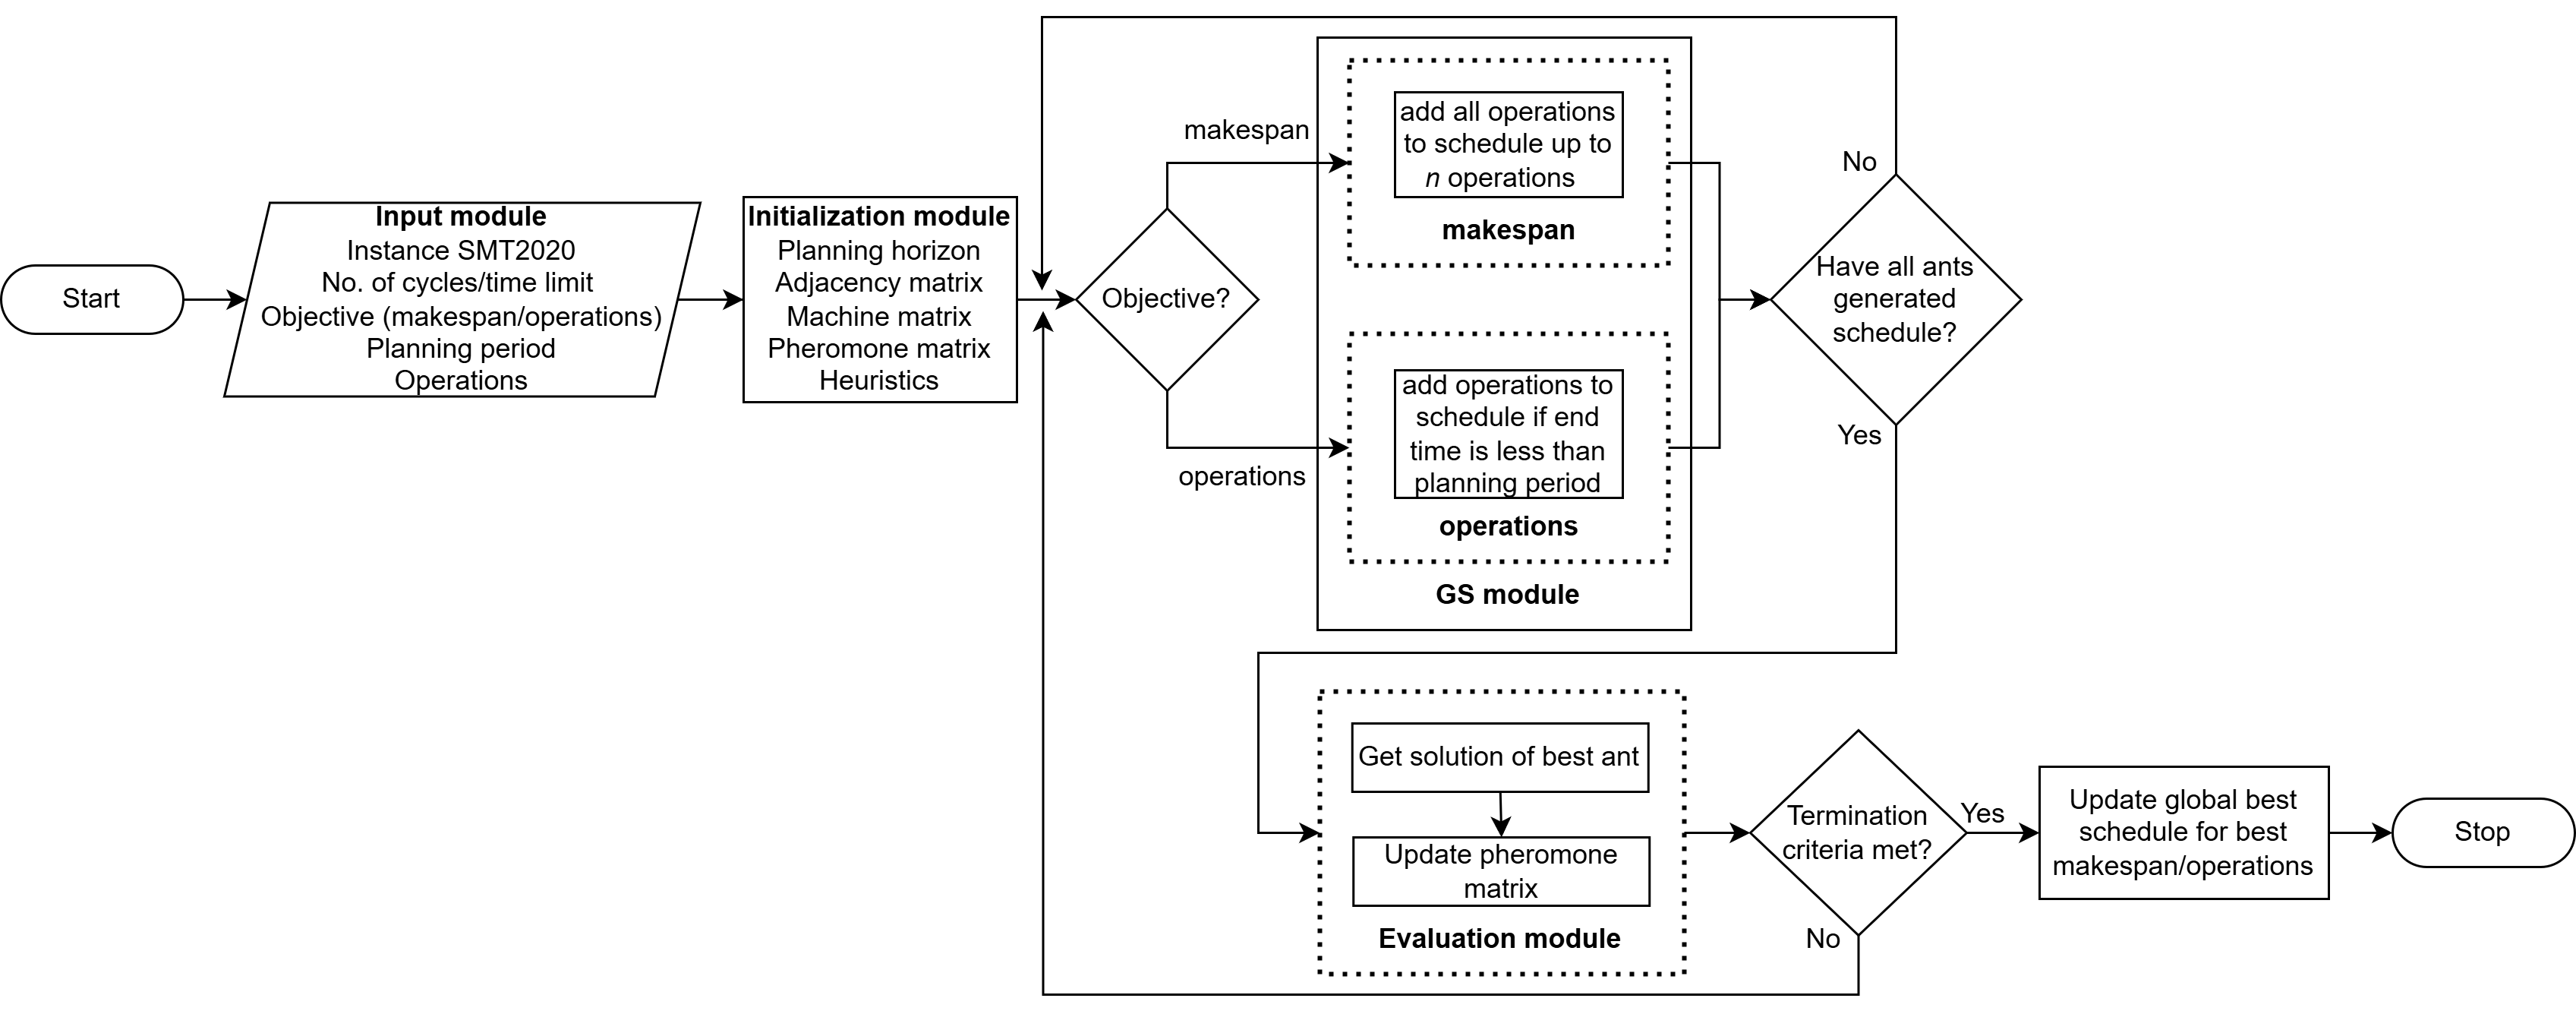
\includegraphics[width=\textwidth]{aco-flowchart.png}
	\caption{GSACO-I framework}
	\label{fig:aco-flowchart}
\end{figure}

Moreover, Algorithm~\ref{gsaco} provides a pseudo-code representation of
GSACO-I for minimizing makespan and optimizing operations.

For a configurable cycle number or time limit~$l$,
each of the $k$ ants applies greedy search
using the GS procedure with respect to the objective.
That is, the first GS phase constructs an operation sequence, which is
then taken as basis for greedily assigning the operations to machines
in the second phase.   
Note that the ants run independently, so that their GS trials
can be performed in parallel.
As a result, $k$ schedules along with edges between operations
(described in Subsection~\ref{subsec:initialization})
that have been selected for their construction are obtained.
If some of these schedules improves the makespan over the best
schedule found in previous iterations (if any),
the best schedule gets updated.
As common for ACO algorithms,
pheromones $\tau_e$ on edges~$e$ are subject to evaporation,
according to the formula $\rho\cdot\tau_e$,
while edges selected to construct the best schedule obtained
so far also receive a pheromone contribution,
calculated as $\tau_e+c$.
Such pheromone deposition increases the chance for edges contributing to the
current best schedule
to get re-selected % by the GS procedure
in forthcoming iterations.

\begin{algorithm}[ht]
	\caption{Greedy Search based ACO (GSACO) for Scheduling}
	\label{gsaco}
	\KwIn{instance, $l$, $o$, $s$, $n$, $h$, $\text{objective}$}
	\KwOut{best schedule found by ants}
	\KwParam{$k$, $\tau_{y}$, $\tau_{z}$, $\rho$, $c$}
	Initialize adjacency, pheromone, and machine matrix\; 
	\eIf{\text{objective} == \text{Makespan}}{
		$\mathit{makespan}\leftarrow \infty$\;
	}{
		$\mathit{operations}\leftarrow 0$\;
	}
	\While{cycle or time limit $l$ is not reached}{
		\ForEach{ant \KwFrom $1$ \KwTo $k$}{
			Run GS procedure to find a schedule\;
		}
		\eIf{\text{objective} == \text{Makespan}}{
			$\mathit{new}\leftarrow$ shortest makespan of ants' schedules\;
			\If{$\mathit{new}<\mathit{makespan}$}{
				$\mathit{makespan}\leftarrow \mathit{new}$\;
				$\mathit{best}\leftarrow$ an ant's schedule of minimum $\mathit{makespan}$\;
			}
		}{
			$\mathit{new}\leftarrow$ maximum operations of ants'\;
			\If{$\mathit{new}>\mathit{operations}$}{
				$\mathit{operations}\leftarrow \mathit{new}$\;
				$\mathit{best}\leftarrow$ an ant's schedule of maximum $\mathit{operations}$\;
			}
		}
		\ForEach{edge $e$ in pheromone matrix}{
			$\tau_{e} \leftarrow \max\{\rho\cdot\tau_e,\tau_z\}$\tcp*[r]{evaporation}
		}
		\ForEach{edge $e$ selected by $\mathit{best}$ ant}{
			$\tau_{e} \leftarrow \tau_e+c$\tcp*[r]{deposit pheromones}
		}
	}
	\Return $\mathit{best}$\;
\end{algorithm}


\subsection{Input Module}
This module reads in an SMSP instance from the SMT2020 simulator develop by \cite{Kovacs2022}, 
and SMT2020 dataset \cite{kopp2020smt2020}.
The instance includes tool groups with their respective machines, jobs currently in progress, and production routes. In terms of dynamic state, the processing times for these routes are stochastic. Conversely, the simulator provides observed averages for processing times and job releases. Additionally, the module takes several inputs for the GSACO optimization process: the objective~$o$, the state of the fab~$s$, planning period~$h$, 
operation per lot~$n$ and a limit~$l$ on either the number of cycles or the time allocated for optimization.


\subsection{Initialization Module}
\label{subsec:initialization}
In view of long production routes with hundreds of operations
in the SMT2020 dataset, we introduce a configurable planning horizon~$n$
as upper bound on the length $n_j$ of the operation sequence for a job~$j$.
The planning horizon thus constitutes a scaling factor for the size and
the resulting complexity of SMSP instances.
% This horizon is crucial in planning and decision-making, especially within large-scale production systems. 
In practice, unpredictable stochastic events make long-term schedules obsolete and necessitate frequent re-scheduling,
where limiting the planning horizon upfront provides a means to
control the search and enable short response times.

To express SMSP as a search problem on graphs,
we identify an instance with the disjunctive graph

whose vertices~$V$ contain the operations $O_{i,j,t}$ plus
a dummy start node~$0$,
conjunctive edges\linebreak[1]%
%
\begin{equation}
	\begin{array}{@{}r@{}l@{}}
		E_c = {}
		& \{(0,O_{1,j,t_1}) \mid O_{1,j,t_1}\in V\}
		\\ {} \cup {}
		& \{(O_{i-1,j,t_{i-1}},O_{i,j,t_i}) \mid O_{i,j,t_i}\in V, i > 1\}
	\end{array}
\end{equation}
%
connect the dummy start node~$0$ to the first operation
and each operation on to its successor (if any) in the sequence for a job,
and disjunctive edges\linebreak[1]%
%
\begin{equation}
	E_d = \{(O_{i,j,t},O_{i',j',t}) \mid O_{i,j,t}\in V,O_{i',j',t}\in V, j\neq j'\}
\end{equation}
%
link operations (of distinct jobs) sharing a common tool group,
as such operations may be allocated to the same machine.

Any feasible schedule induces an acyclic subgraph $(V,E)$ of 
the disjunctive graph~$G$
such that $E_c\subseteq E$, and $(O_{i,j,t},O_{i',j',t})\in E_d\cap E$
iff $s_{i,j,t,m}+d_{i,j,t} < s_{i',j',t,m}$ for distinct jobs $j\neq j'$,
i.e., the operation
$O_{i,j,t}$ is processed before $O_{i',j',t}$ by the same machine~$m$
of tool group $t_m=t$.
Conversely,
the search for a high-quality solution can be accomplished by
determining an acyclic subgraph $(V,E)$ of~$G$ that represents a schedule
of short makespan.

For example, Table~\ref{tab:operations} shows operations
belonging to five jobs, as they can
be obtained with the parameter $n=5$ for the planning period.
Conjunctive edges connect the dummy start node~$0$ to
the operations which come first in their jobs and all operations to their successors.
In addition, mutual disjunctive edges link operations
to be processed on the same tool group.
The resulting $(N+1)\times(N+1)$ adjacency matrix, where $N$ is the
total number of operations, $0$ entries indicate the absence, and
$1$ entries the existence of edges, is given in Figure~\ref{fig:a}.

\begin{table}[ht]
	\caption{Example operations}\label{tab:operations} \centering
	\begin{tabular}{|l|l|l|l|}
		\hline
		No. & Operation & Tool group name & Avg process time (sec)\\ \hline
		$1$ & $O_{1,1,2}$ & TF\_Met\_FE\_45 & $588$ \\
		$2$ & $O_{2,1,3}$ & WE\_FE\_108 & $59$ \\
		$3$ & $O_{3,1,4}$ & WE\_FE\_83 & $62$ \\
		$4$ & $O_{4,1,5}$ & WE\_FE\_84 & $54$ \\
		$5$ & $O_{5,1,1}$ & LithoTrack\_FE\_115 & $130$ \\
		$6$ & $O_{1,2,2}$ & TF\_Met\_FE\_45    & $588$ \\
		$7$ & $O_{2,2,3}$ & WE\_FE\_108 & $59$ \\
		$8$ & $O_{3,2,4}$ & WE\_FE\_83         & $62$ \\
		$9$ & $O_{4,2,5}$ & WE\_FE\_83    & $54$ \\
		$10$ & $O_{5,2,1}$ & LithoTrack\_FE\_115 & $130$ \\
		$11$ & $O_{1,3,2}$ & TF\_Met\_FE\_45         & $588$ \\
		$12$ & $O_{2,3,3}$ & WE\_FE\_108    & $59$ \\
		$13$ & $O_{3,3,4}$ & WE\_FE\_83 & $62$ \\
		$14$ & $O_{4,3,5}$ & WE\_FE\_84         & $54$ \\
		$15$ & $O_{5,3,1}$ & LithoTrack\_FE\_115    & $130$ \\
		$16$ & $O_{1,4,2}$ & TF\_Met\_FE\_45 & $588$ \\
		$17$ & $O_{2,4,3}$ & WE\_FE\_108         & $59$ \\
		$18$ & $O_{3,4,4}$ & WE\_FE\_83    & $62$ \\
		$19$ & $O_{4,4,5}$ & WE\_FE\_84 & $54$ \\
		$20$ & $O_{5,4,1}$ & LithoTrack\_FE\_115         & $130$ \\
		$21$ & $O_{1,5,2}$ & TF\_Met\_FE\_45   & $588$ \\
		$22$ & $O_{2,5,3}$ & WE\_FE\_108 & $59$ \\
		$23$ & $O_{3,5,4}$ & WE\_FE\_83         & $62$ \\
		$24$ & $O_{4,5,5}$ & WE\_FE\_84    & $54$ \\
		$25$ & $O_{5,5,0}$ & LithoTrack\_FE\_115 & $115$ \\
		\hline
	\end{tabular}
\end{table}

\begin{table}[ht]
	\caption{Example instance}\label{tab:instance} \centering
	\begin{tabular}{|l|l|l|}
		\hline
		Lot & Product & Step \\ \hline
		$1$ & $1$ & $1$ \\
		$2$ & $2$ & $2$  \\
		$3$ & $3$ & $1$ \\
		$4$ & $4$ & $3$ \\
		$5$ & $5$ & $1$ \\
		$1$ & $1$ & $2$     \\
		$2$ & $2$ & $1$  \\
		$3$ & $3$ & $3$        \\
		$4$ & $4$ & $1$     \\
		$5$ & $5$ & $2$  \\
		\hline
	\end{tabular}
\end{table}
%

\begin{figure}[h]
	\centering
	\begin{minipage}{.45\columnwidth}
		\centering
		$\begin{array}{c@{}c}
			& \begin{array}{cccccccccc} 0 & 1 & 2 & \dots & 41 & 42 & 43 \end{array} \\
			\begin{array}{c} 0 \\ 1 \\ 2 \\ \vdots \\ 41 \\ 42 \\ 43 \end{array} &
			\left[\begin{array}{ccccccccc}
				0 & 1 & 0 & \dots & 0 & 0 & 1 \\ 
				0 & 0 & 1 & \dots & 0 & 0 & 0 \\ 
				0 & 0 & 0 & \dots & 1 & 0 & 0 \\ 
				\vdots & \vdots & \vdots & \ddots & \vdots & \vdots & \vdots \\
				0 & 0 & 0 & \dots & 0 & 1 & 0 \\ 
				0 & 0 & 0 & \dots & 0 & 0 & 1 \\ 
				0 & 0 & 1 & \dots & 0 & 0 & 0 \\
			\end{array}\right]
		\end{array}$
		\caption{Adjacency matrix for instance in Table~\ref{tab:instance}}
		\label{fig:a}
	\end{minipage}\hfill
	\begin{minipage}{.45\columnwidth}
		\centering
		$\begin{array}{c@{}c}
			& \begin{array}{cccccccccccc} 1 & 2 & 3 & \dots & 10 & 11 & 12 \end{array} \\
			\begin{array}{c} 0 \\ 1 \\ 2 \\ \vdots \\ 41 \\ 42 \\ 43 \end{array} &
			\left[\begin{array}{cccccccccccc}
				0 & 1 & 0 & \dots & 0 & 0 & 0 \\ 
				0 & 0 & 1 & \dots & 0 & 0 & 0 \\ 
				0 & 0 & 0 & \dots & 1 & 0 & 0 \\ 
				\vdots & \vdots & \vdots & \ddots & \vdots & \vdots & \vdots \\
				0 & 0 & 0 & \dots & 0 & 1 & 0 \\ 
				0 & 0 & 0 & \dots & 0 & 0 & 1 \\ 
				0 & 0 & 1 & \dots & 0 & 0 & 0 \\
			\end{array}\right]
		\end{array}$
		\caption{Machine matrix for instance in Table~\ref{tab:instance}}
		\label{fig:b}
	\end{minipage}
\end{figure}

As initial pheromone level on edges $e\in E_c\cup E_d$,
we take $\tau_y=1$ by default.
In general, representing pheromone levels by an $(N+1)\times(N+1)$
matrix similar to the adjacency matrix,
the entries~$\tau_{e}$ are initialized according to the following condition:\linebreak[1]%

\begin{equation}
	\tau_{e} =
	\begin{cases}
		\tau_y & \text{if $e\in E_c\cup E_d$} \\
		0      & \text{otherwise}
	\end{cases}
\end{equation} 

With $\tau_y=1$, this reproduces the adjacency matrix in Figure~\ref{fig:a}
as initial pheromone matrix for our example.

We additionally represent the possible machine assignments
by an $(N+1)\times M$ machine matrix, where $M$ is the total number of
machines.
For example, with two machines per tool group and the mapping
$t_m=\lceil \frac{m}{2} \rceil$ from machine identifiers
$m\in \{1,\dots,12\}$ to the tool groups $t\in\{1,\dots,6\}$,
responsible for processing the remaining operations in Table~\ref{tab:instance},
we obtain the machine matrix shown in Figure~\ref{fig:b}.

\subsection{GS Module}

The general goal of greedy search methods consists of using heuristic decisions
to find high-quality, but not necessarily optimal solutions in short time.
Within GSACO-I, each ant applies greedy search to efficiently construct some
feasible schedule for a given SMSP instance.
The respective GS procedure, outlined by the pseudo-code in Algorithm~\ref{gs-m} and Algorithm~\ref{gs-o},
includes two phases: 
operation sequencing and machine assignment.
%

\begin{algorithm}[t]
	\caption{Greedy Search (GS) Makespan}
	\label{gs-m}
	\KwOut{schedule and selected edges of an an\rlap{t}}
	$\mathit{sequence}\leftarrow[]$\;
	$\mathit{selected}\leftarrow\emptyset$\;
	$\mathit{next}\leftarrow\{(0,O_{1,j,t}) \mid j\in\{1,\dots,J\}\}$\;
	%	\lForEach{$m\in\{1,\dots,M\}$}{$f_m\leftarrow 0$}
	\While{$\mathit{next}\neq\emptyset$}{
		%	$\mathit{\tau}=\sum_{e\in\mathit{next}}\tau_e$\;
		\lForEach{$e\in\mathit{next}$}{%}
		$p_e\leftarrow \frac{\tau_e}{\sum_{e'\in\mathit{next}}\tau_{e'}}$}
	Randomly select an edge $e$ based on $p_e$\;
	\For{selected edge $e=(O',O_{i,j,t})$}{
		$\mathit{sequence}.\mathrm{enqueue}(O_{i,j,t})$\;
		$\mathit{selected}\leftarrow\mathit{selected}\cup\{e\}$\;
		$\mathit{next}\leftarrow\{(O_1,O_2)\in\mathit{next} \mid O_2\neq O_{i,j,t}\}$\;
		$\begin{array}{@{}r@{}l@{}}
			E \leftarrow {} &		
			\{(O_{i,j,t},O_{{i+1},j,t'}) \mid i<n_j\}
			%	  \cup {}
			\\ {} \cup {} &
			\{(O_{i,j,t},O_{i',j',t}) \mid (O_1,O_{i',j',t})\in\mathit{next}\}\text{\;}
		\end{array}$
		$\mathit{next}\leftarrow\mathit{next}\cup E$\;
}}
\lForEach{$m\in\{1,\dots,M\}$}{$a_m\leftarrow 0$}
\While{$\mathit{sequence}\neq[]$}{
	$O_{i,j,t}\leftarrow\mathit{sequence}.\mathrm{dequeue}()$\;
	$a \leftarrow \infty$\;
	%	$b \leftarrow 0$\;
	\ForEach{$m$ \KwFrom $1$ to \KwTo $M$}{
		\If{$t_m = t$ and $a_m < a$}{
			$a\leftarrow a_m$\;
			$b\leftarrow m$\;
		}
	}
	%	\If{$0<b$}{
		$\begin{array}{@{}r@{}l@{}}
			s_{i,j,t,b}\leftarrow 
			\max(&\{a\}
			\\ {} \cup {} &
			\{s_{i-1,j,t',m}+d_{i-1,j,t'}\mid{}i>1\})\text{\;}
		\end{array}
		$
		$a_b \leftarrow s_{i,j,t,b}+d_{i,j,t}$\;
		%	}
}
\Return $\langle\{s_{i,j,t,m} \mid (O',O_{i,j,t})\in\mathit{selected}\},{}$\rlap{$\mathit{selected}\rangle$\;}
\end{algorithm}


\begin{algorithm}[t]
\caption{Greedy Search (GS) Operations}
\label{gs-o}
\KwOut{schedule and selected edges of an an\rlap{t}}
$\mathit{sequence}\leftarrow[]$\;
$\mathit{selected}\leftarrow\emptyset$\;
$\mathit{period}\leftarrow{h}$\;
$\mathit{next}\leftarrow\{(0,O_{1,j,t}) \mid j\in\{1,\dots,J\}\}$\;
%	\lForEach{$m\in\{1,\dots,M\}$}{$f_m\leftarrow 0$}
\While{$\mathit{next}\neq\emptyset$}{
	%	$\mathit{\tau}=\sum_{e\in\mathit{next}}\tau_e$\;
	\lForEach{$e\in\mathit{next}$}{%}
	$p_e\leftarrow \frac{\tau_e}{\sum_{e'\in\mathit{next}}\tau_{e'}}$}
Randomly select an edge $e$ based on $p_e$\;
$\mathit{end time}\leftarrow{e}$\;
\For{selected edge $e=(O',O_{i,j,t})$}{
	$\mathit{e}\leftarrow{start time + process time}$\;
	\If{$\mathit{e}<{period}$}{countinue}
	$\mathit{sequence}.\mathrm{enqueue}(O_{i,j,t})$\;
	$\mathit{selected}\leftarrow\mathit{selected}\cup\{e\}$\;
	$\mathit{next}\leftarrow\{(O_1,O_2)\in\mathit{next} \mid O_2\neq O_{i,j,t}\}$\;
	$\begin{array}{@{}r@{}l@{}}
		E \leftarrow {} &		
		\{(O_{i,j,t},O_{{i+1},j,t'}) \mid i<n_j\}
		%	  \cup {}
		\\ {} \cup {} &
		\{(O_{i,j,t},O_{i',j',t}) \mid (O_1,O_{i',j',t})\in\mathit{next}\}\text{\;}
	\end{array}$
	$\mathit{next}\leftarrow\mathit{next}\cup E$\;
}}
\lForEach{$m\in\{1,\dots,M\}$}{$a_m\leftarrow 0$}
\While{$\mathit{sequence}\neq[]$}{
$O_{i,j,t}\leftarrow\mathit{sequence}.\mathrm{dequeue}()$\;
$a \leftarrow \infty$\;
%	$b \leftarrow 0$\;
\ForEach{$m$ \KwFrom $1$ to \KwTo $M$}{
	\If{$t_m = t$ and $a_m < a$}{
		$a\leftarrow a_m$\;
		$b\leftarrow m$\;
	}
}
%	\If{$0<b$}{
	$\begin{array}{@{}r@{}l@{}}
		s_{i,j,t,b}\leftarrow 
		\max(&\{a\}
		\\ {} \cup {} &
		\{s_{i-1,j,t',m}+d_{i-1,j,t'}\mid{}i>1\})\text{\;}
	\end{array}
	$
	$a_b \leftarrow s_{i,j,t,b}+d_{i,j,t}$\;
	%	}
}
\Return $\langle\{s_{i,j,t,m} \mid (O',O_{i,j,t})\in\mathit{selected}\},{}$\rlap{$\mathit{selected}\rangle$\;}
\end{algorithm}

\subsubsection{GS Makespan}
To minimize makespan, the first phase constructs an ordered list of all operations within an SMSP instance, planned to schedule. This is achieved through a probabilistic decision-making rule derived from the pheromone matrix, which selects edges $(O',O_{i,j,t})$ and sequentially adds their target operations 
$O_{i,j,t}$ to the list. To ensure the feasibility of the resulting schedule, the prerequisite operation 
$O_{i-1,j,t'}$ for the same job~$j$ must already belong to the sequence in case $i>1$. 
This requirement is met by maintaining a set  $\mathit{next}$
of selectable conjunctive and disjunctive edges $(O',O_{i,j,t})$
such that $O'$ is the dummy start node~$0$ or already in sequence,
while $O_{i,j,t}$ is the first yet unsequenced operation of its job~$j$. 

The selection of an edge leading to an unsequenced operation continues until every operation and its corresponding targeting edge has been processed. It is important to note that the chosen disjunctive edges connect operations based on their tool groups, meaning they do not dictate the machine assignments, which are determined in the subsequent phase.

With a complete sequence of operations available, the second phase involves the allocation of each operation to the earliest available machine. This machine assignment step follows the order established in the first phase to create a feasible schedule that assigns machines and start times to all operations.


\subsubsection{GS Operations}
For optimizing operations, the first phase constructs a sequence comprising of all operations
of an SMSP instance that can fit in planning period.
Similarly, a probabilistic decision rule based on the pheromone
matrix selects edges $(O',O_{i,j,t})$
and adds their target operations $O_{i,j,t}$
to the sequence one by one. The operations can only be added to the sequence if the ending time is within the period $h$.
To ensure the feasibility of a resulting schedule,
the predecessor operation $O_{i-1,j,t'}$ of the same job~$j$
must already belong to the sequence in case $i>1$.
This is accomplished by maintaining a set $\mathit{next}$
of selectable conjunctive and disjunctive edges $(O',O_{i,j,t})$
such that $O'$ is the dummy start node~$0$ or already in sequence,
while $O_{i,j,t}$ is the first yet unsequenced operation of its job~$j$.

The process of selecting some edge to a yet unsequenced operation
is repeated until each operation along with an edge targeting it
has been processed.
Note that selected disjunctive edges link operations based on tool groups,
i.e., they do not reflect a machine assignment to be made in the second phase.

With a sequence of operations at hand,
the second phase allocates operations one by one to an earliest
available machine.
The machine assignment process allocates operations
according to the sequence from the first phase, yielding a
feasible schedule that assigns the machines and start times for all operations.

The schedule for minimizing makespan is shown Figure~\ref{fig:sch-makespan}, and a schedule for 15 minutes is shown in Figure~\ref{fig:sch-operations}.

\begin{figure}[t]
	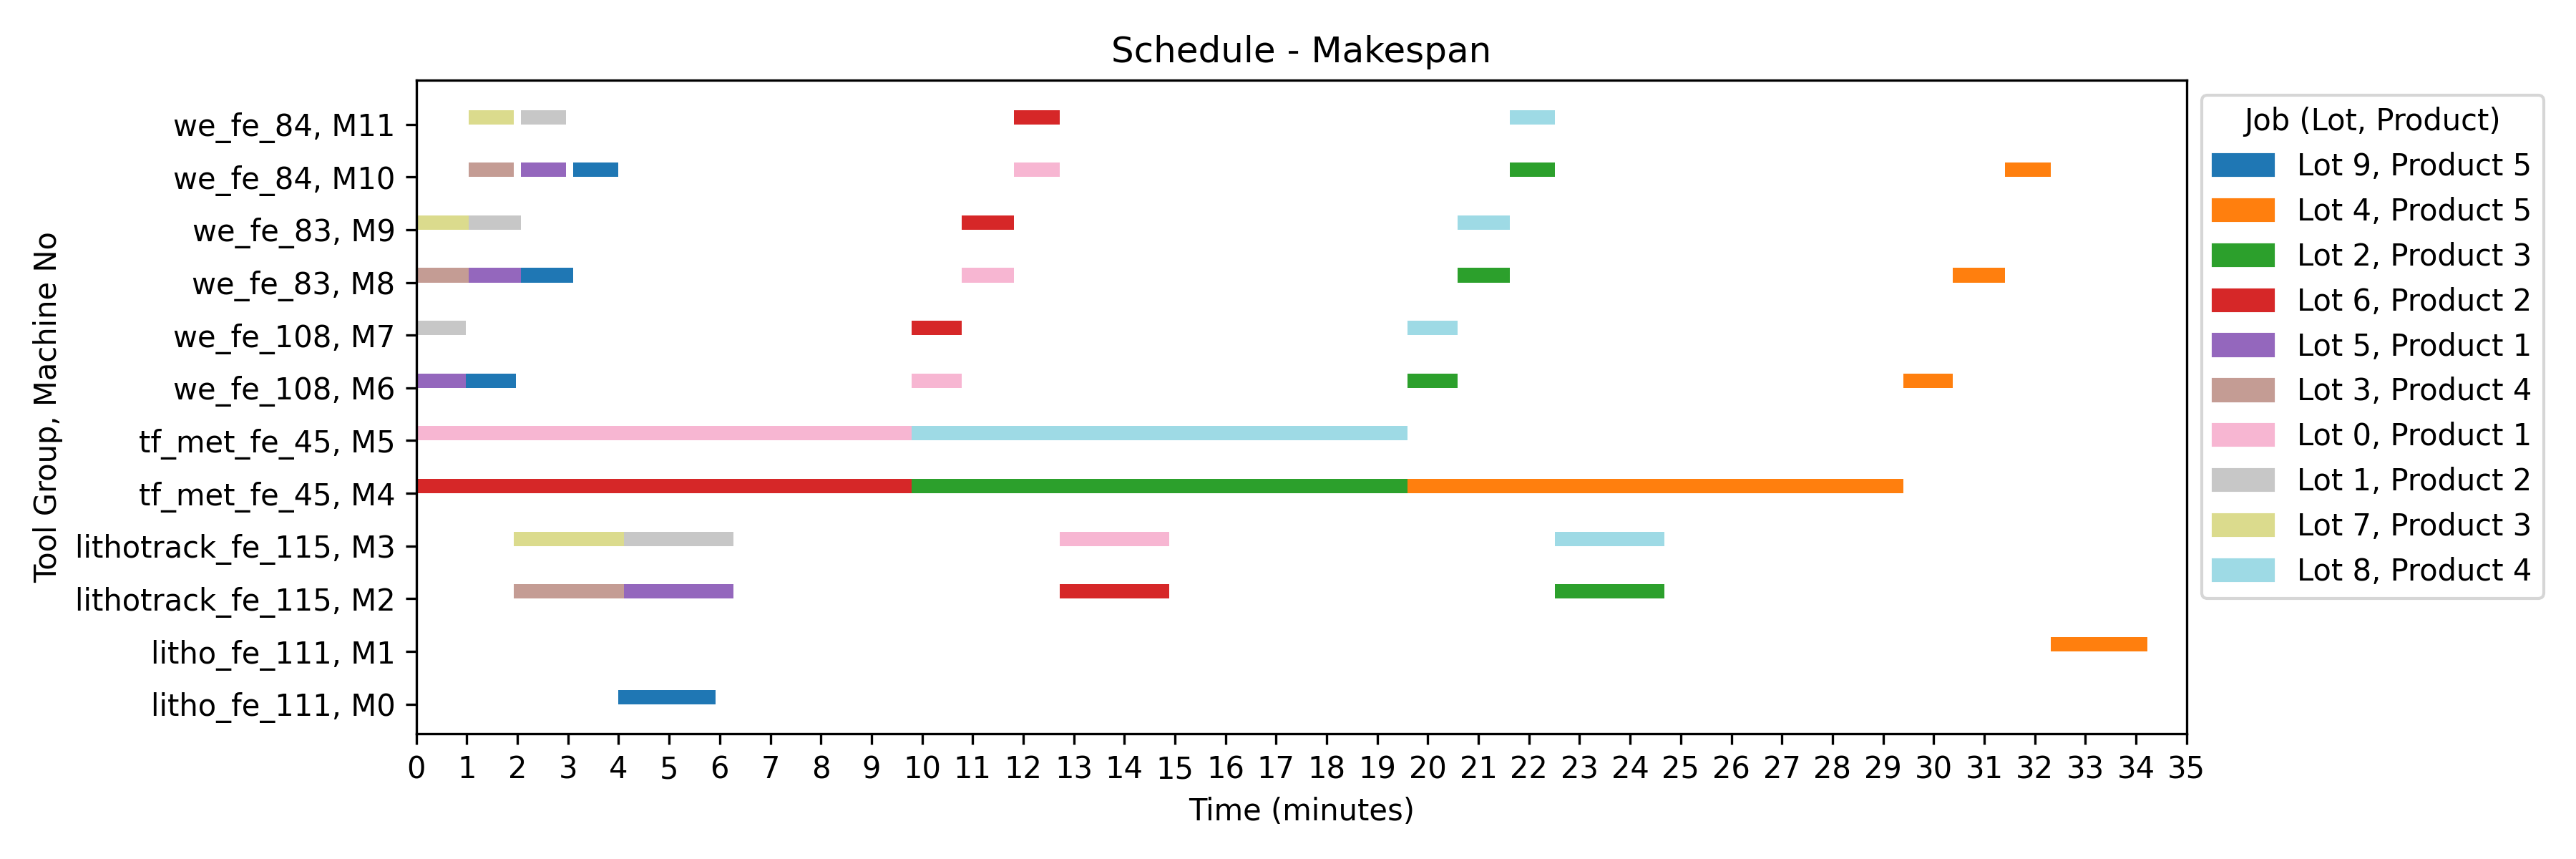
\includegraphics[width=\textwidth]{schedule_example_makespan.png}
	\caption{Feasible schedule for the instance in Table~\ref{tab:instance}}
	\label{fig:sch-makespan}
\end{figure}
\begin{figure}[ht]
	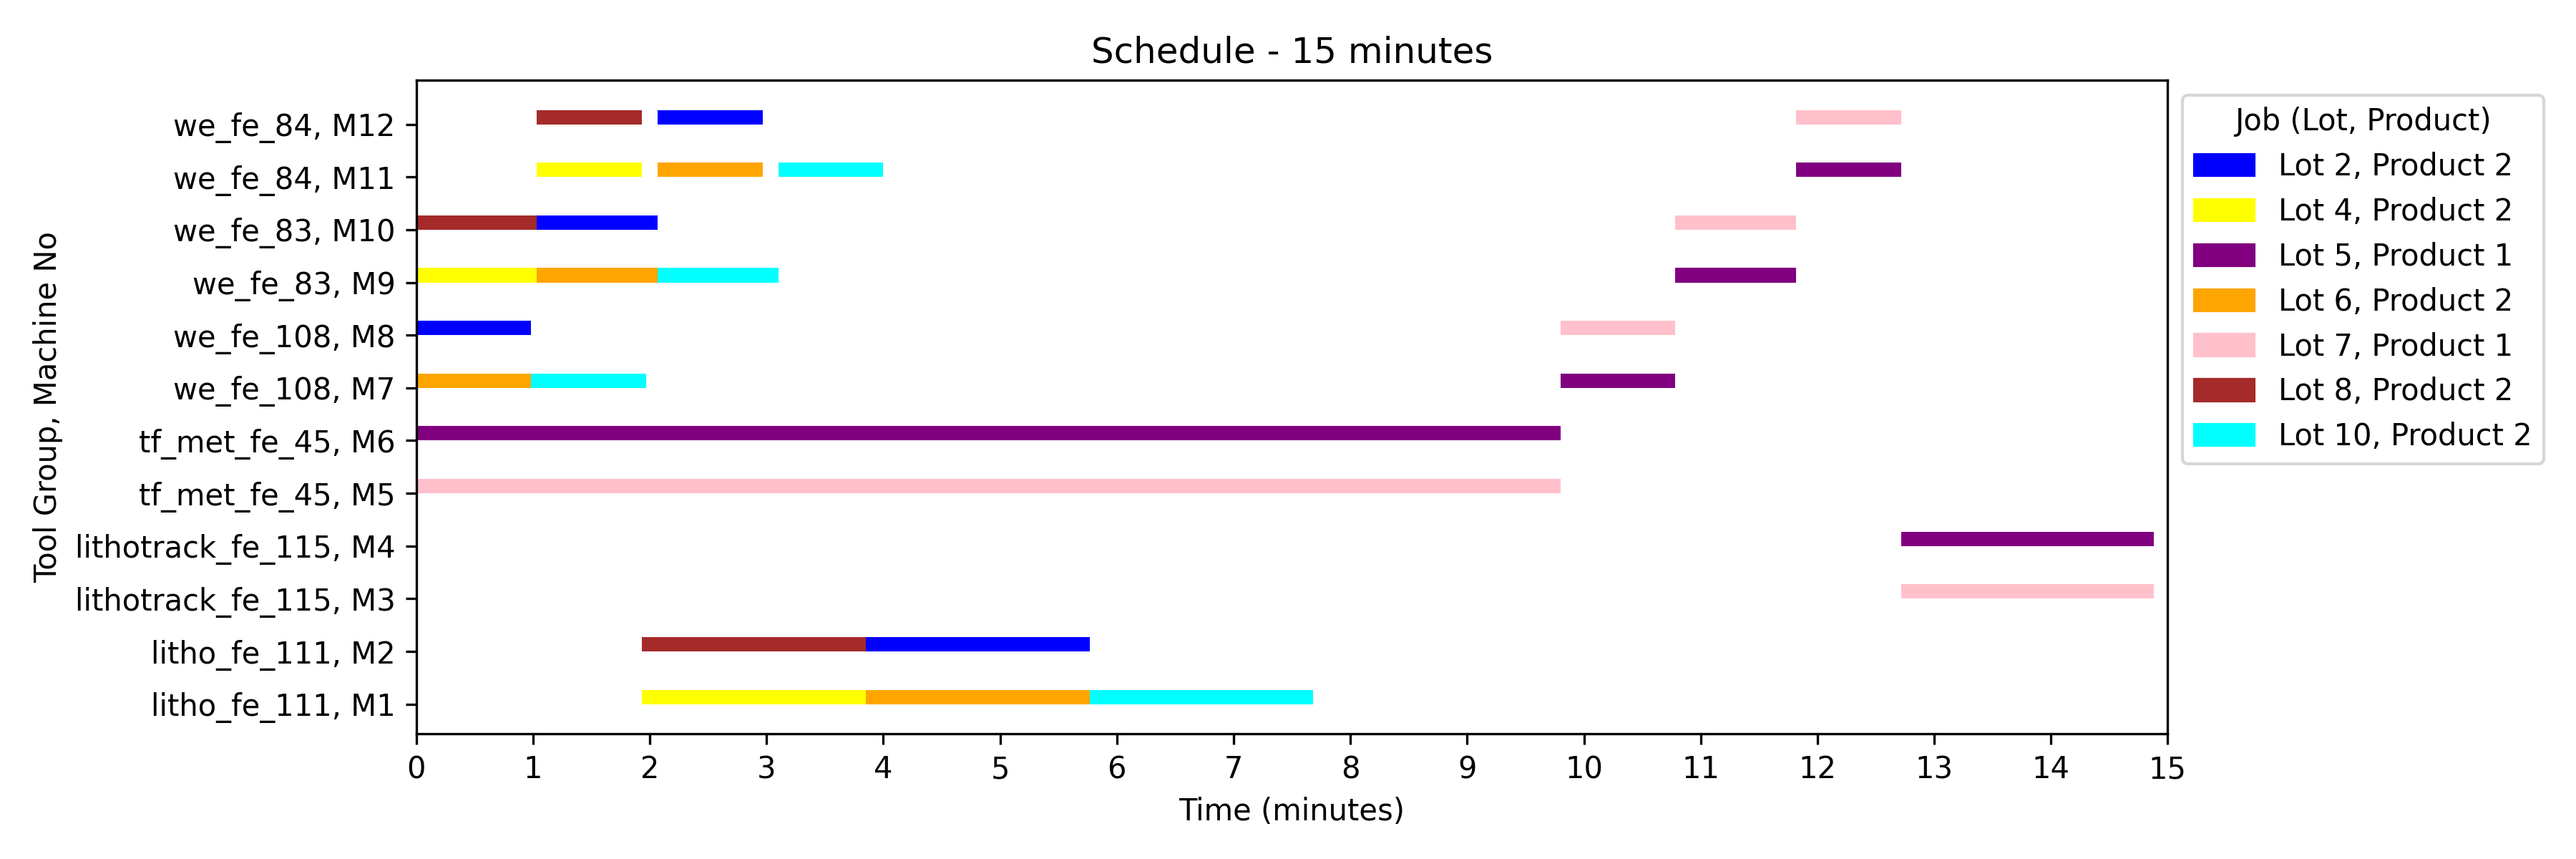
\includegraphics[width=\textwidth]{schedule_example_operations.png}
	\caption{Feasible 15-minutes schedule for the instance in Table~\ref{tab:instance}}
	\label{fig:sch-operations}
\end{figure}


\subsection{Evaluation Module}
While each ant independently constructs a feasible schedule by means of the
GS procedure, the evaluation module collects the results obtained
by the ants in a GSACO iteration.
Among them, a schedule of shortest makespan is determined as outcome of the
iteration and stored as new best solution in case it improves over the schedules found in previous iterations (if any).
After evaporating pheromones~$\tau_e$ by $\rho\cdot\tau_e$,
where $\tau_z$ remains as minimum pheromone level if the obtained value
would be smaller,
the edges~$e$ that have been selected by the GS procedure for constructing the current best schedule receive a pheromone contribution and are updated to $\tau_e+c$.

Note that our contribution parameter $c$ is a constant,
while approaches in the literature often take the inverse of an objective value
\cite{turkyilmaz2020research}, i.e., of the makespan in our case.
The latter requires careful scaling to obtain non-marginal
pheromone contributions, in particular, when makespans get as large
as for SMSP instances.
We instead opt for pheromone contributions such that the
edges selected to construct best schedules are certain to have an increased chance
of getting re-selected in forthcoming iterations.



\section{Simulation}
\label{sec:sim}
To simulate a semiconductor fab, we adapted the simulator developed by \cite{Kovács2022}, enhancing its capacity to handle the complexities and scalability challenges inherent in semiconductor manufacturing scheduling.

This simulator, tailored for the SMT2020 testbed, incorporates a comprehensive framework for the development and validation of innovative scheduling methods without the risk of overfitting. It operates using a dispatcher that dynamically allocates lots to machines based on predefined decision points, facilitating iterative simulation cycles that continue until designated performance benchmarks are achieved.

The dispatcher utilizes basic local rules such as FIFO, CR, and Random selection to manage lot assignments efficiently. These rules serve as foundational strategies, ensuring basic operational efficiency. Additionally, we have integrated enhanced dispatching algorithms derived from the GSACO-I algorithm, which leverage more sophisticated decision-making processes to optimize scheduling tasks further. These enhancements not only improve the precision of the simulation but also significantly extend its applicability and effectiveness in complex manufacturing scenarios.

\begin{figure}[t]
	\includegraphics[width=\textwidth]{sim\_framework.png}
	\caption{Simulator-Scheduler framework}
	\label{fig:ss}
\end{figure}

The framework depicted in Figure~\ref{fig:ss} outlines a sophisticated approach for scheduling operations within a production setting, incorporating both simulation and optimization models to enhance efficiency. At the core, the Input Data Module manages crucial scheduling data, including the SMT2020 dataset that lists lots to be scheduled with their remaining operations, alongside data concerning production objectives and available resources. This information feeds into the initialization processes for both the simulation and optimization modules.

The Simulation Model kicks off with an initialization of instances based on the dataset, where it sets up the environment for running simulations with different dispatching rules—both local and enhanced. Moreover, it generates the average processing time of operations for the scheduling purpose.
The dispatch rules are tested under different processing times to observe their effectiveness in managing operations and lot completions, as well as the flow of work-in-process.

On the optimization side, the GSACO-I algorithm—takes the stage to refine scheduling further. This component iteratively searches for the best or optimal scheduling solutions, assessing each iteration against a criterion to determine if a preferable solution has been achieved. Upon finding the best solution, it finalizes the operations schedule, which details the best sequence and allocation of operations, ready to be implemented to maximize production efficiency.

\section{\uppercase{Experimental Evaluation}}
\label{sec:results}
We implemented GSACO-O algorithm in Python using PyTorch, as it handles tensor operations efficiently and provides a multiprocessing library for
parallelization, thus significantly speeding up the ants' execution of the GS procedure in each GSACO-O iteration.%
\footnote{The source code is publicly available in our GitHub repository:
	\url{https://github.com/prosysscience/GSACO}}
The first challenge consists of determining suitable values for the input
parameters listed in Table~\ref{tab:parameters}, i.e.,
all parameters but the internally calculated pheromone level $\tau_e$ on edges~$e$.
We adhere to the parameters specified in Table~\ref{tab:p_value}, setting a time constraint~$l$ of $10$ minutes for objective makespan and $5$ minutes for objective operations. 
Setting different time limits for these two aspects allows the algorithm to tailor its computational efforts to the specific demands of each task. While makespan optimization seeks the best possible sequence over all operations (requiring extensive computation), optimizing operational efficiency focuses on making quicker adjustments that enhance day-to-day operations without the need for extensive computation. 
For the SMSP instances derived from the SMT2020 dataset, we consider up to $5$ operations per job for minimizing makespan and up to $15$ operations per job for optimizing operational throughput. These parameters are practical, given the stochastic nature of the problem which often necessitates frequent rescheduling. Additionally, we define a short planning horizon~$h$ to accommodate near-term scheduling requirements.
For the initial pheromone level~$\tau_y$,
we start from value~$1$, and take $0.00001$ as the minimum $\tau_z$
to avoid going down to $0$, considering that the GS procedure can only
select edges with non-zero entries in the pheromone matrix.
The values for the number~$k$ of ants, the evaporation rate~$\rho$,
and the pheromone contribution~$c$ are more sophisticated to pick.
That is, we tuned these parameters in a trial-and-error process that,
starting from a baseline, inspects deviations of the final makespan and convergence speed obtained with iterative modifications.
Certainly, an automated approach would be desirable to
perform this task efficiently for new instance sets.%
%
\begin{table}[t]
	\caption{GSACO input parameter values}\label{tab:p_value} \centering
	\begin{tabular}{|l|l|}
		\hline
		Parameter & Value \\ \hline
		$o$ & makespan/operations        \\
		$l$ & $10/5$        \\
		$n$ & $1$--$5$/$15$ \\
		$h$ & $1$--$6$ \\
		$k$ & $10$ \\
		$\tau_{y}$ & $1$ \\
		$\tau_{z}$ & $0.00001$ \\
		%		$\alpha$ & 1  \\
		%		$\beta$ & 1     \\
		$\rho$ & $0.7$ \\
		$c$ & $0.5$ \\
		\hline
	\end{tabular}
\end{table}

To evaluate large-scale SMSP instances,
we consider two semiconductor production scenarios of the SMT2020 dataset:
Low-Volume/High-Mix (LV/HM) and High-Volume/Low-Mix (HV/LM).
As indicated in Table~\ref{tab:Dataset},
both scenarios include more than $2000$ jobs and more than $1300$ machines,
modeling the production processes of modern semiconductor fabs.
The main difference is given by the number of products and associated production routes for jobs, where LV/HM considers $10$ production routes varying between
$200$--$600$ steps in total, while HV/LM comprises $2$ production routes with about
$300$ or $600$ steps, respectively.
Originally, the LV/HM and HV/LM scenarios have been designed to represent fab load at the
start of simulation runs, so that the jobs are at different steps of their
production routes.
We focus on scheduling for operations~$n$ from~$1$ up to~$5$,
to be performed per job.
Hence, the operations $O$ to schedule gradually increase from the
number $J$ of jobs, in case of the operations $n=1$,
% , given in Table~\ref{tab:Dataset},
to more than $10000$ operations % obtained
for the longest % planning 
horizon $n=5$.

\begin{table}[t]
	\caption{Number of jobs, machines, and operations for SMSP instances}\label{tab:Dataset} \centering
	\begin{tabular}{|l|c|c|c|}
		\hline
		Scenario & $J$    & $M$    & $O$              \\ \hline
		LV/HM    & $2156$ & $1313$ & up to $10747$    \\ 
		HV/LM    & $2256$ & $1443$ & up to $11218$    \\
		\hline
	\end{tabular}
\end{table}
%

\begin{table*}[t]
	\caption{SMSP results obtained with CP and GSACO \cite{Ali2024}}\label{tab:results} \centering
	\begin{tabular}{|l|l|l|l|l|l|l|l|l|l|l|l|}
		\hline
		&
		&
		\multicolumn{2}{c|}{$1$ min} &
		\multicolumn{2}{c|}{$3$ min} &
		\multicolumn{2}{c|}{$5$ min} &
		\multicolumn{2}{c|}{$7$ min} &
		\multicolumn{2}{c|}{$9$ min} \\ \cline{3-12} 
		$n$ & Scenario & CP & GSACO & CP & GSACO & CP & GSACO & CP & GSACO & CP & GSACO \\ \hline
		\multirow{2}{*}{$1$} & LV/HM & - & $3735$ & $18572$ & $3725$ & $3746$ & $3725$ & $3723$ & $3725$ & $3723$ & $3725$  \\
		& HV/LM & - & $1405$ & - & $1405$ & $2242$ & $1405$ & $1609$ & $1405$ & $1600$ & $1405$ \\
		\multirow{2}{*}{$2$} & LV/HM & - & $3773$ & - & $3751$ & - & $3750$ & - & $3739$ & $4398$ & $3739$ \\
		& HV/LM & - & $1653$ & - & $1644$ & - & $1611$ & - & $1611$ & - & $1611$   \\
		\multirow{2}{*}{$3$} & LV/HM & - & $3880$ & - & $3867$ & - & $3836$ & - & $3834$ & - & $3834$   \\
		& HV/LM & - & $1902$ & - & $1889$ & - & $1889$ & - & $1876$ & - & $1876$     \\
		\multirow{2}{*}{$4$} & LV/HM & - & $4578$ & - & $4540$ & - & $4540$ & - & $4540$ & - & $4540$     \\
		& HV/LM & - & $2207$ & - & $2113$ & - & $2113$ & - & $2093$ & - & $2093$  \\
		\multirow{2}{*}{$5$} & LV/HM & - & $4680$ & - & $4680$ & - & $4553$ & - & $4553$ & - & $4553$   \\	
		& HV/LM & - & $2667$ & - & $2566$ & - & $2566$ & - & $2518$ & - & $2518$ \\
		\hline  
	\end{tabular}
\end{table*}

While running with a time limit $l$ of $10$ minutes,
Table~\ref{tab:results} reports the makespans of current best schedules
found by the CP solver OR-Tools and our GSACO implementation
at $1$, $3$, $5$, $7$, and $9$ minutes of computing time.
Considering that the SMSP instances are large,
OR-Tools now takes $3$ minutes to come up with the first solution(s)
for the shortest planning horizon $n=1$ on the LV/HM scenario.
Within the same fraction of computing time, GSACO-O already converges to a
makespan of $3725$ and then proceeds with iterations that do not
yield further improvements.
That the best schedule found by GSACO is not optimal is witnessed by a
marginally better solution obtained by OR-Tools after $7$ minutes.
However, for the other SMSP instances, OR-Tools is unable to improve over
GSACO within $9$ minutes, and it cannot even provide feasible schedules
for planning horizons from $n=2$ on the HV/LM scenario or $n=3$ 
on LV/HM.
We performed our experiments on a TUXEDO Pulse 14 Gen1 machine
equipped with an 8-core AMD Ryzen 7 4800H processor at 2.9GHz and onboard
Radeon graphics card.

The quick convergence of our GSACO implementation is also outlined by the makespan improvements plotted in Figure~\ref{fig:makespan}.
On the LV/HM scenario displayed in Figure~\ref{subfig:l}, 
GSACO obtains its best schedules within $7$ minutes
for all planning horizons.
Only for the longest planning horizon $n=5$
on the HV/LM scenario in Figure~\ref{subfig:h},
an improvement occurs after more than the $9$ minutes of computing time
listed in the rightmost column of Table~\ref{tab:results}.
Comparing the SMSP instances for which OR-Tools manages to provide
feasible schedules,
the convergence to makespans in roughly the range of GSACO's results
takes significantly more computing time.
Hence, the time limit that would be necessary to break even with GSACO,
as accomplished within $7$ minutes for the shortest planning horizon
$n=1$ on the LV/HM scenario,
cannot be predicted for the SMSP instances with longer planning horizons.
Moreover, we observe that the initial schedules obtained 
in the first GSACO iteration by some of the ants running in parallel are of relatively high quality, while
OR-Tools sometimes finds outliers as its first solutions.
This phenomenon occurs for the planning horizons $n=1$ and $n=2$
on the LV/HM or HV/LM scenario, respectively, where the latter
schedule of makespan $17664$ is found after more than $9$ minutes
and thus not listed in Table~\ref{tab:results}.%
%
\begin{figure*}[t]
	\centering
	\begin{subfigure}[b]{0.45\linewidth}
		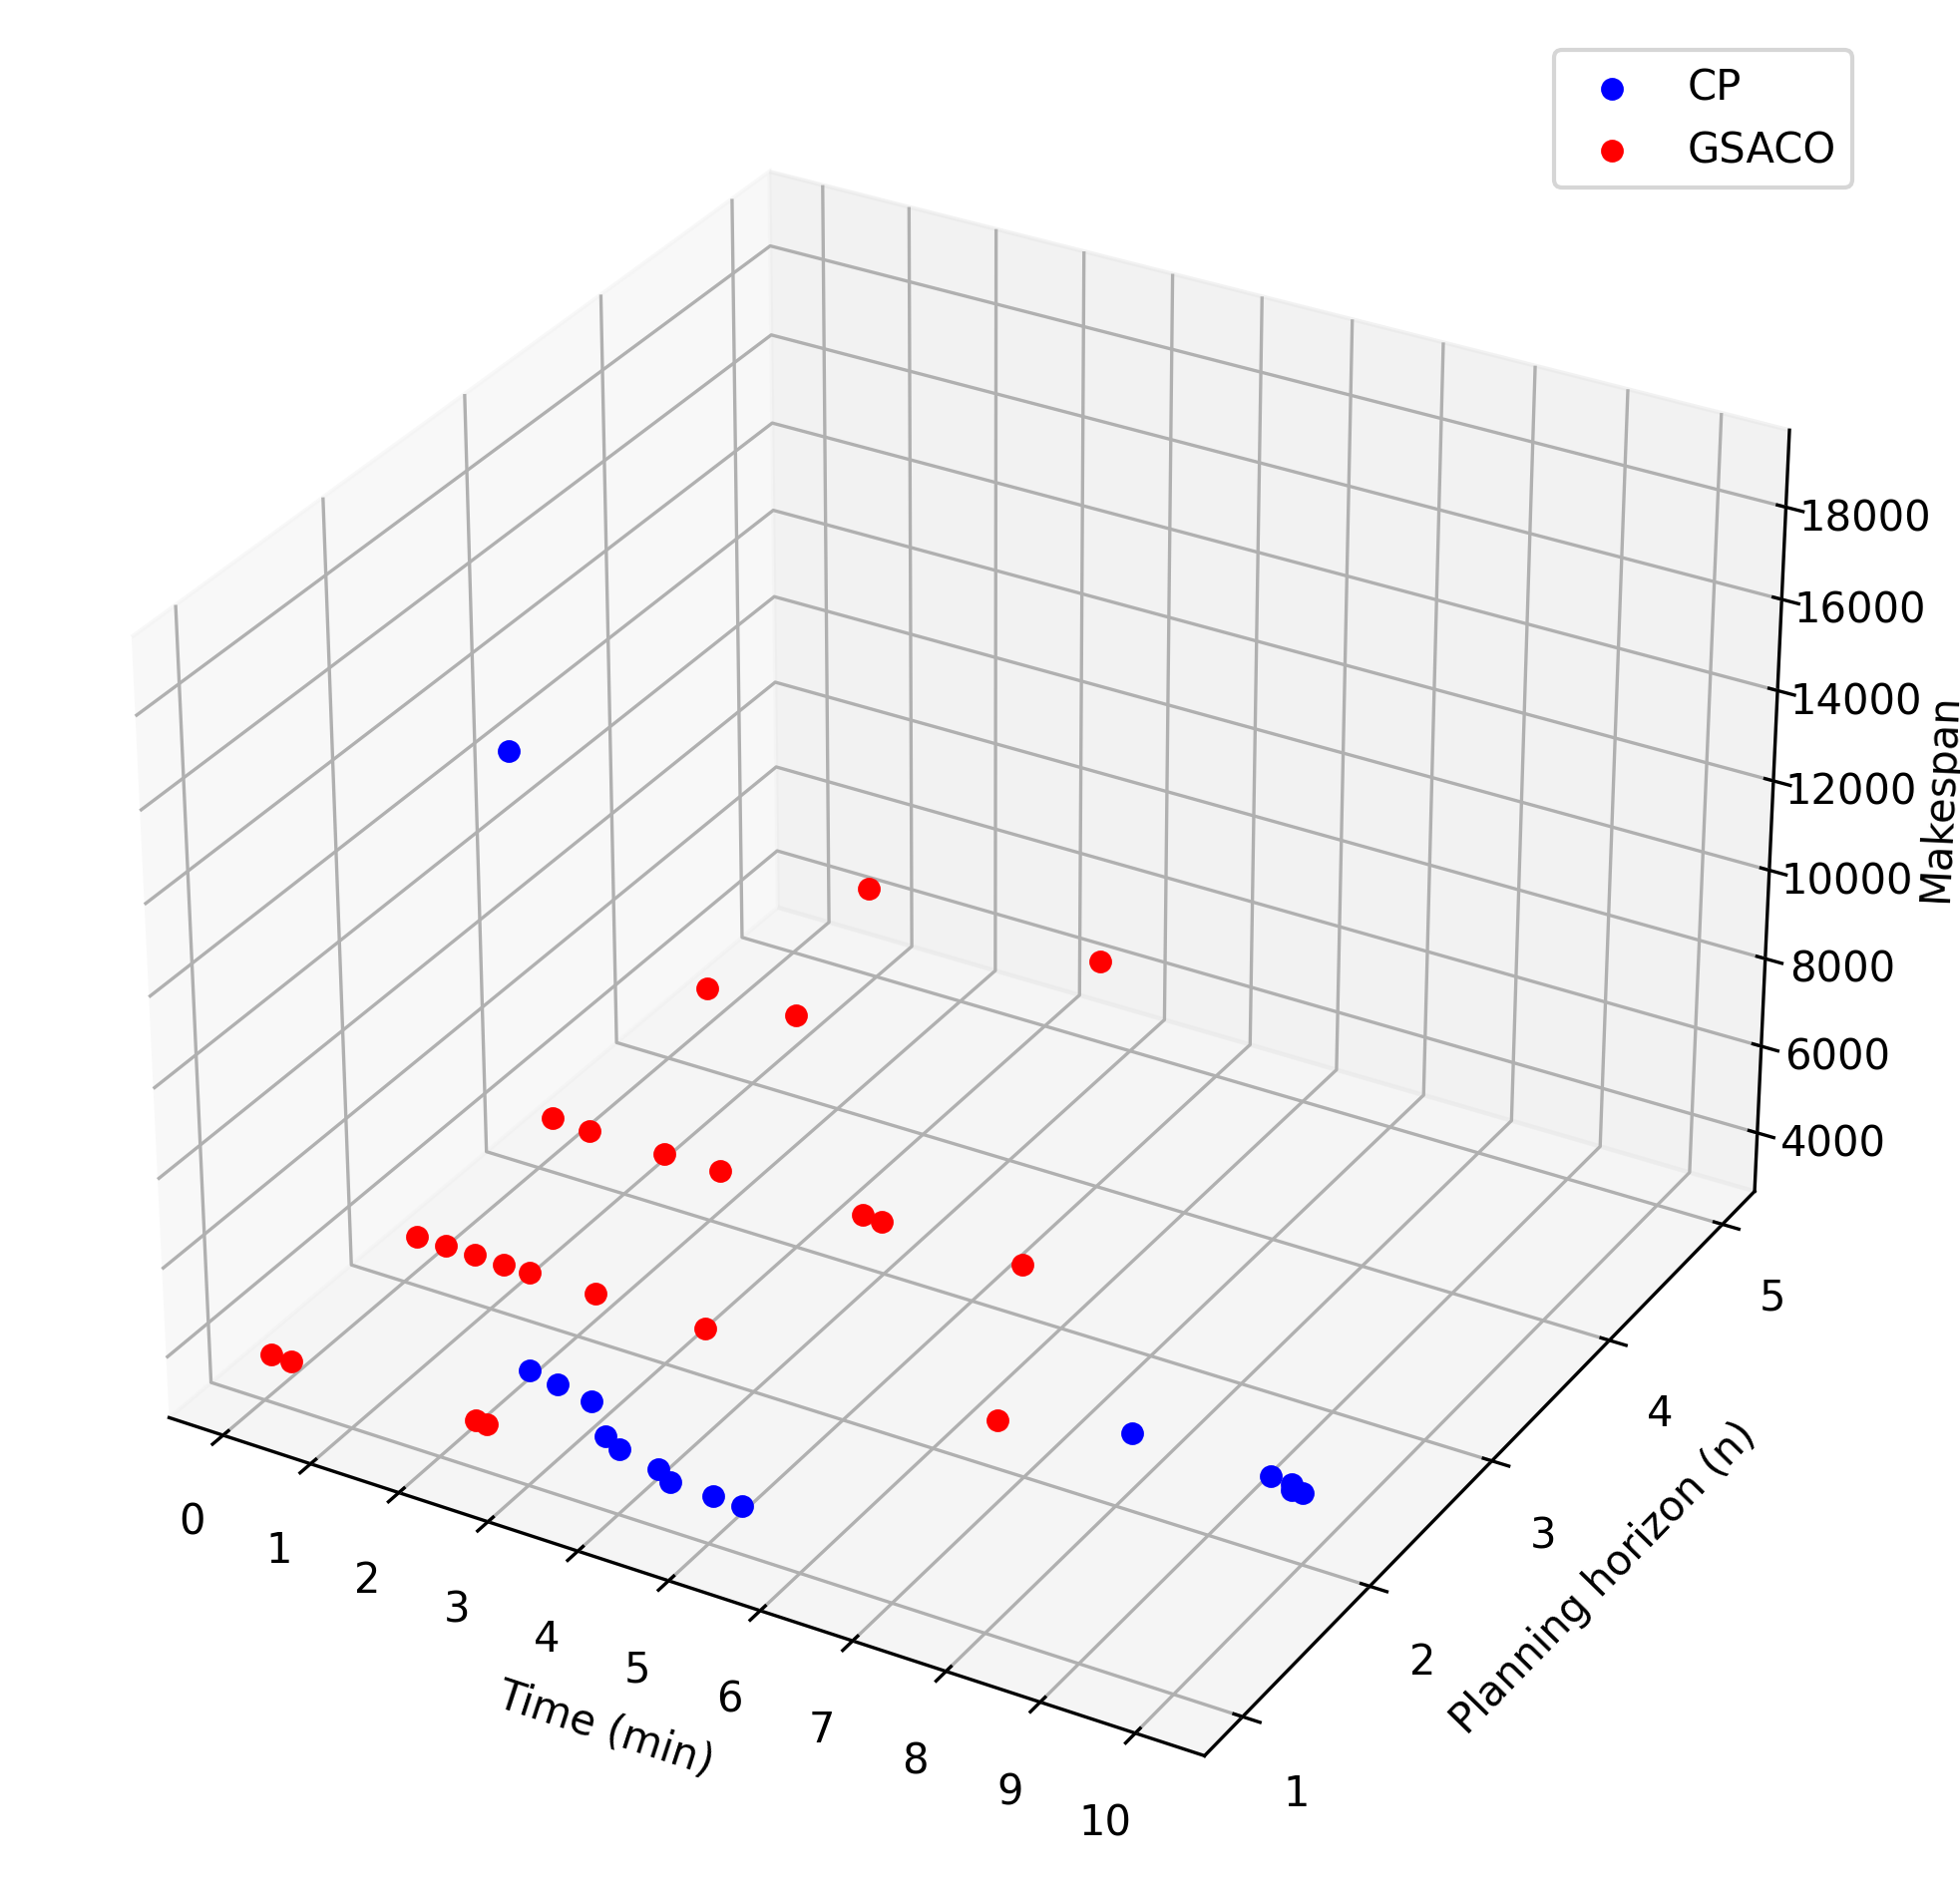
\includegraphics[width=\textwidth]{LVHM.png}
		\caption{LV/HM scenario}
		\label{subfig:l}
	\end{subfigure}
	\hfill
	\begin{subfigure}[b]{0.45\linewidth}
		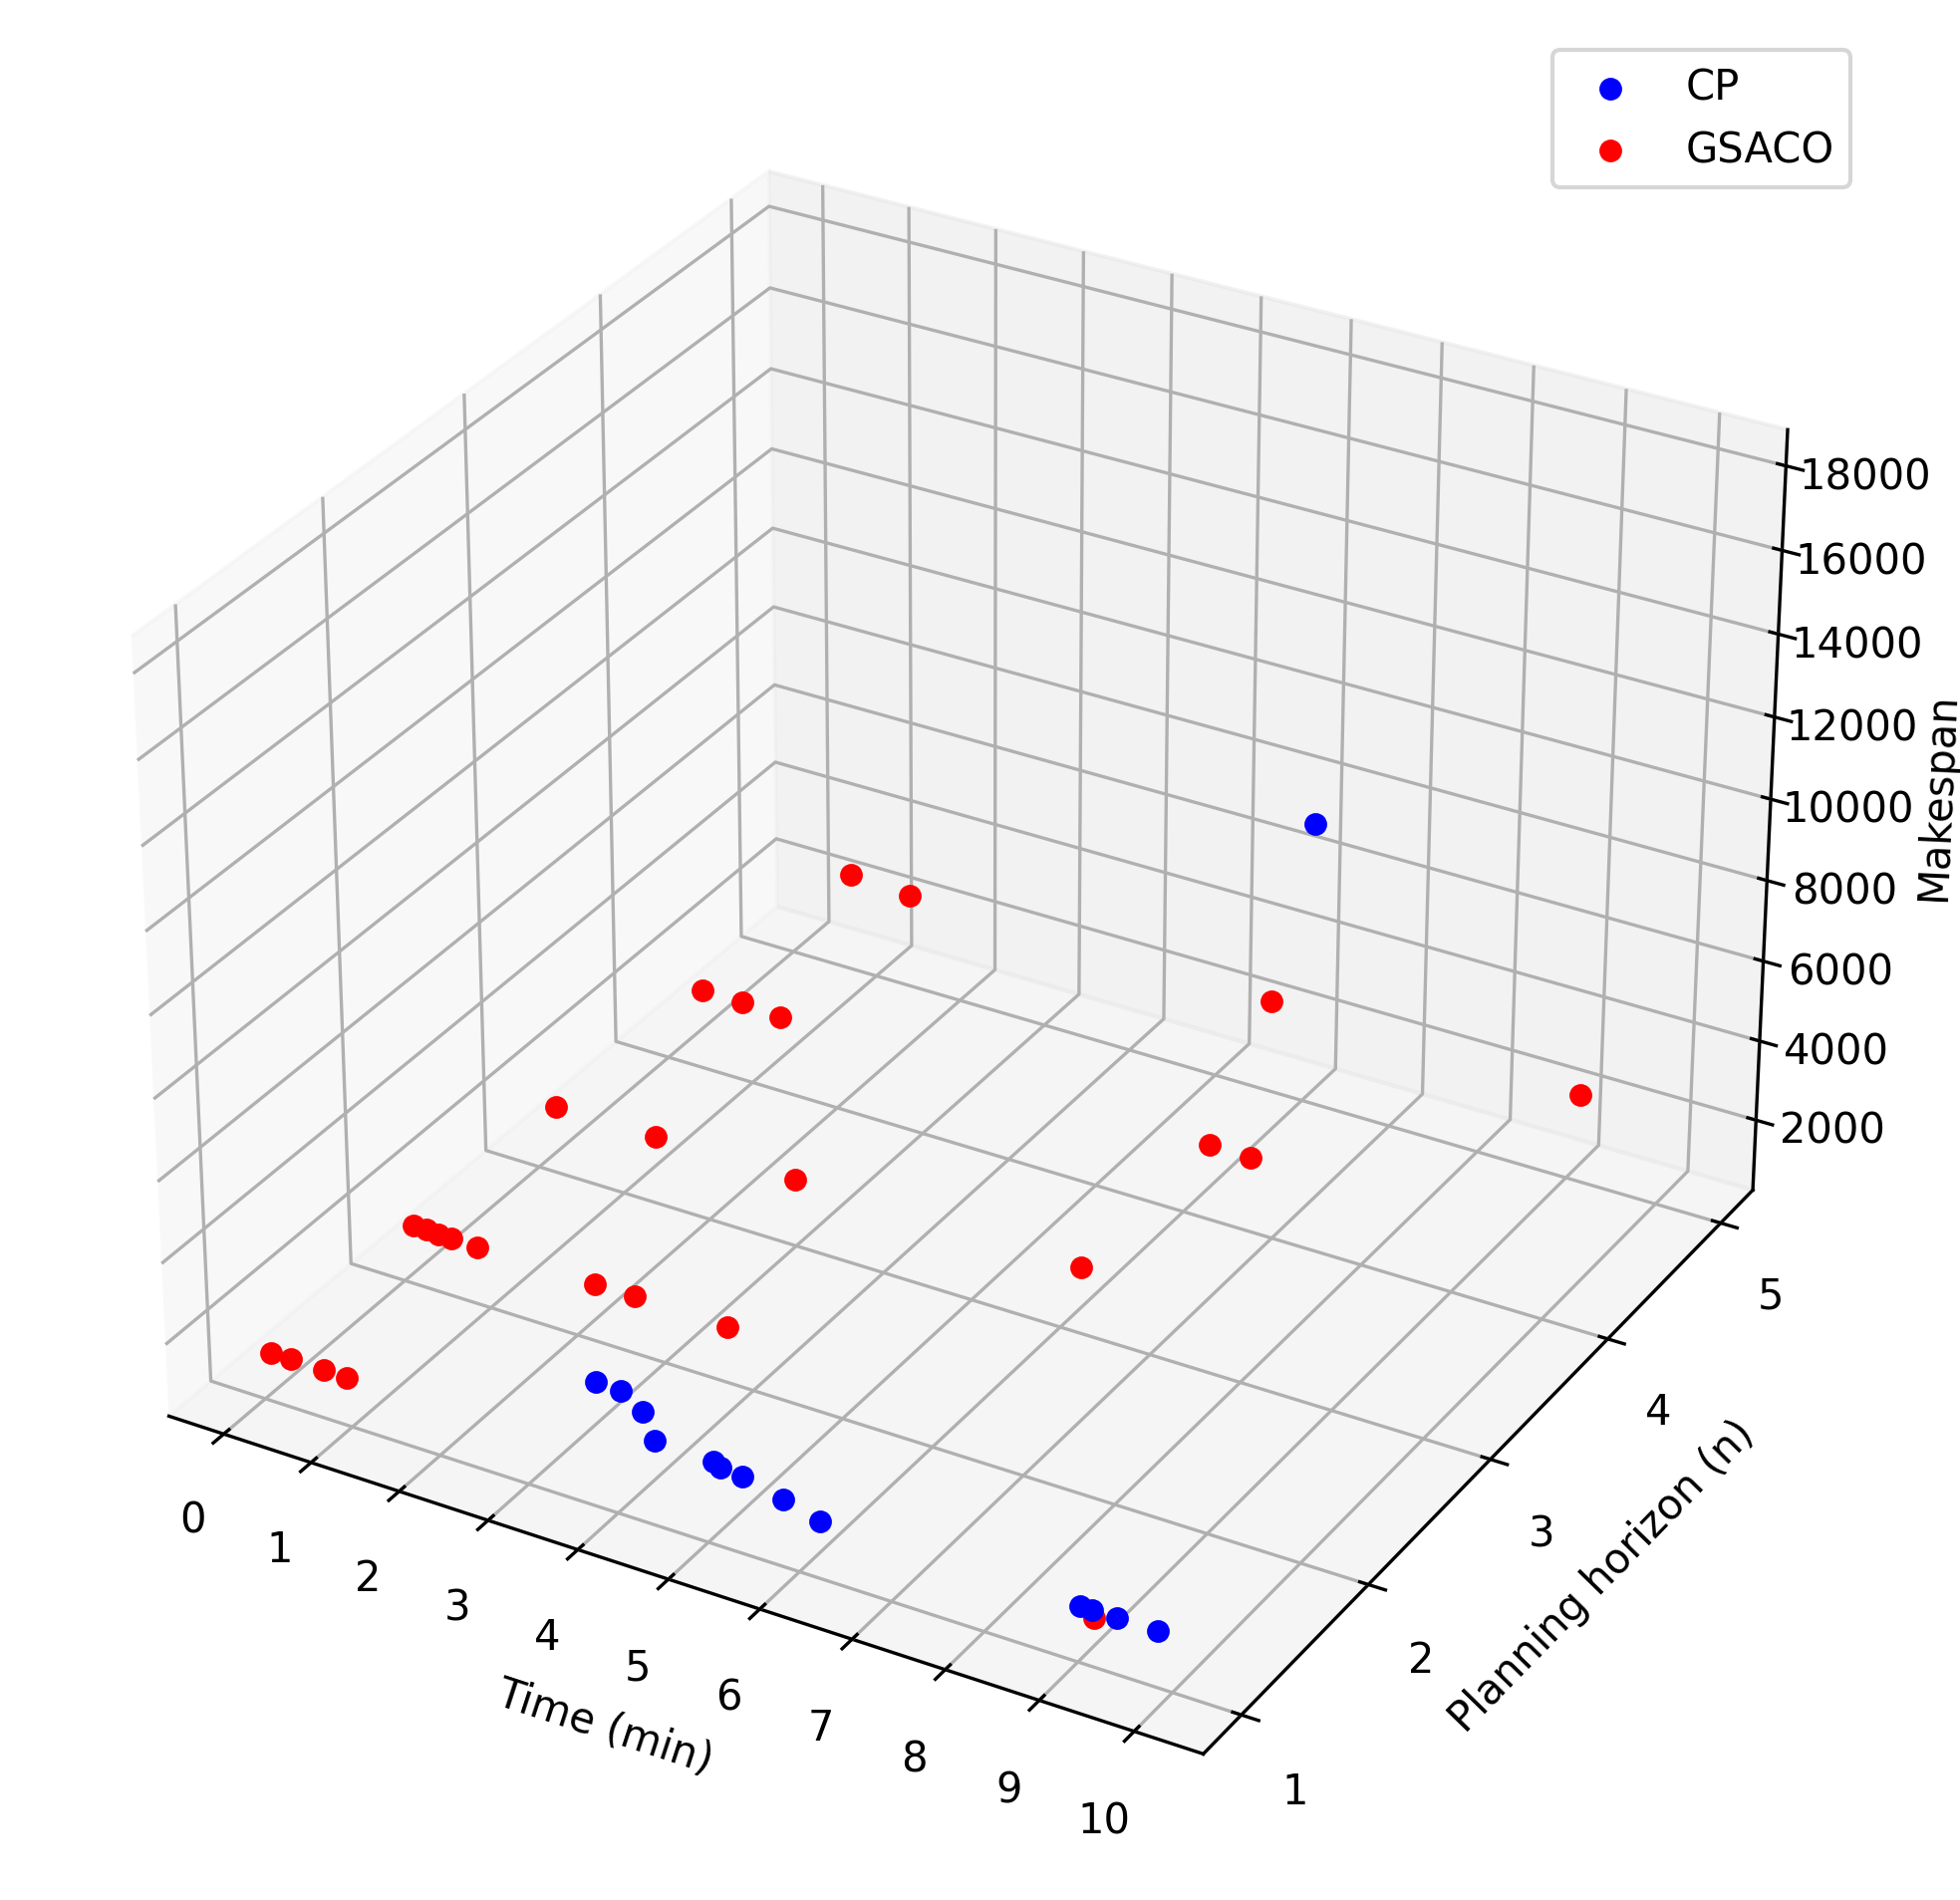
\includegraphics[width=\textwidth]{HVLM.png}
		\caption{HV/LM scenario}
		\label{subfig:h}
	\end{subfigure}
	\caption{Makespan improvements of schedules for SMSP instances obtained with CP and GSACO \cite{Ali2024}\label{fig:makespan}}
\end{figure*}


\begin{table}[t]
	\caption{Comparative performance of dispatching strategies (LV/HM)}
	\label{tab:dispatchers-LVHM}
	\begin{tabular}{|c|lcllllll|ll|}
		\hline
		\multirow{3}{*}{\begin{tabular}[c]{@{}c@{}}Planning \\ horizon\end{tabular}} &
		\multicolumn{8}{c|}{Dispatcher} &
		\multicolumn{2}{c|}{Scheduler} \\ \cline{2-11} 
		&
		\multicolumn{2}{c|}{FIFO} &
		\multicolumn{2}{c|}{CR} &
		\multicolumn{2}{c|}{RANDOM} &
		\multicolumn{2}{c|}{GSACO-O} &
		\multicolumn{2}{c|}{GSACO-O} \\ \cline{2-11} 
		&
		\multicolumn{1}{l|}{Ops/Lots} &
		\multicolumn{1}{l|}{Diff} &
		\multicolumn{1}{l|}{Ops/Lots} &
		\multicolumn{1}{l|}{Diff} &
		\multicolumn{1}{l|}{Ops/Lots} &
		\multicolumn{1}{l|}{Diff} &
		\multicolumn{1}{l|}{Ops/Lots} &
		Diff &
		\multicolumn{1}{l|}{Ops/Lots} &
		diff \\ \hline
		1 &
		\multicolumn{1}{l|}{1419/0} &
		\multicolumn{1}{c|}{-} &
		\multicolumn{1}{l|}{1416/0} &
		\multicolumn{1}{l|}{-0.21\%} &
		\multicolumn{1}{l|}{1403/0} &
		\multicolumn{1}{l|}{-1.12\%} &
		\multicolumn{1}{l|}{1442//0} &
		1.62\% &
		\multicolumn{1}{l|}{1422/0} &
		0.21\% \\
		2 &
		\multicolumn{1}{l|}{2249/0} &
		\multicolumn{1}{c|}{-} &
		\multicolumn{1}{l|}{2328/0} &
		\multicolumn{1}{l|}{3.51\%} &
		\multicolumn{1}{l|}{2275/0} &
		\multicolumn{1}{l|}{1.15\%} &
		\multicolumn{1}{l|}{2409/0} &
		7.11\% &
		\multicolumn{1}{l|}{2368/0} &
		5.29\% \\
		3 &
		\multicolumn{1}{l|}{2384/0} &
		\multicolumn{1}{c|}{-} &
		\multicolumn{1}{l|}{3372/0} &
		\multicolumn{1}{l|}{2.67\%} &
		\multicolumn{1}{l|}{3314/0} &
		\multicolumn{1}{l|}{0.91\%} &
		\multicolumn{1}{l|}{3427/0} &
		4.35\% &
		\multicolumn{1}{l|}{3234/0} &
		-1.52\% \\
		4 &
		\multicolumn{1}{l|}{4018/1} &
		\multicolumn{1}{c|}{-} &
		\multicolumn{1}{l|}{4083/1} &
		\multicolumn{1}{l|}{1.61\%} &
		\multicolumn{1}{l|}{4039/1} &
		\multicolumn{1}{l|}{0.52\%} &
		\multicolumn{1}{l|}{4272/1} &
		6.32\% &
		\multicolumn{1}{l|}{4015/1} &
		-0.07\% \\
		5 &
		\multicolumn{1}{l|}{4901/1} &
		\multicolumn{1}{c|}{-} &
		\multicolumn{1}{l|}{5023/1} &
		\multicolumn{1}{l|}{2.48\%} &
		\multicolumn{1}{l|}{4972/1} &
		\multicolumn{1}{l|}{1.44\%} &
		\multicolumn{1}{l|}{5174/2} &
		5.57\% &
		\multicolumn{1}{l|}{4722/2} &
		-3.65\% \\
		6 &
		\multicolumn{1}{l|}{5665/4} &
		\multicolumn{1}{c|}{-} &
		\multicolumn{1}{l|}{5799/3} &
		\multicolumn{1}{l|}{2.36\%} &
		\multicolumn{1}{l|}{5767/1} &
		\multicolumn{1}{l|}{1.80\%} &
		\multicolumn{1}{l|}{6014/2} &
		6.16\% &
		\multicolumn{1}{l|}{5306/2} &
		-6.33\% \\ \hline
	\end{tabular}%
\end{table}

\begin{table}[t]
	\caption{Comparative performance of dispatching strategies (HV/LM)}
	\label{tab:dispatchers-HVLM}
	\begin{tabular}{|c|lcllllll|ll|}
		\hline
		\multirow{3}{*}{\begin{tabular}[c]{@{}c@{}}Planning \\ horizon\end{tabular}} &
		\multicolumn{8}{c|}{Dispatcher} &
		\multicolumn{2}{c|}{Scheduler} \\ \cline{2-11} 
		&
		\multicolumn{2}{c|}{FIFO} &
		\multicolumn{2}{c|}{CR} &
		\multicolumn{2}{c|}{RANDOM} &
		\multicolumn{2}{c|}{GSACO-O} &
		\multicolumn{2}{c|}{GSACO-O} \\ \cline{2-11} 
		&
		\multicolumn{1}{l|}{Ops/Lots} &
		\multicolumn{1}{l|}{Diff} &
		\multicolumn{1}{l|}{Ops/Lots} &
		\multicolumn{1}{l|}{Diff} &
		\multicolumn{1}{l|}{Ops/Lots} &
		\multicolumn{1}{l|}{Diff} &
		\multicolumn{1}{l|}{Ops/Lots} &
		Diff &
		\multicolumn{1}{l|}{Ops/Lots} &
		Diff \\ \hline
		1 &
		\multicolumn{1}{l|}{1821/0} &
		\multicolumn{1}{c|}{-} &
		\multicolumn{1}{l|}{1798/0} &
		\multicolumn{1}{l|}{-1.26\%} &
		\multicolumn{1}{l|}{1810/0} &
		\multicolumn{1}{l|}{-0.60\%} &
		\multicolumn{1}{l|}{1831/0} &
		0.54\% &
		\multicolumn{1}{l|}{1848/0} &
		1.48\% \\
		2 &
		\multicolumn{1}{l|}{2831/0} &
		\multicolumn{1}{c|}{-} &
		\multicolumn{1}{l|}{2811/0} &
		\multicolumn{1}{l|}{-0.71\%} &
		\multicolumn{1}{l|}{2852/0} &
		\multicolumn{1}{l|}{0.74\%} &
		\multicolumn{1}{l|}{2957/0} &
		4.45\% &
		\multicolumn{1}{l|}{2960/0} &
		4.55\% \\
		3 &
		\multicolumn{1}{l|}{4020/1} &
		\multicolumn{1}{c|}{-} &
		\multicolumn{1}{l|}{4021/1} &
		\multicolumn{1}{l|}{0.02\%} &
		\multicolumn{1}{l|}{4065/1} &
		\multicolumn{1}{l|}{1.12\%} &
		\multicolumn{1}{l|}{4162/1} &
		3.53\% &
		\multicolumn{1}{l|}{4093/1} &
		1.81\% \\
		4 &
		\multicolumn{1}{l|}{4914/4} &
		\multicolumn{1}{c|}{-} &
		\multicolumn{1}{l|}{4934/3} &
		\multicolumn{1}{l|}{0.40\%} &
		\multicolumn{1}{l|}{4975/3} &
		\multicolumn{1}{l|}{1.24\%} &
		\multicolumn{1}{l|}{5118/3} &
		4.15\% &
		\multicolumn{1}{l|}{4970/3} &
		1.07\% \\
		5 &
		\multicolumn{1}{l|}{5960/6} &
		\multicolumn{1}{c|}{-} &
		\multicolumn{1}{l|}{6003/5} &
		\multicolumn{1}{l|}{0.72\%} &
		\multicolumn{1}{l|}{6026/5} &
		\multicolumn{1}{l|}{1.10\%} &
		\multicolumn{1}{l|}{6263/5} &
		5.08\% &
		\multicolumn{1}{l|}{5975/5} &
		0.25\% \\
		6 &
		\multicolumn{1}{l|}{6841/8} &
		\multicolumn{1}{c|}{-} &
		\multicolumn{1}{l|}{6946/8} &
		\multicolumn{1}{l|}{1.53\%} &
		\multicolumn{1}{l|}{6973/9} &
		\multicolumn{1}{l|}{1.92\%} &
		\multicolumn{1}{l|}{7162/7} &
		4.69\% &
		\multicolumn{1}{l|}{6716/7} &
		-1.82\% \\ \hline
	\end{tabular}%
\end{table}

Furthermore, this study investigates the efficiency of various dispatching strategies in a simulated manufacturing environment. Dispatchers play a critical role in production systems by determining the order in which jobs are processed. Effective dispatching can significantly enhance operational throughput and resource utilization. To this end, we compare traditional and enhanced dispatching based on a GSACO-O. The primary objective is to quantify and compare the performance changes of different dispatching strategies over multiple planning horizons.

We examine the efficacy of four distinct dispatching strategies using two different datasets, characterized as High Volume Low Mix (HV/LM) and Low Volume High Mix (LV/HM), to evaluate their effectiveness across six varied planning horizons. The dispatching strategies include FIFO, CR, RANDOM, and GSACO-O, which is also assessed as a scheduler. The performance metrics were recorded in terms of operations and lots completed, with FIFO serving as the baseline for performance comparison.

The results from the LV/HM dataset shown in Table~\ref{tab:dispatchers-LVHM} indicate variable performance across the strategies and horizons. FIFO maintained consistent throughput but was generally outperformed by our GSACO-O dispatcher, which showed substantial increases in operational efficiency. Similarly, the results from HV/LM dataset shown in Table~\ref{tab:dispatchers-HVLM} further substantiate the superior performance of the GSACO-O strategy, confirming its effectiveness across different planning horizons.

The poor performance of GSACO-O over long planning horizon, as a scheduler compared to its role as a dispatcher can be attributed to the operational complexities. While dispatching focuses on immediate, localized decision-making related to the sequence and priority of jobs within the manufacturing process, scheduling involves long-term planning, requiring the management of more complex variables over extended periods. The GSACO-O algorithm, which combines greedy search and swarm intelligence, excels in environments where data is abundant and immediate adaptability is crucial, making it highly effective for dispatching. However, as a scheduler, the algorithm must contend with uncertainties such as fluctuating future orders and resource availability, which may not be as predictable as the current operational statuses utilized in dispatching. Moreover, the effectiveness of a scheduler is often gauged on long-term outcomes such as overall resource utilization and job load balancing, metrics that require a different approach or algorithmic tuning than those used for dispatching tasks.

\begin{figure}[t]
	\centering
	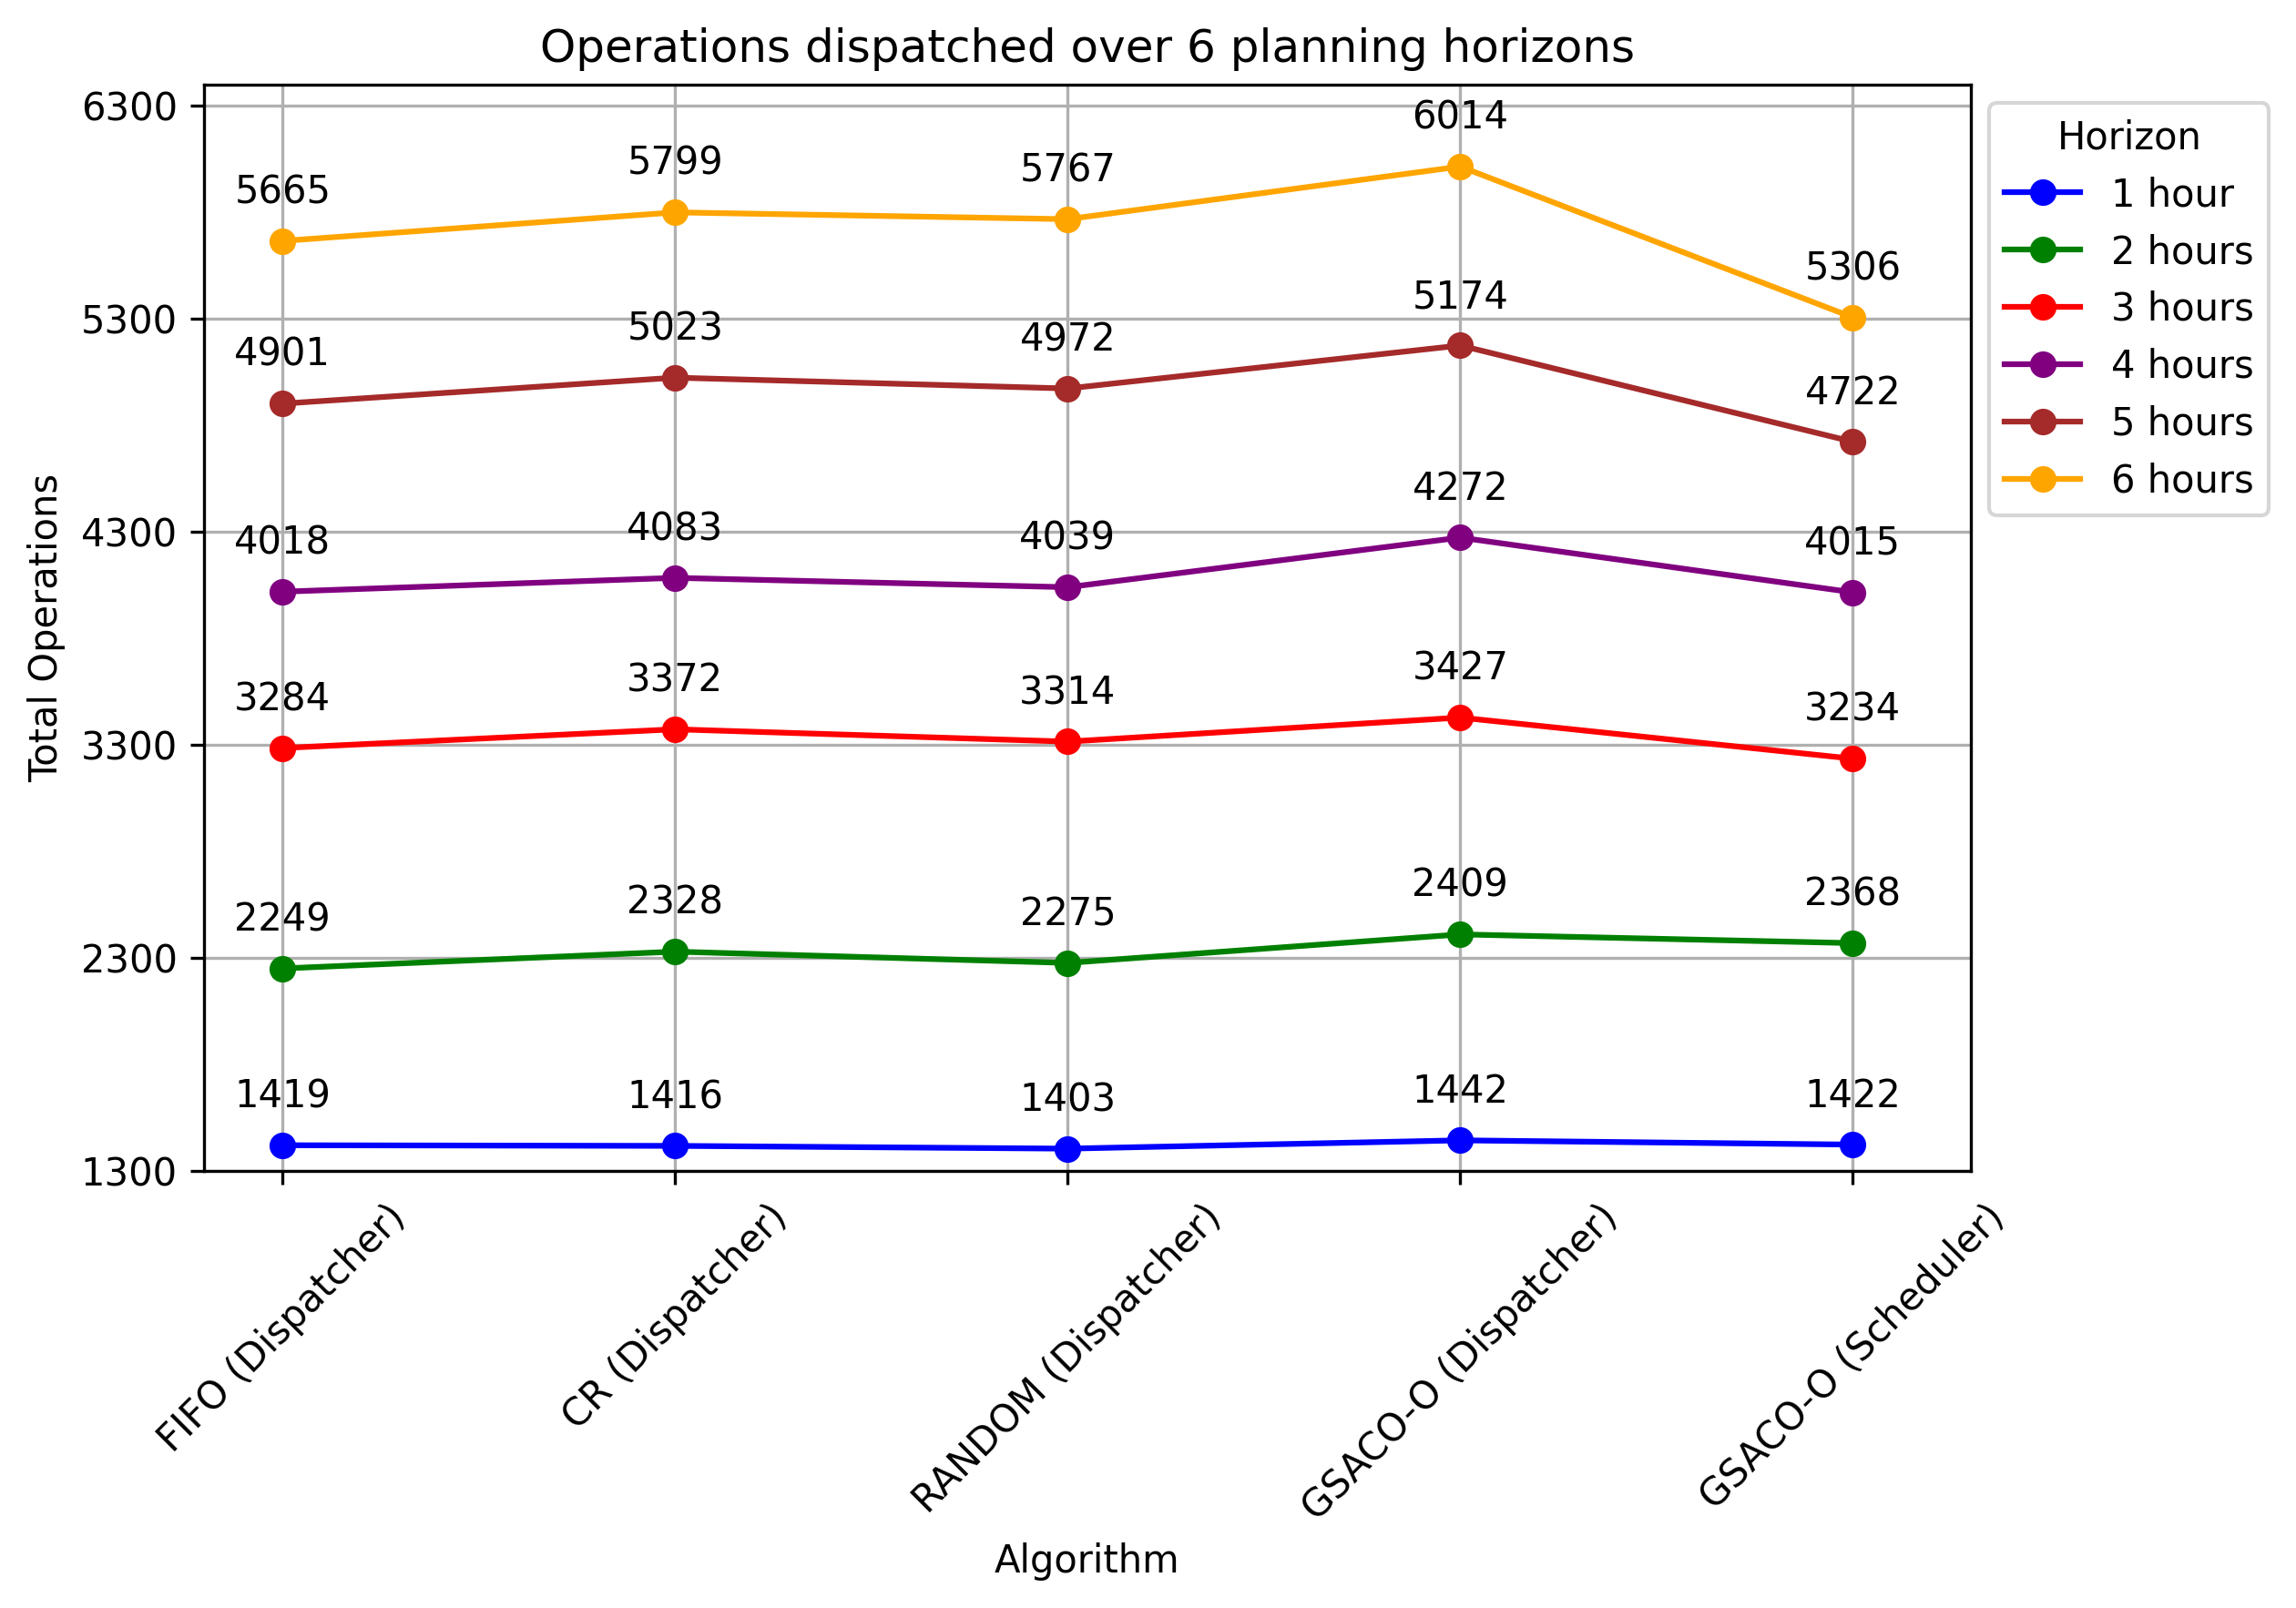
\includegraphics[width=\textwidth]{LVHM/operations_LVHM.png}
	\caption{Operations throughput (LV/HM)}
	\label{fig:totalopsLVHM}
\end{figure}

\begin{figure}[t]
	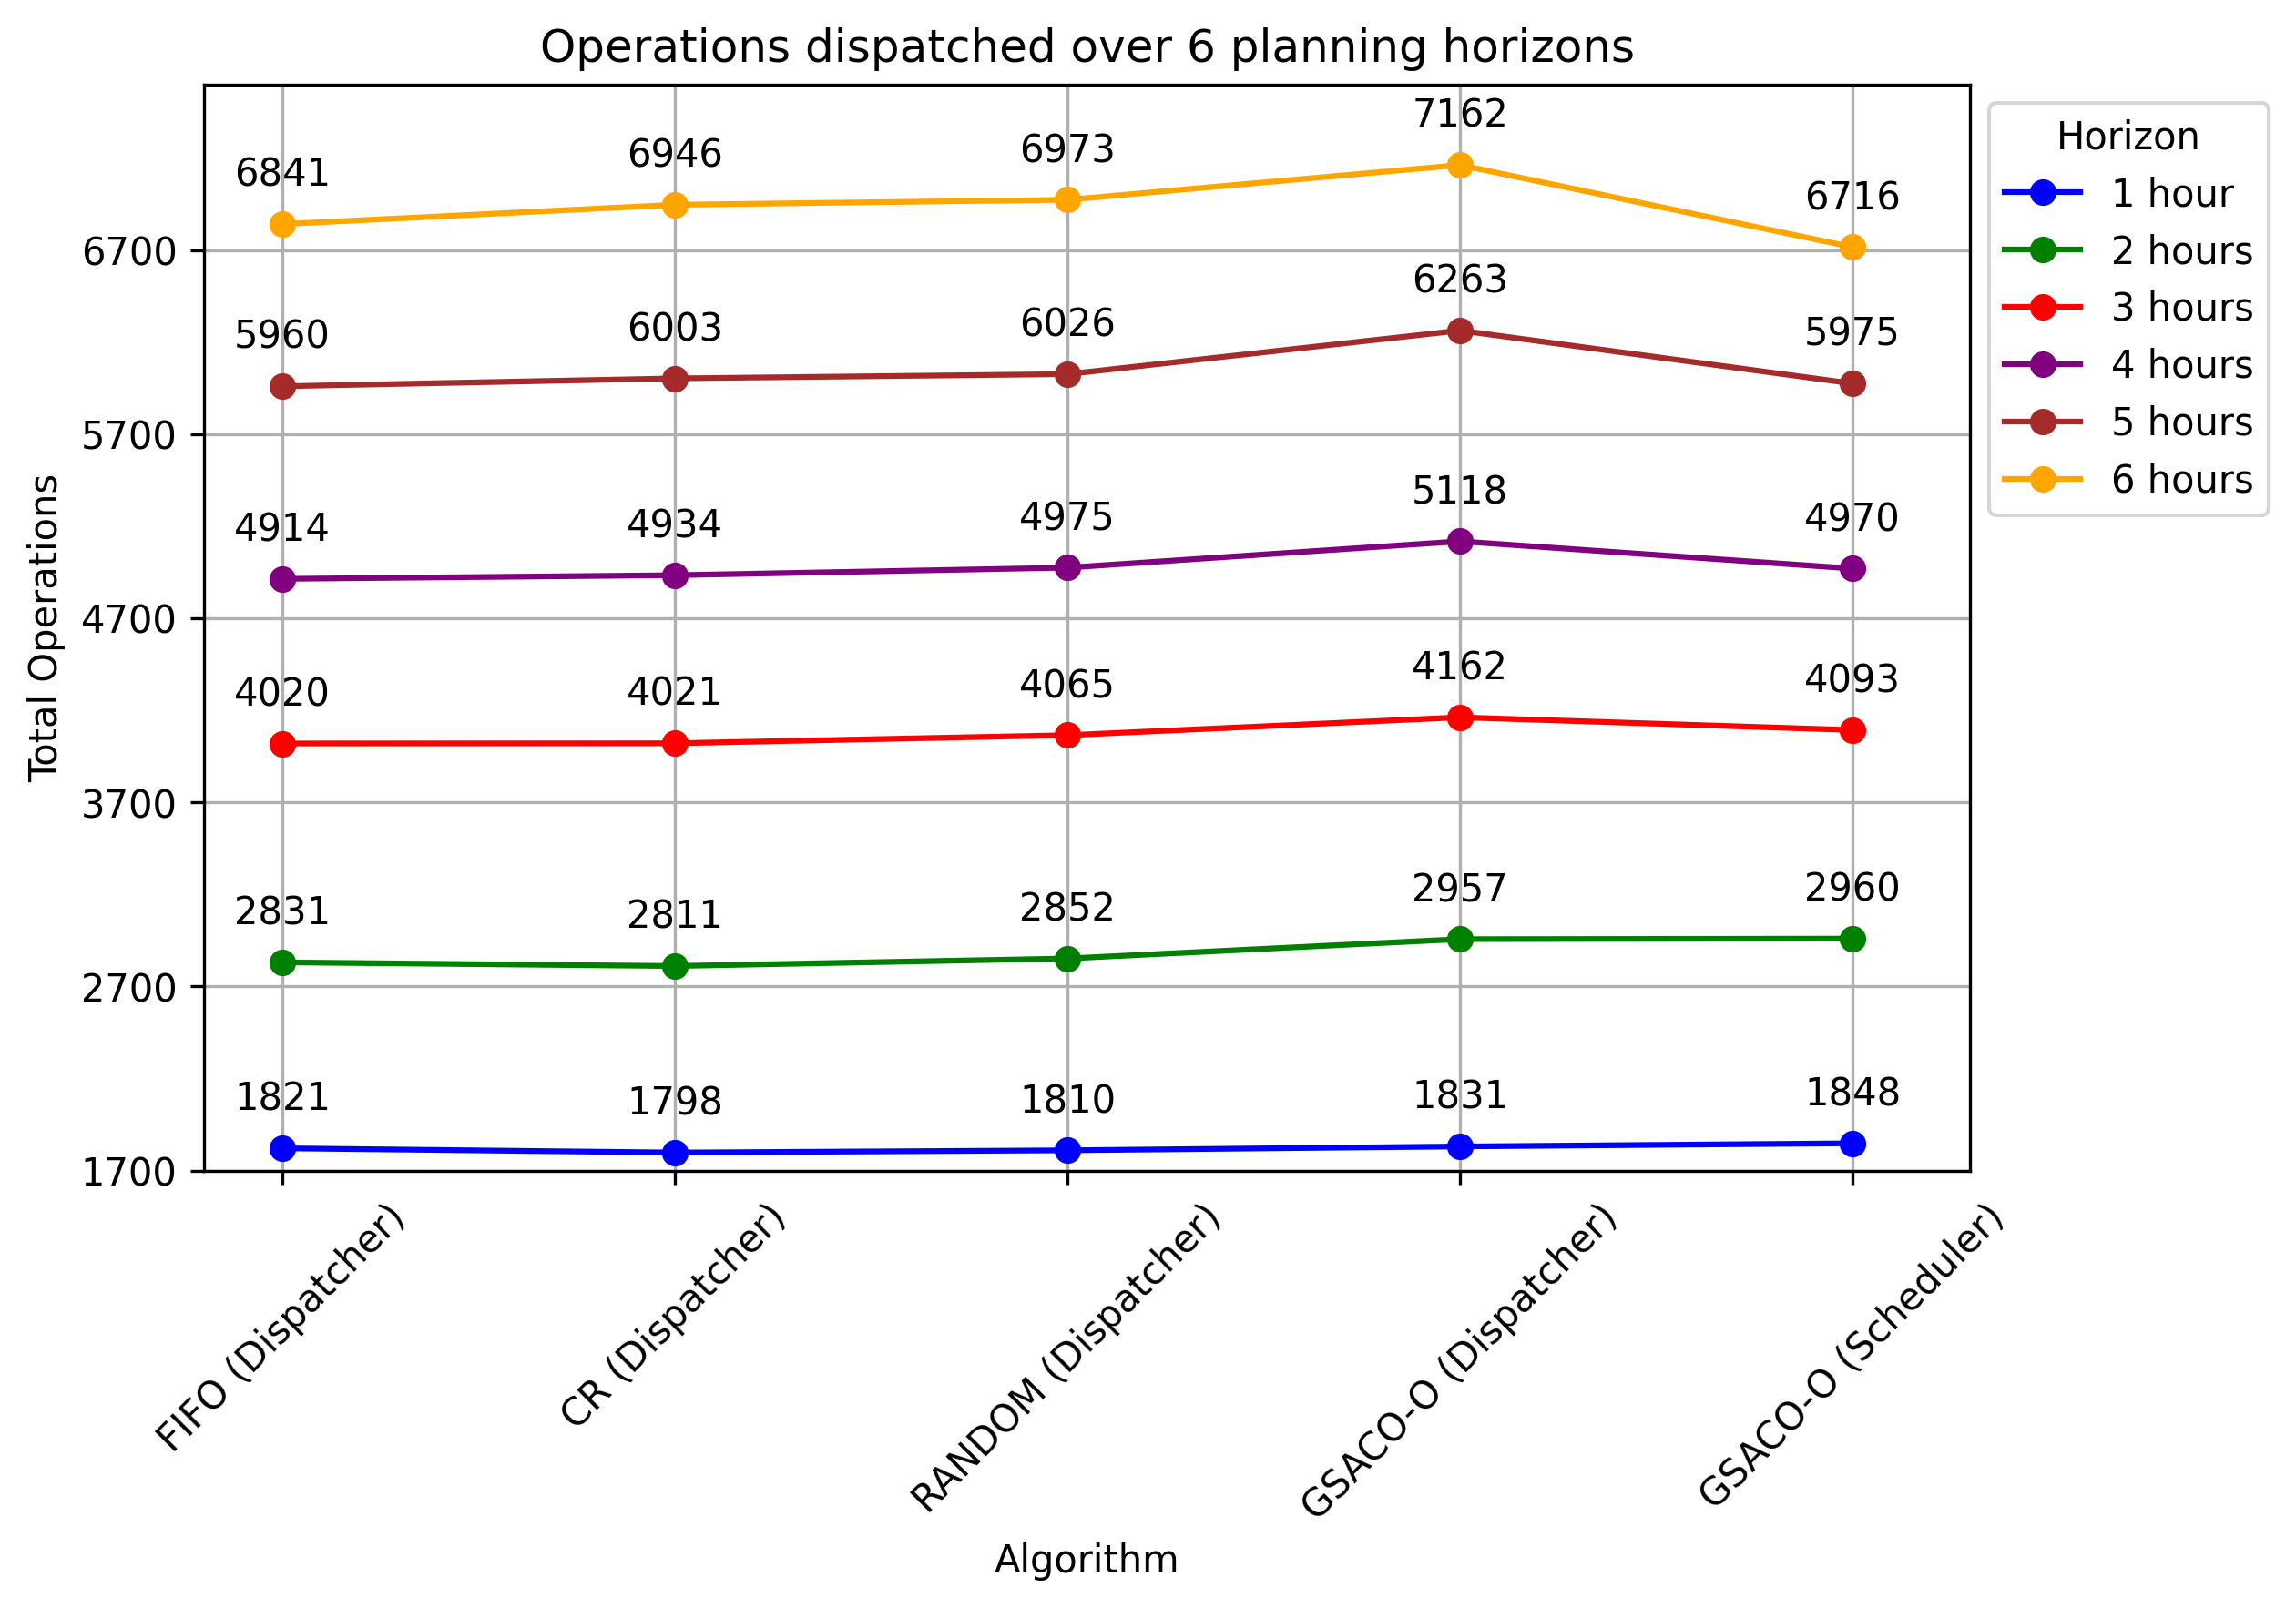
\includegraphics[width=\textwidth]{HVLM/operations_HVLM.png}
	\caption{Operations throughput (HV/LM)}
	\label{fig:totalopsHVLM}
\end{figure}

In Figure~\ref{fig:totalopsLVHM} and Figure~\ref{fig:totalopsHVLM}, the performance of dispatching rules; FIFO, CR, RANDOM, GSACO-O and GSACO-O as scheduler across different planning horizons ranging from 1 to 6 hours is presented. Each plot illustrates the total number of operations dispatched by each rule within these time frames, offering a clear comparison of their efficiency and effectiveness in handling operational tasks within a semiconductor manufacturing.


\begin{figure}[t]
	\centering
	\begin{subfigure}{0.32\textwidth}
		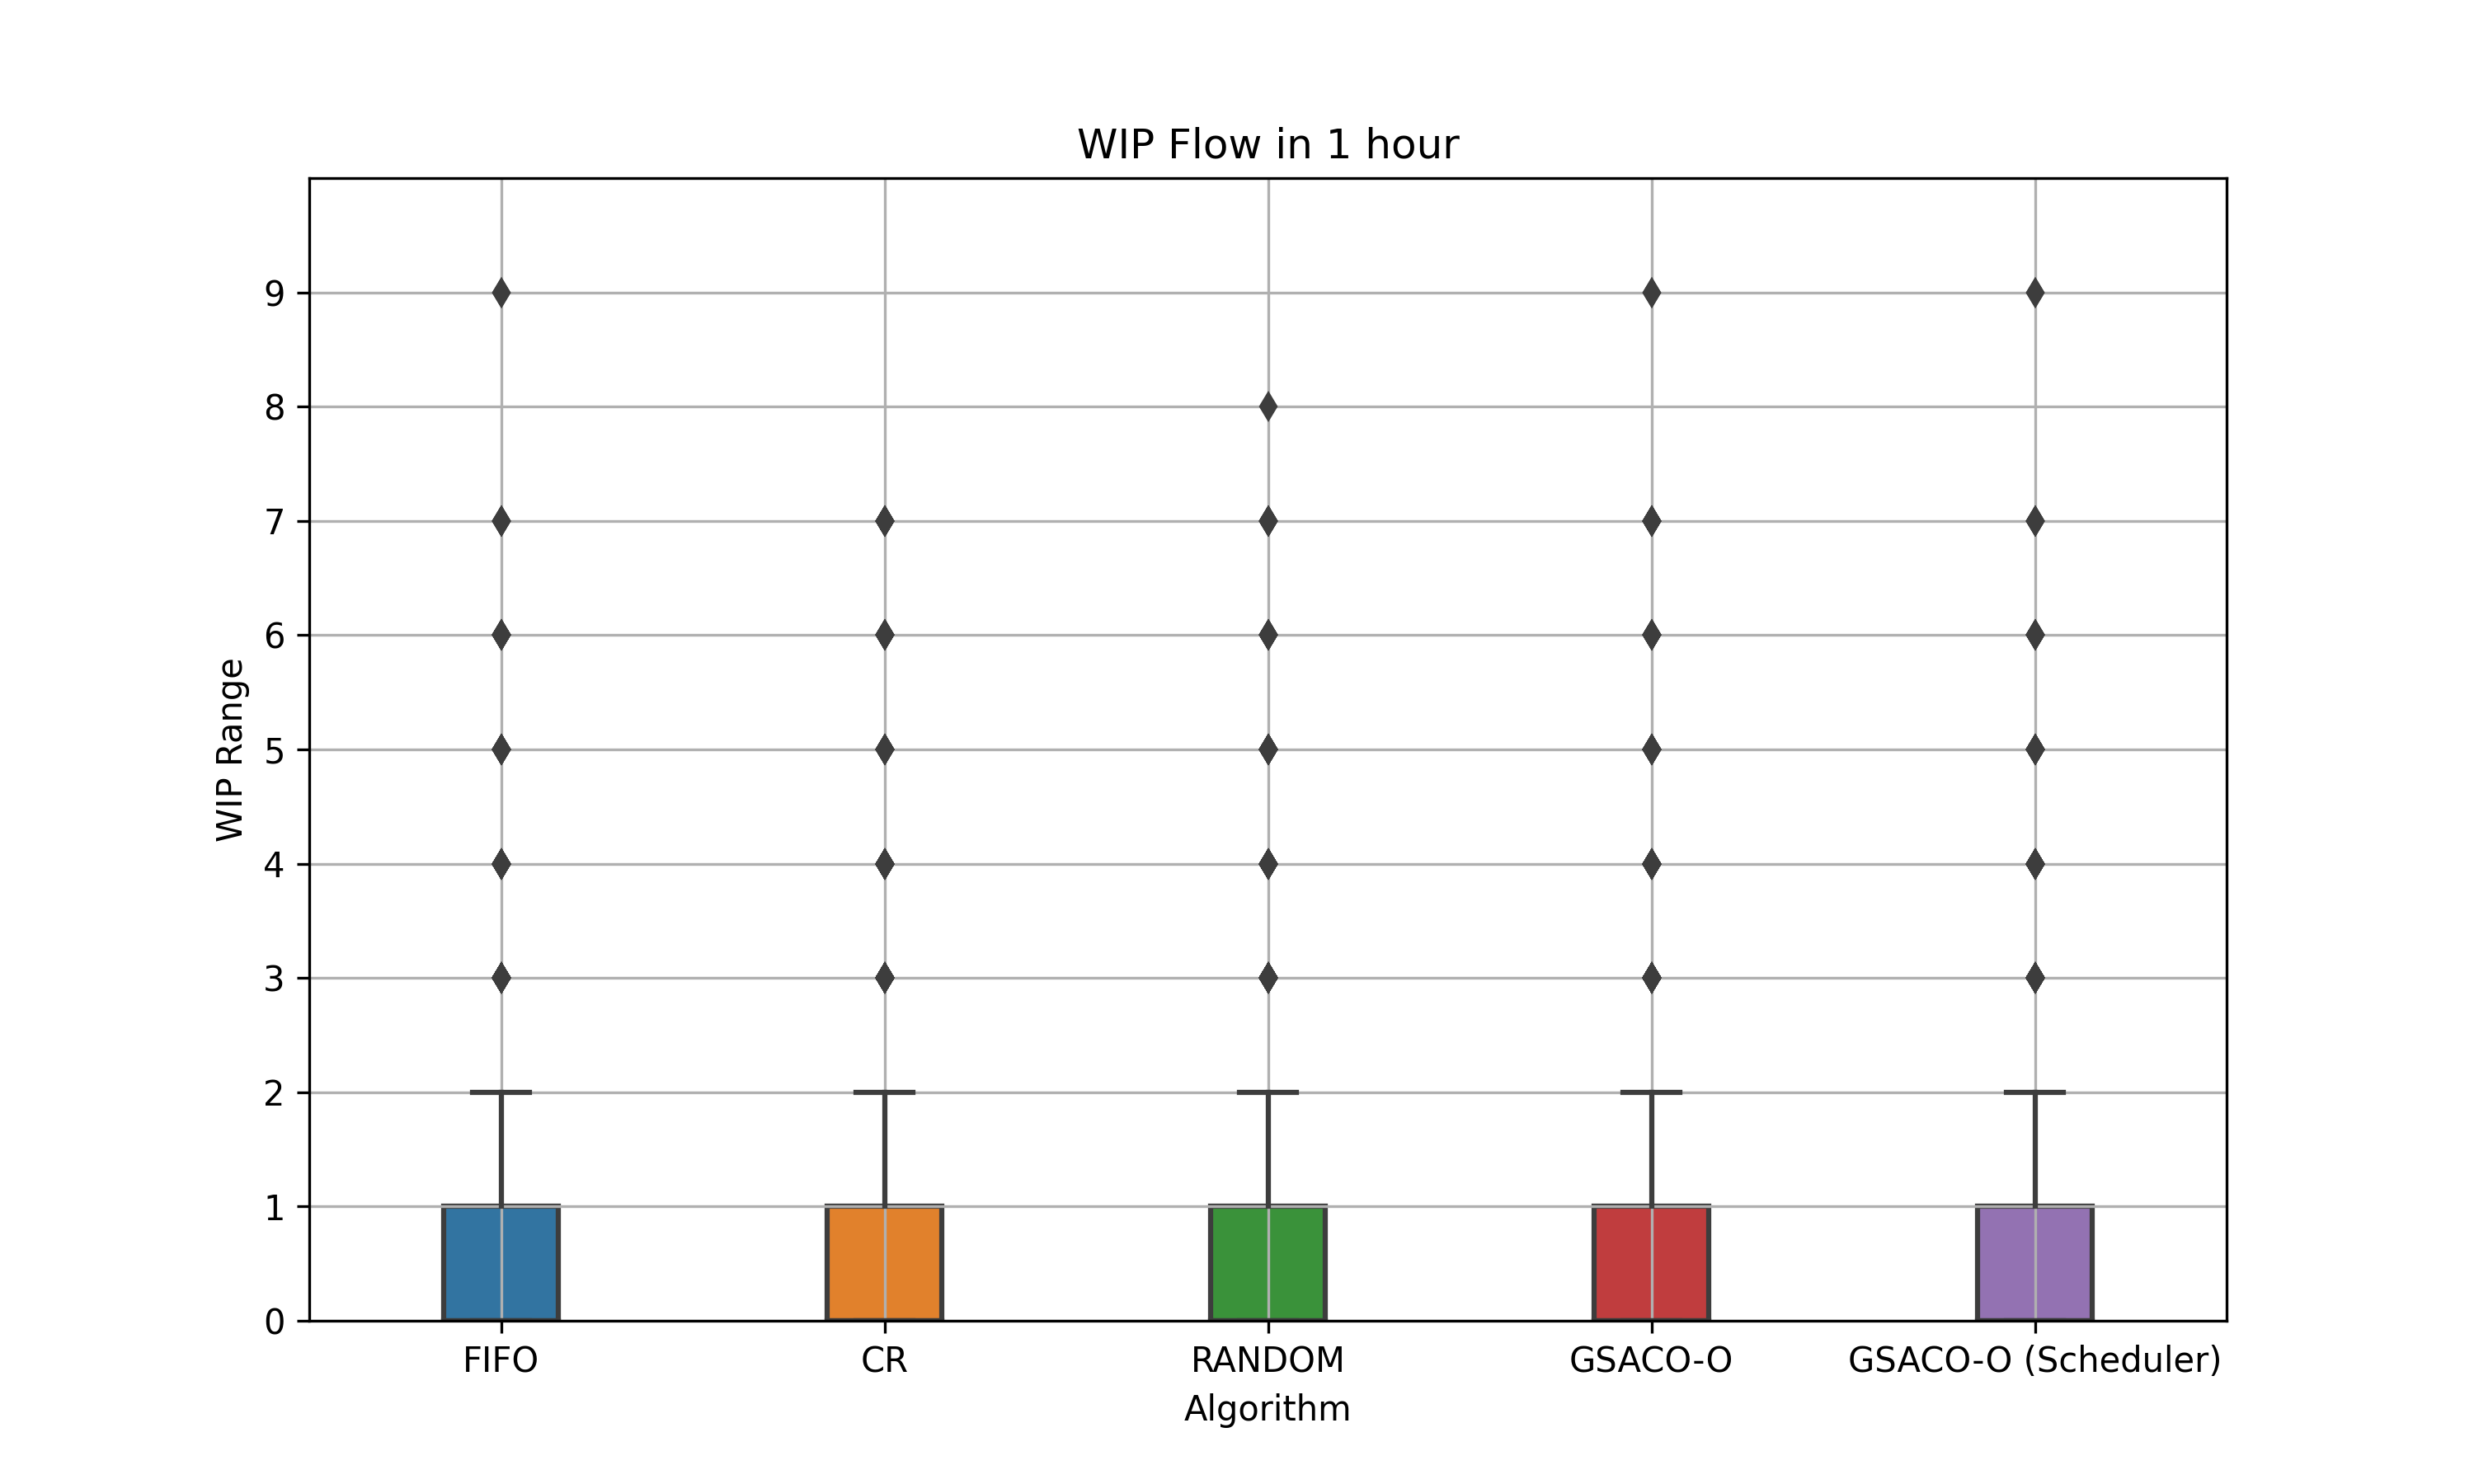
\includegraphics[width=\textwidth]{LVHM/new_period_3600s.png}
		% \caption{}
		% \label{fig:pp1}
	\end{subfigure}\hfill
	\begin{subfigure}{0.32\textwidth}
		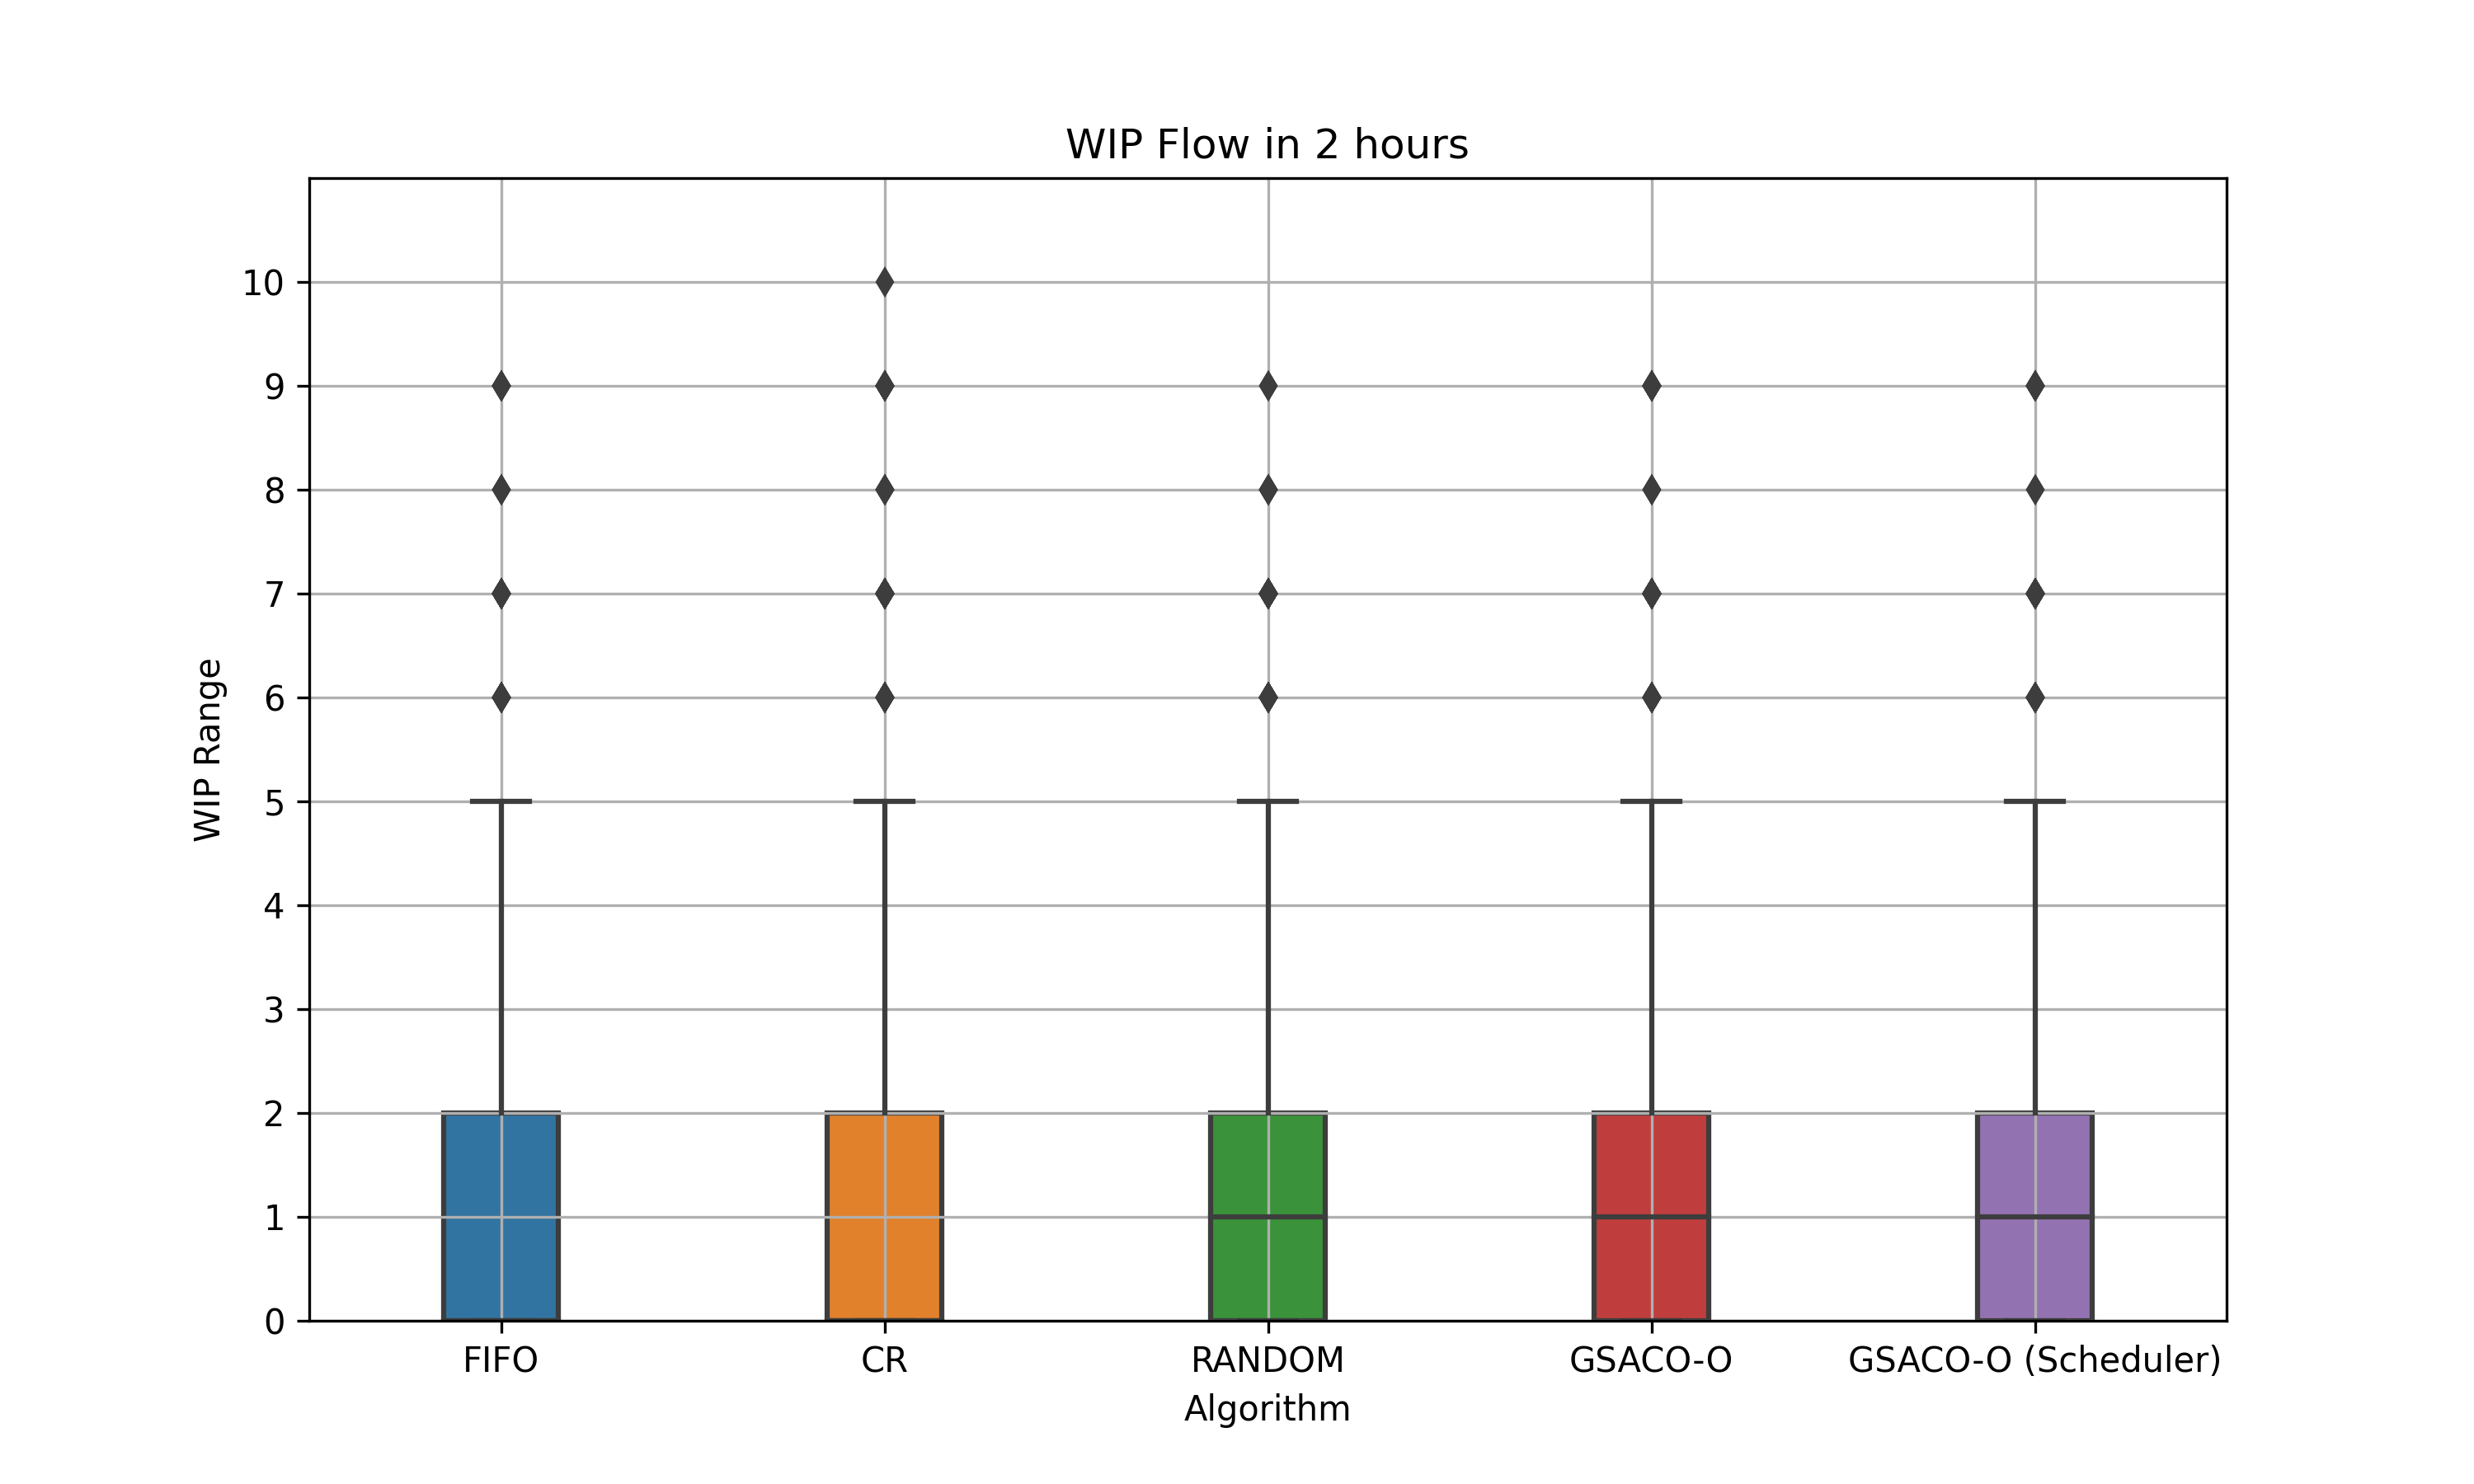
\includegraphics[width=\textwidth]{LVHM/new_period_7200s.png}
		% \caption{}
		% \label{fig:pp2}
	\end{subfigure}\hfill
	\begin{subfigure}{0.32\textwidth}
		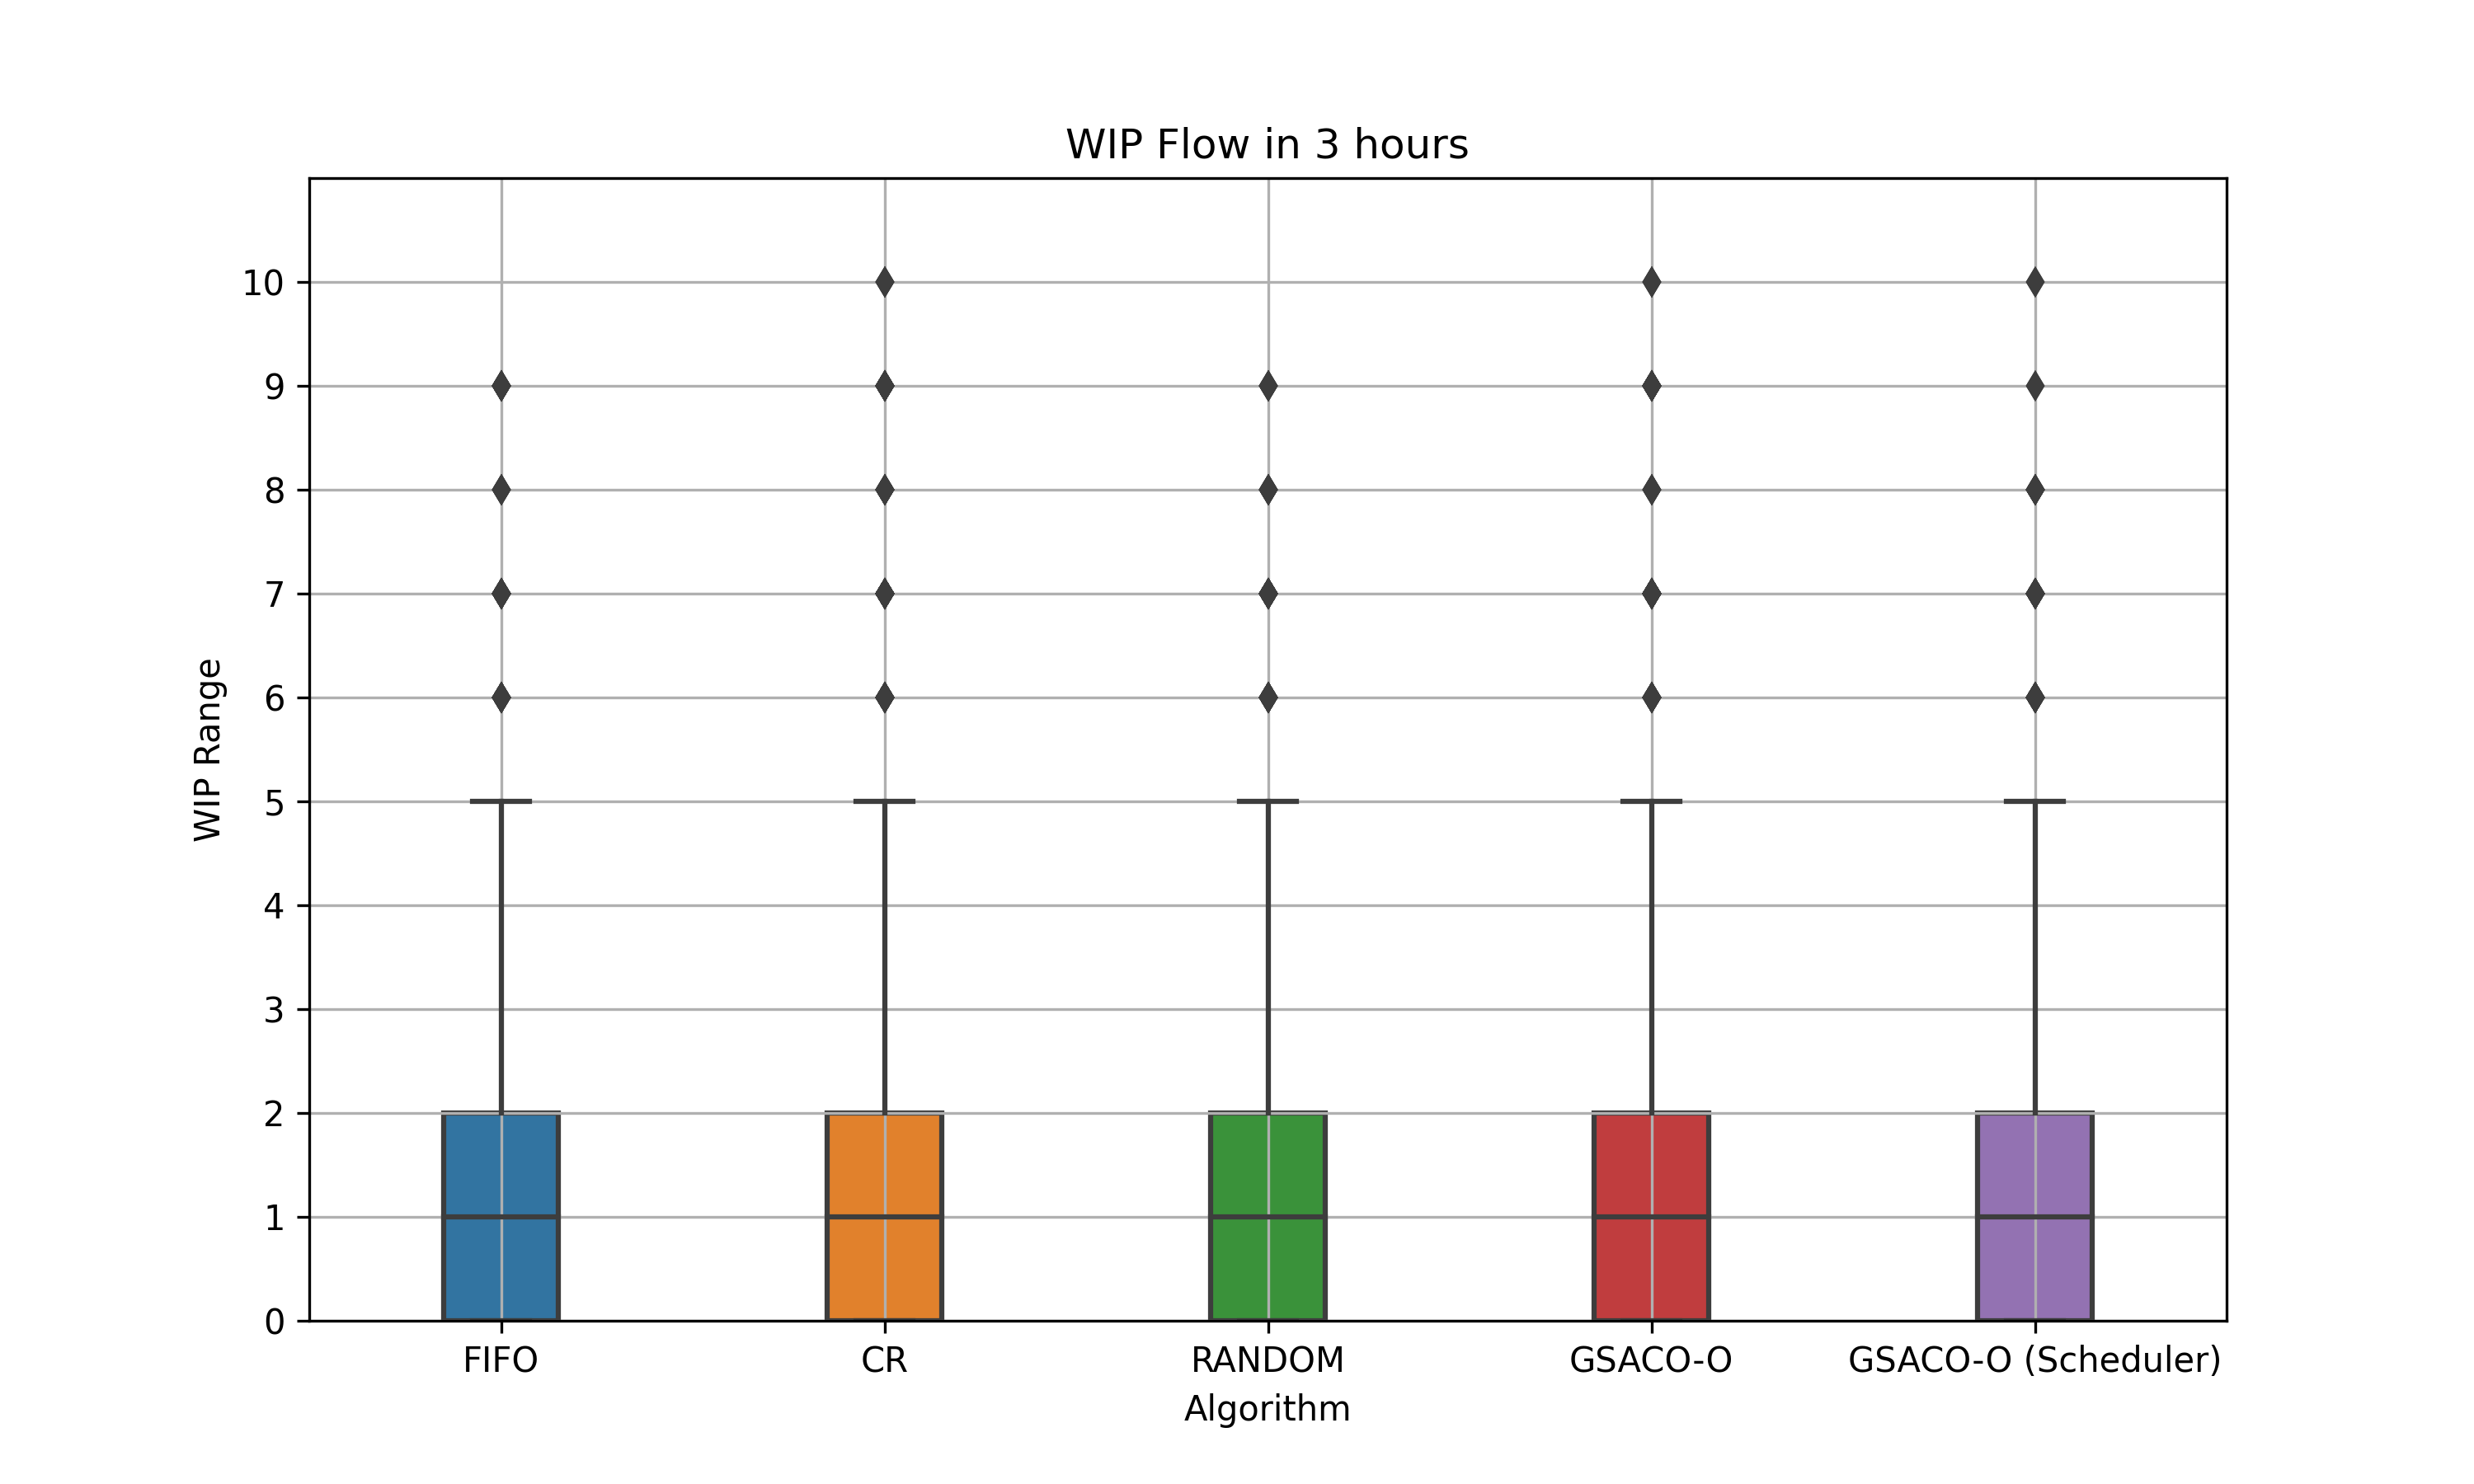
\includegraphics[width=\textwidth]{LVHM/new_period_10800s.png}
		% \caption{}
		% \label{fig:pp3}
	\end{subfigure}
	\begin{subfigure}{0.32\textwidth}
		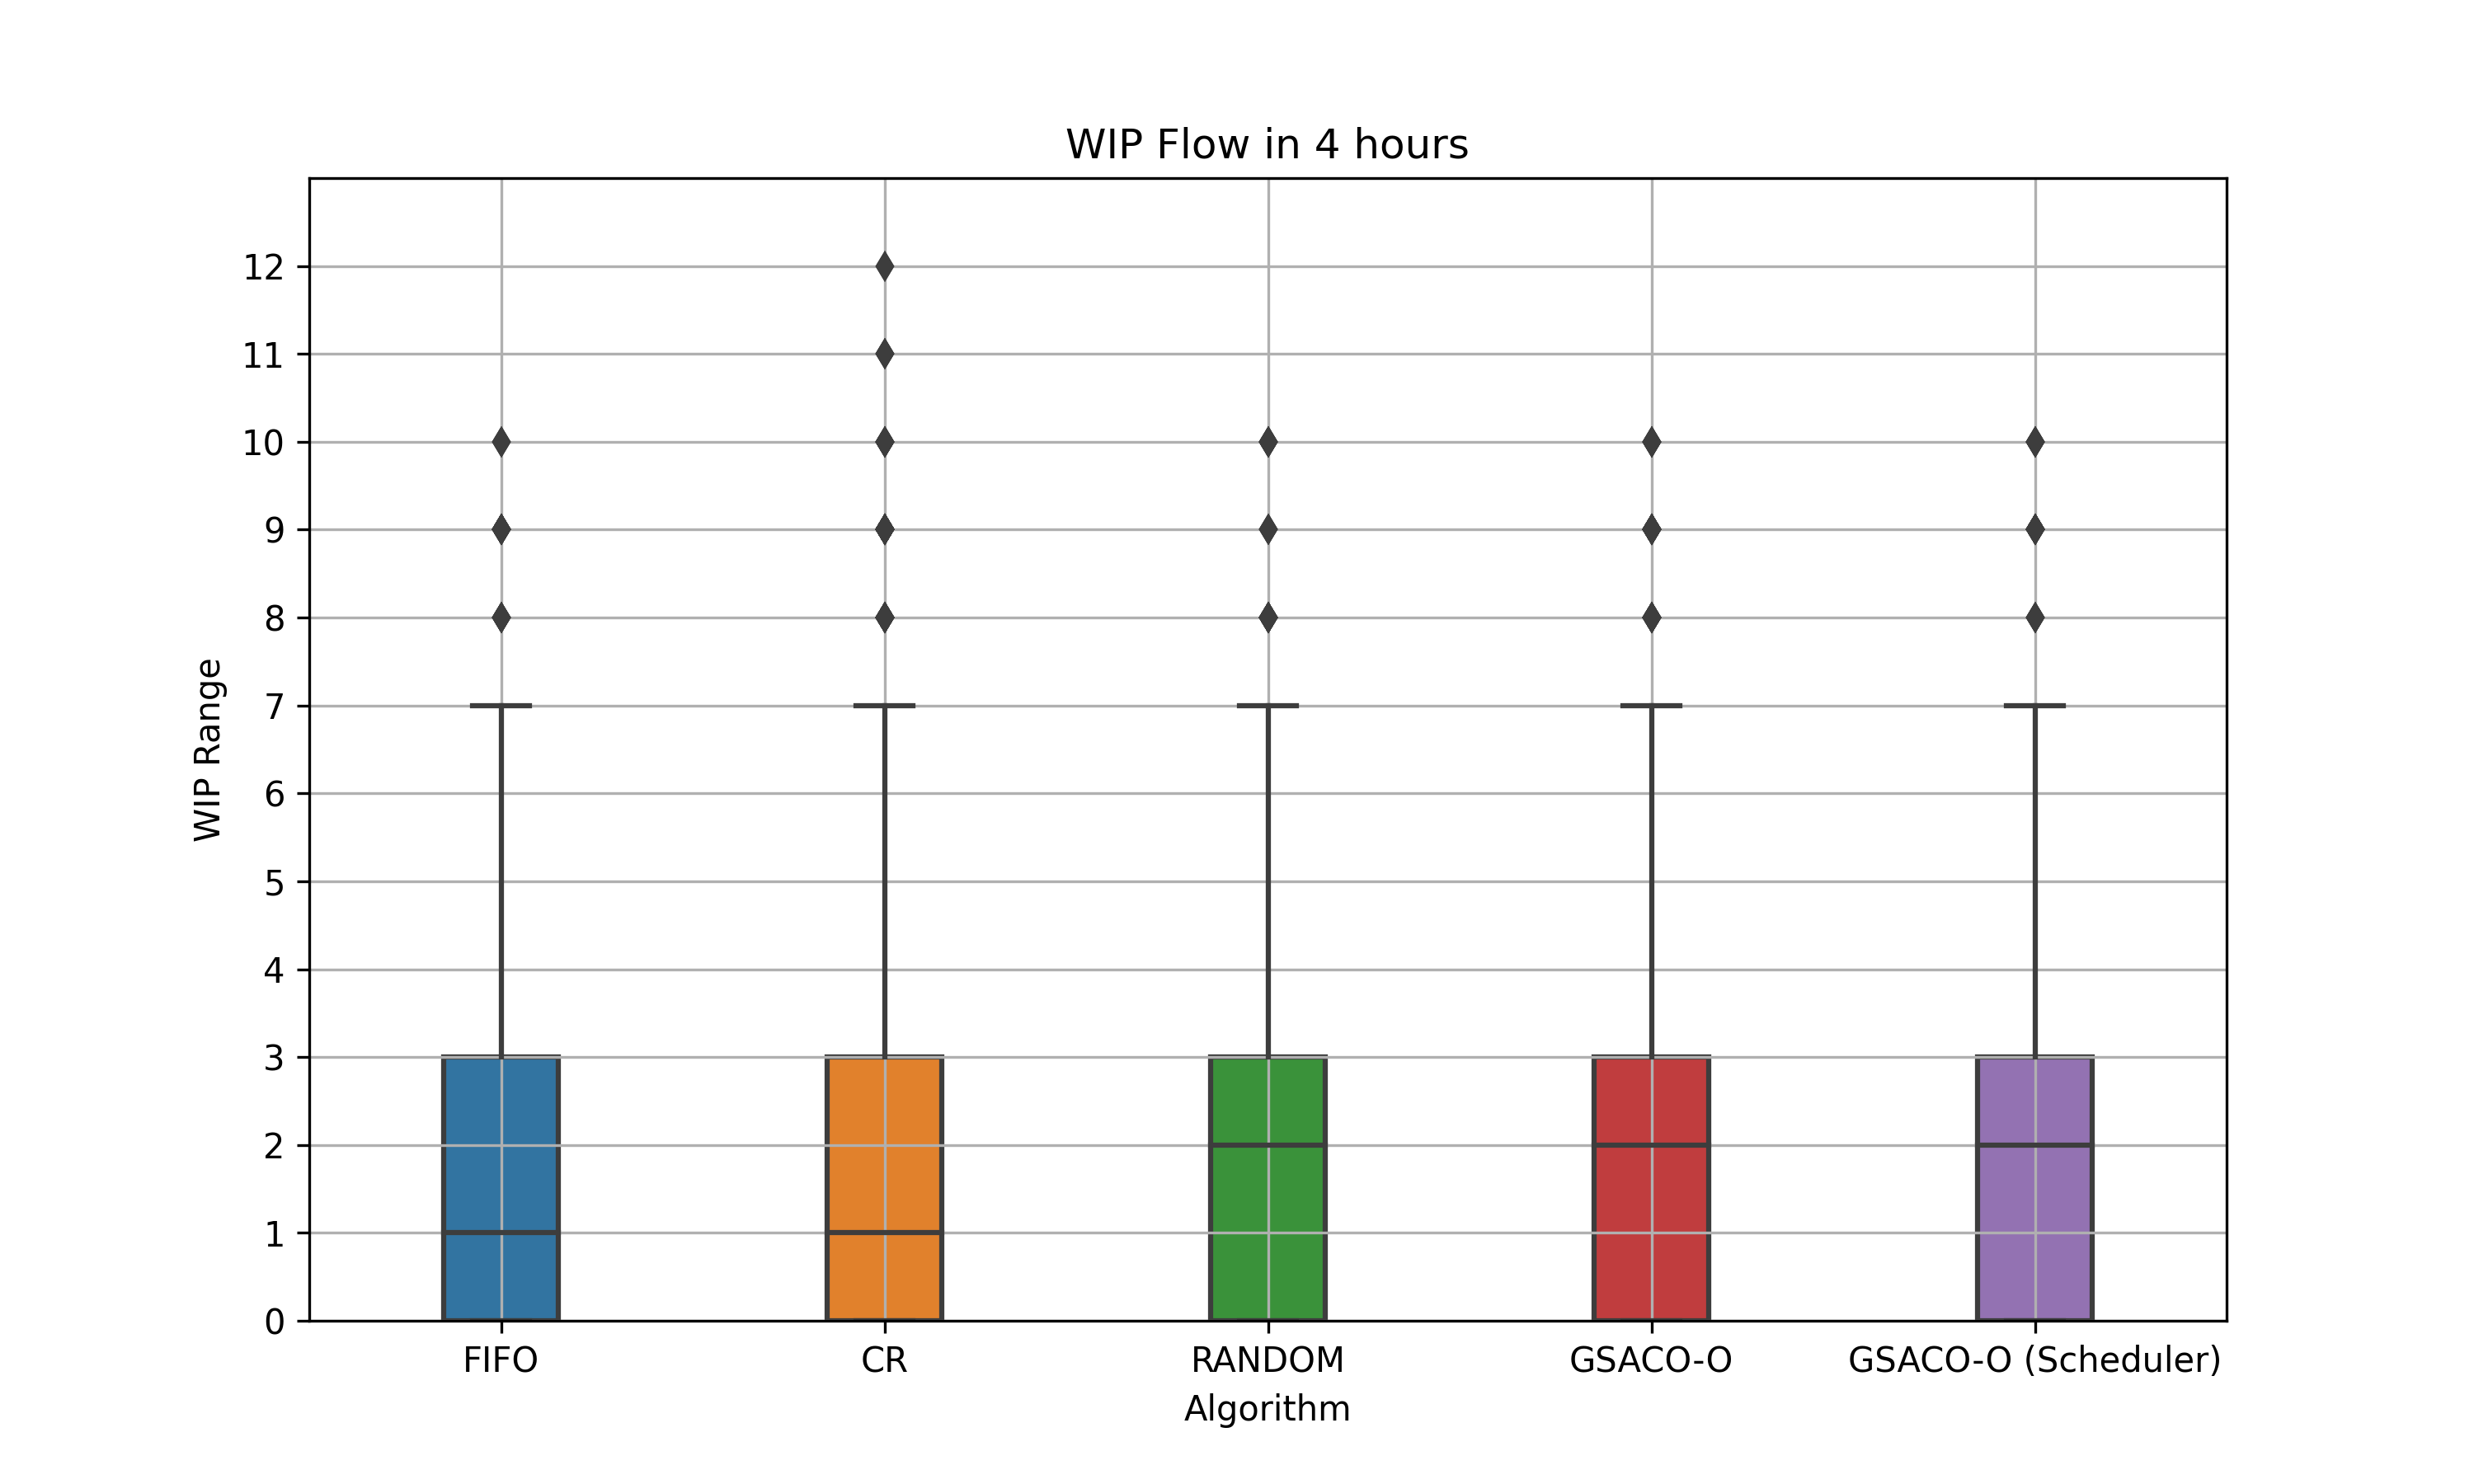
\includegraphics[width=\textwidth]{LVHM/new_period_14400s.png}
		% \caption{}
		% \label{fig:pp4}
	\end{subfigure}\hfill
	\begin{subfigure}{0.32\textwidth}
		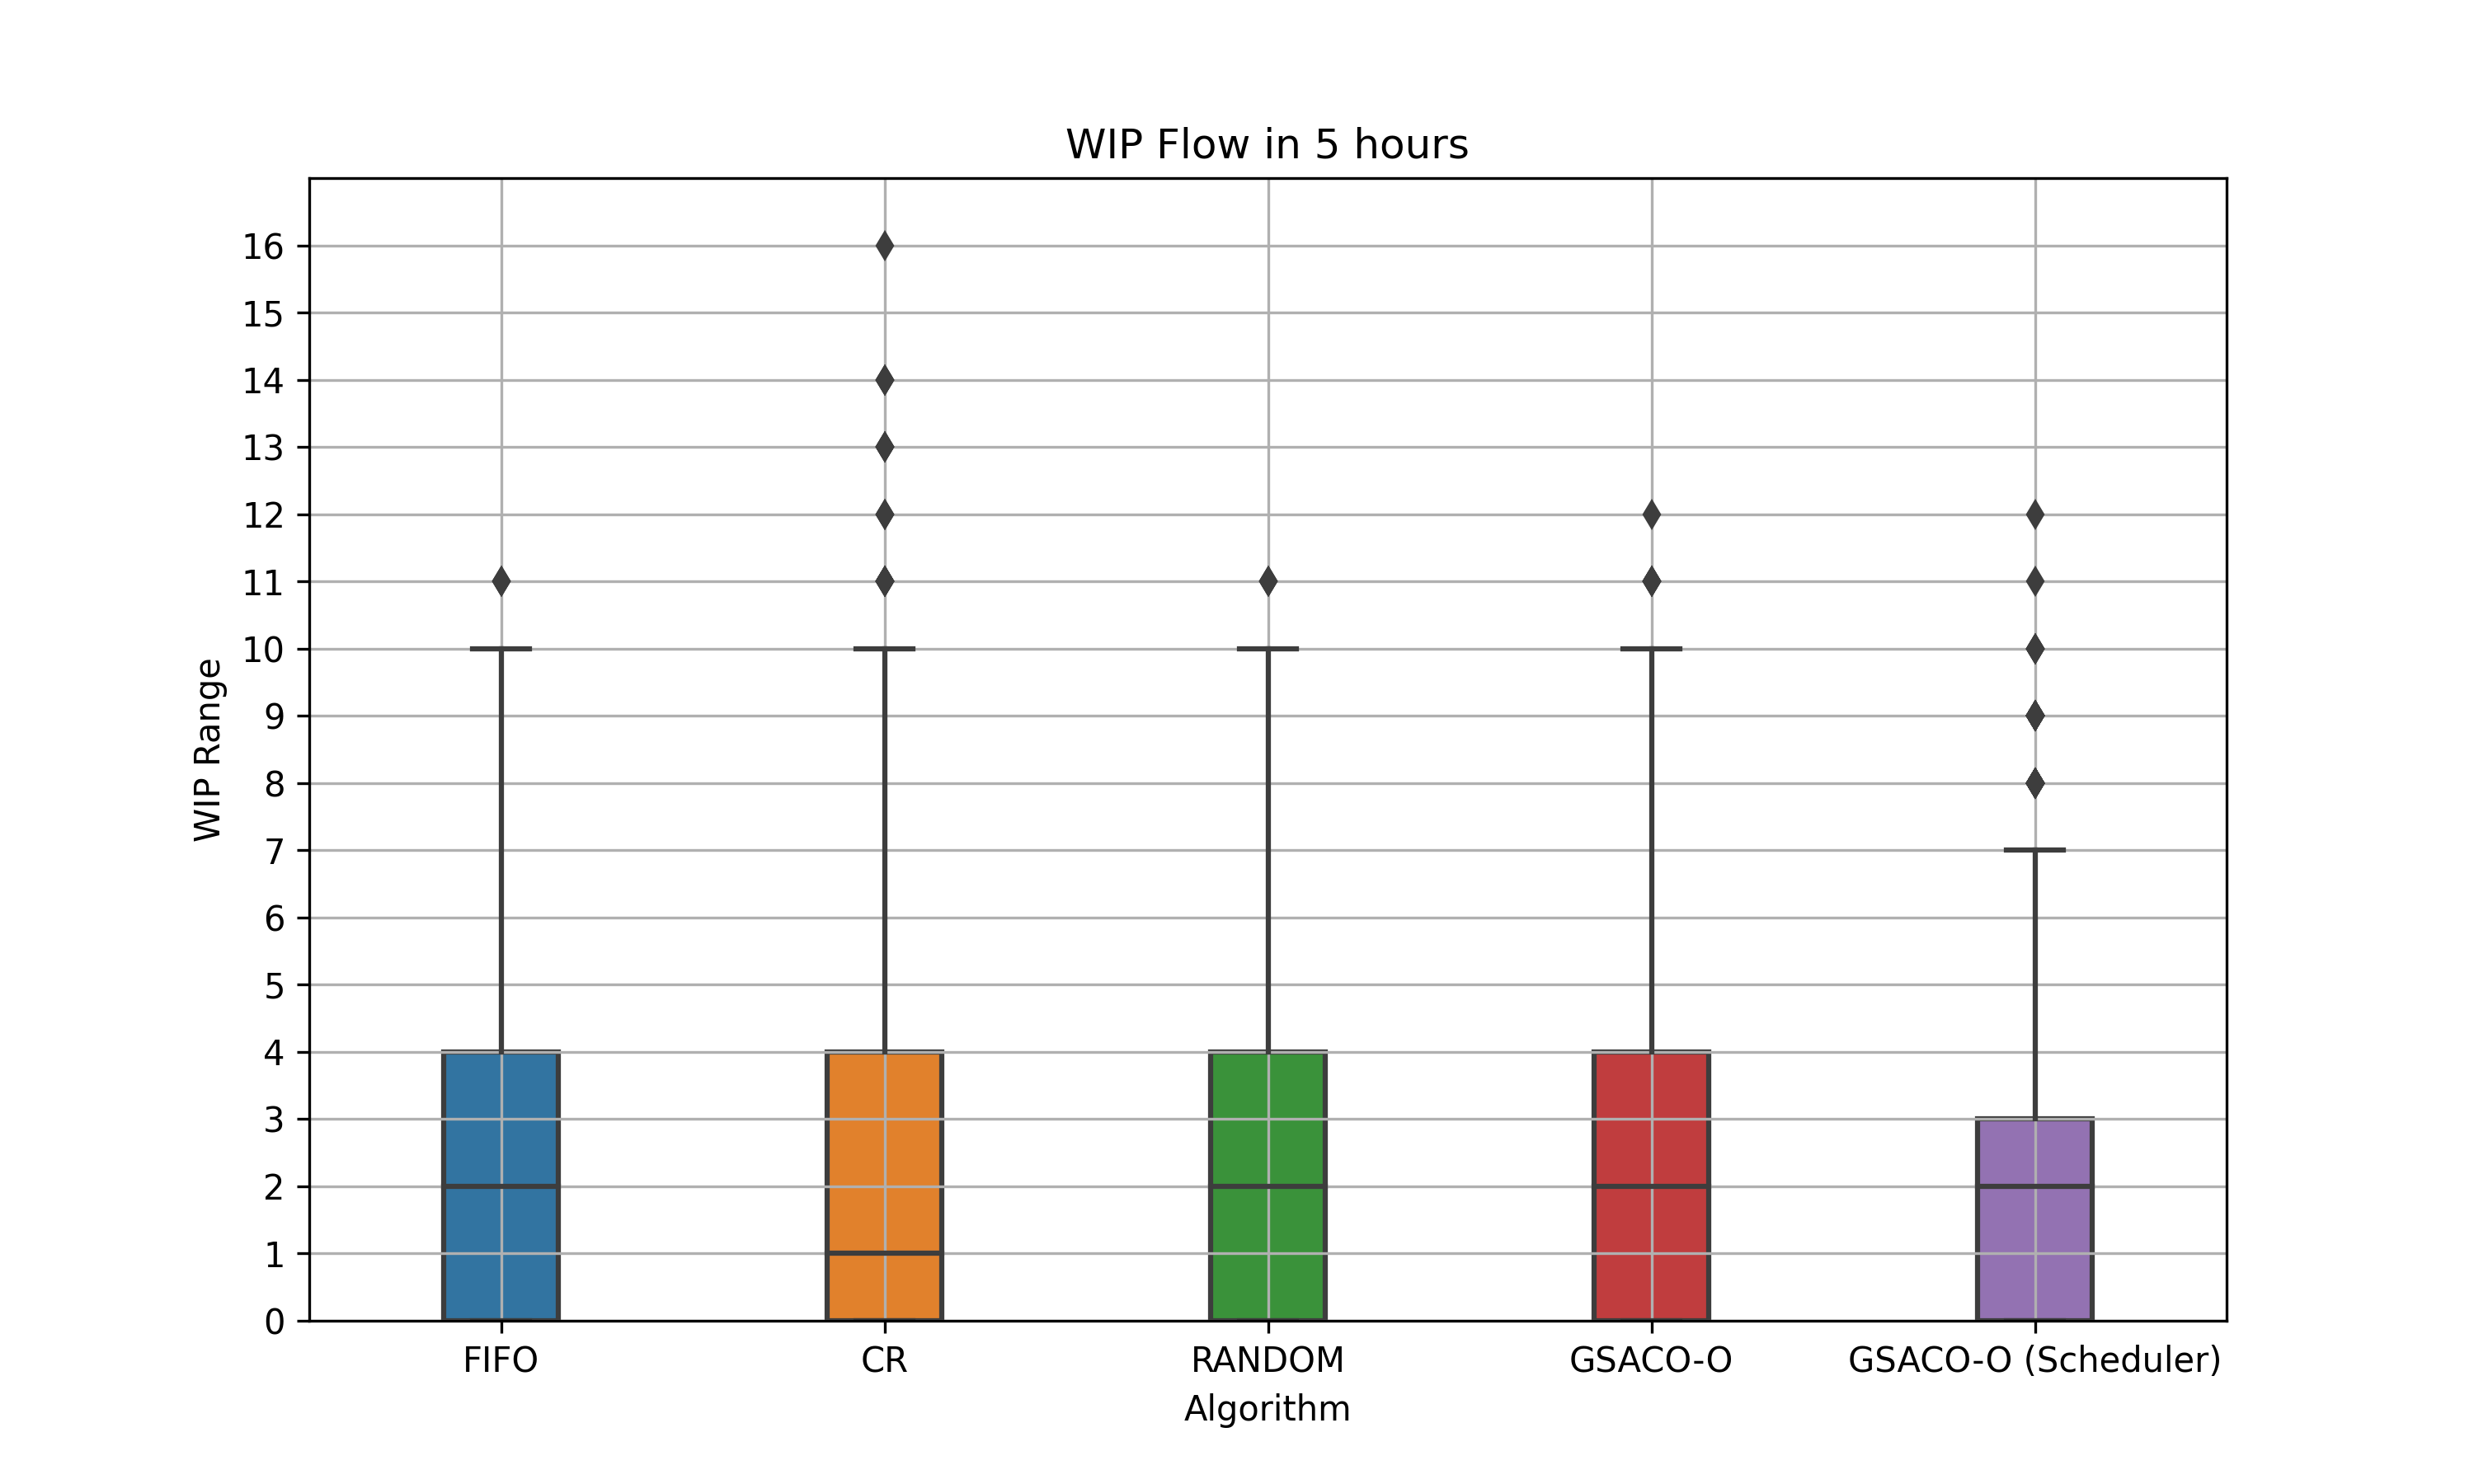
\includegraphics[width=\textwidth]{LVHM/new_period_18000s.png}
		% \caption{}
		% \label{fig:pp5}
	\end{subfigure}\hfill
	\begin{subfigure}{0.32\textwidth}
		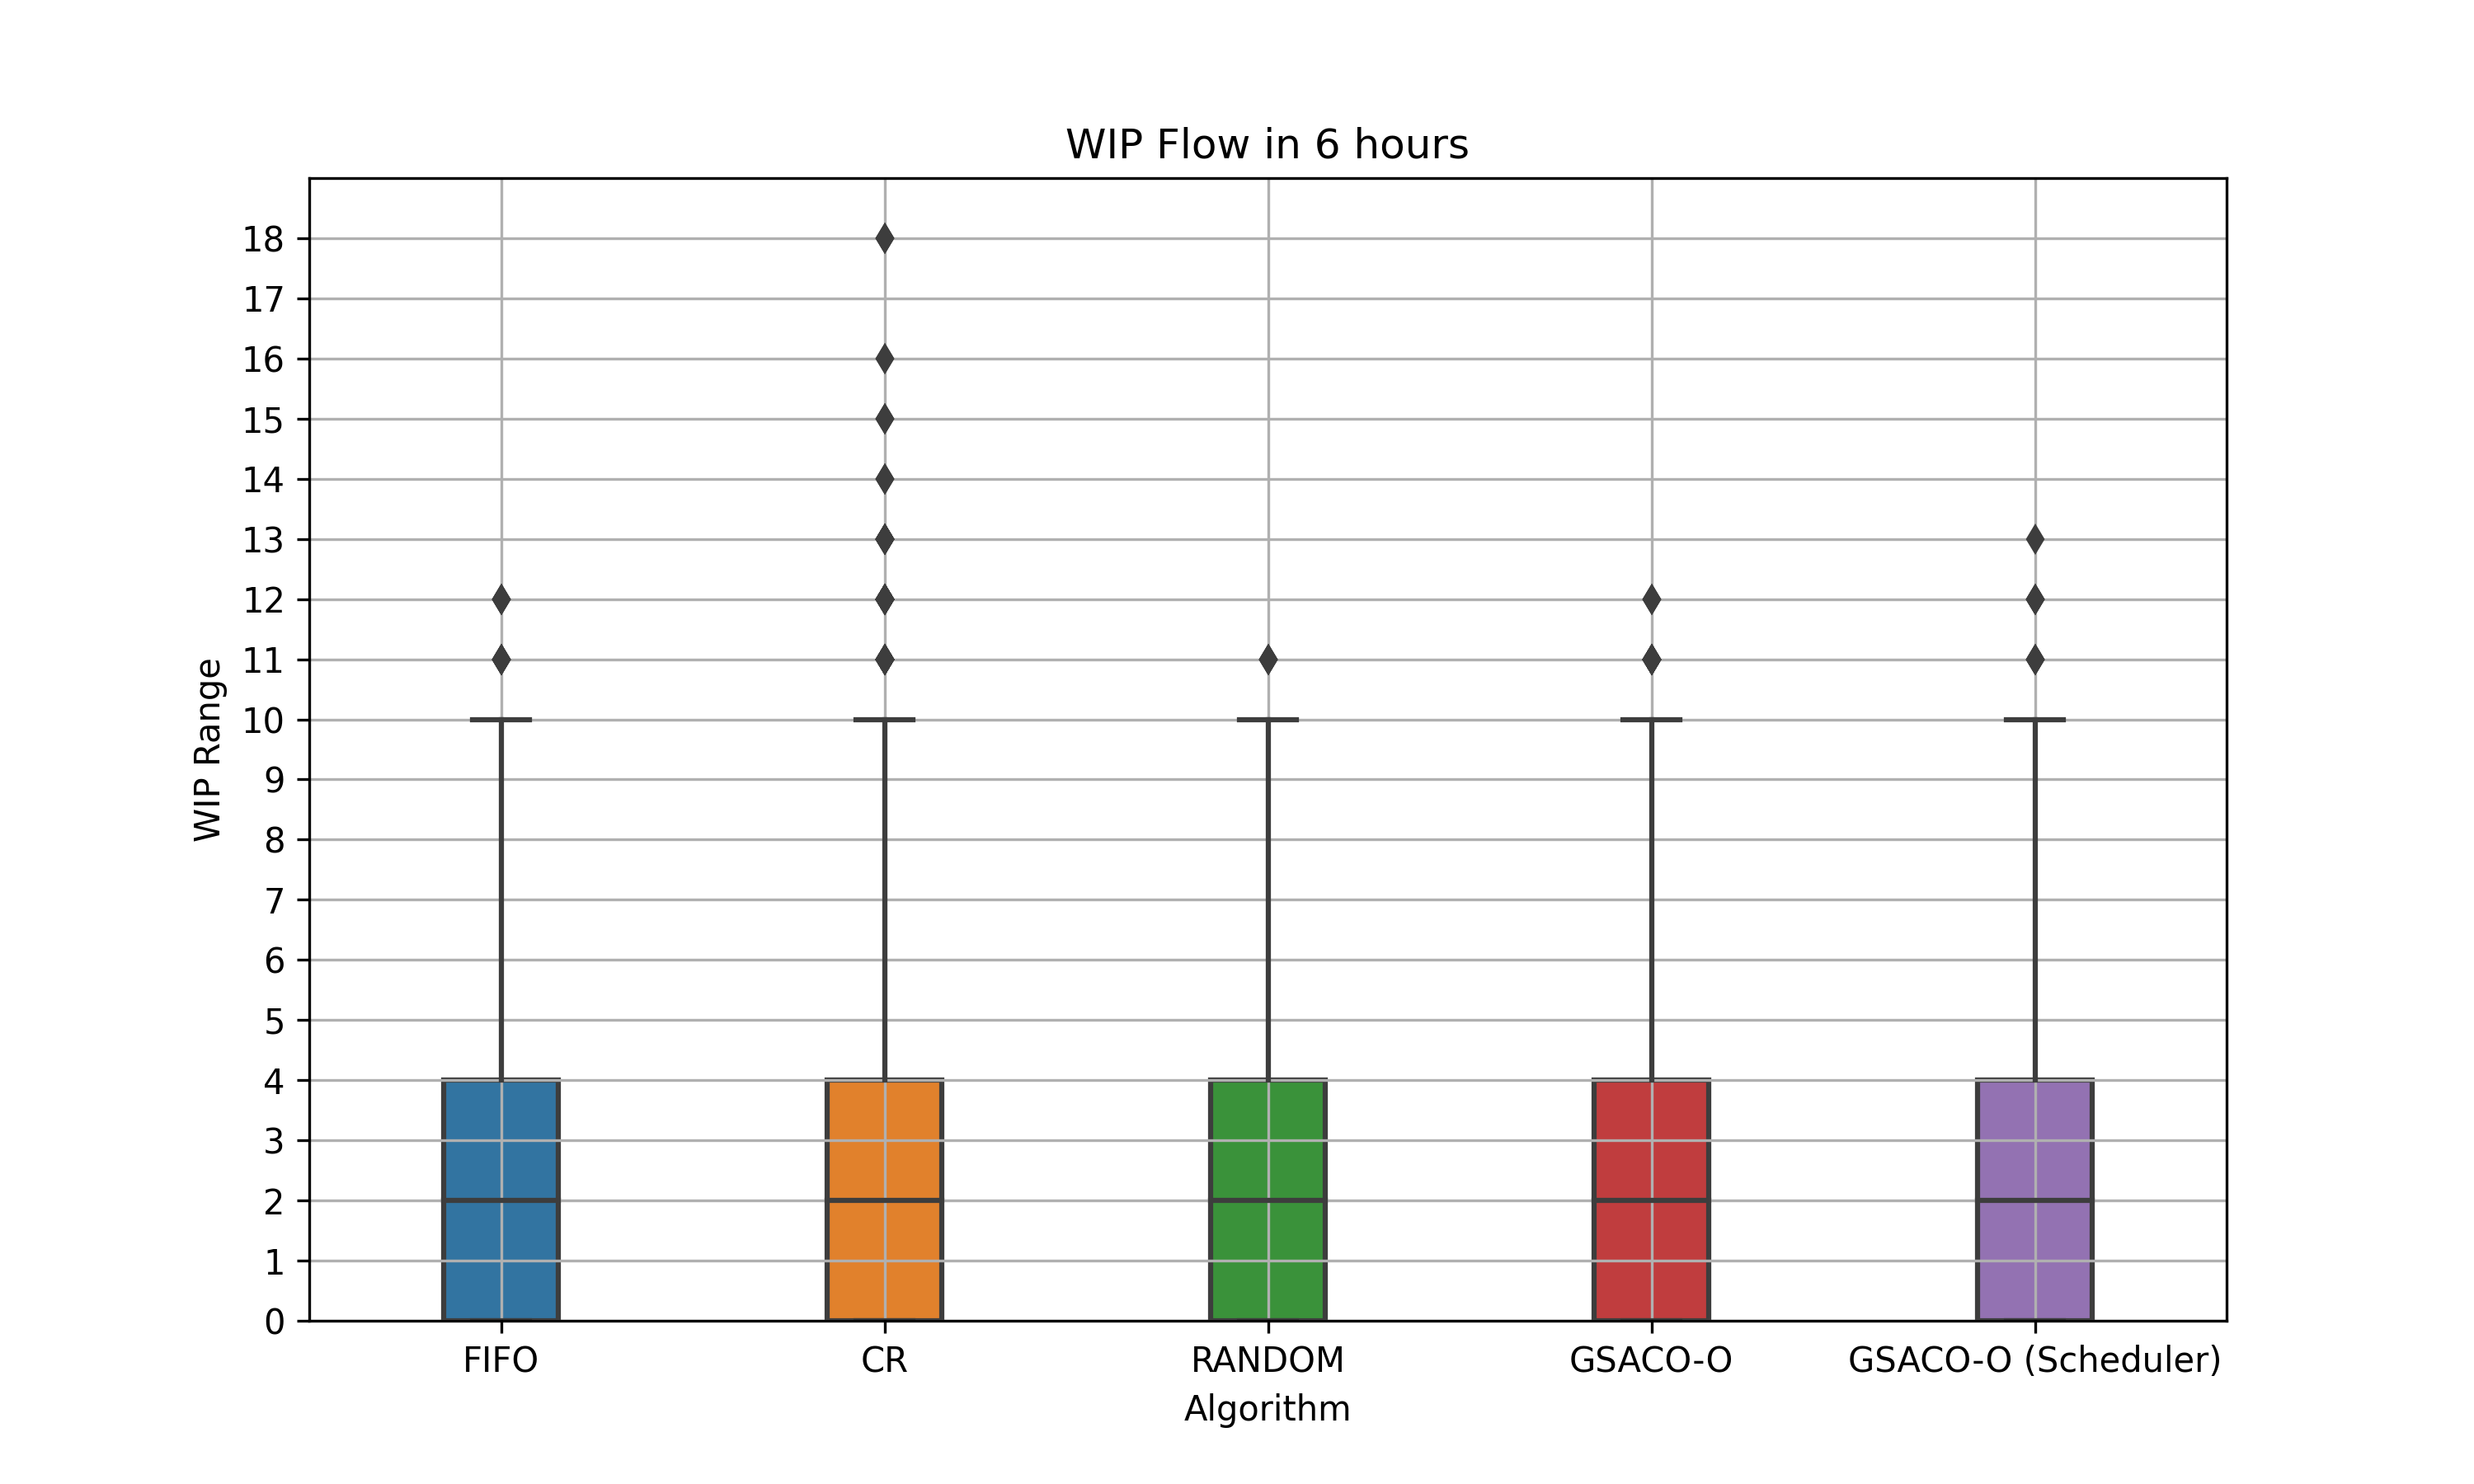
\includegraphics[width=\textwidth]{LVHM/new_period_21600s.png}
		% \caption{}
		% \label{fig:pp6}
	\end{subfigure}
    \caption{WIP flow for LV/HM}
    \label{fig:wip-flows-LVHM}
\end{figure}

The plots in Figure~\ref{fig:wip-flows-LVHM} illustrate the Work-in-Progress (WIP) flow for the LV/HM scenario across various dispatching rules FIFO, CR, RANDOM, GSACO-O, and GSACO-O as scheduler over different planning horizons ranging from 1 to 6 hours. Each bar demonstrates the minimum and maximum WIP levels reached during the simulation period under each dispatching rule, with the height of the bar indicating the variability or stability of the WIP flow. 
Across all planning horizons, the range of WIP counts is quite consistent across different dispatchers, as represented by FIFO, CR, RANDOM, GSACO-O, and GSACO-O (Scheduler). This suggests that no single dispatcher has a significantly larger WIP range, indicating a balanced approach to managing WIP levels over time.
In case of dispatcher specific observation, FIFO shows the lowest range of WIP variability, suggesting consistent and predictable processing under this rule within the first hour. CR and Random display slightly higher variability, indicating a less stable WIP flow.
Across the longer planning horizons such as 5 and 6 hours, there are more outliers in WIP counts across all dispatchers, which could indicate sporadic spikes in WIP. This trend shows increase in job complexity as the period extends. 
GSACO-O, in both dispatcher and scheduler forms, demonstrates a consistent WIP distribution that does not deviate significantly across time horizons. This indicate that the GSACO-O method is robust in maintaining predictable WIP flows, regardless of operational duration.


\begin{figure}[t]
	\centering
	\begin{subfigure}[b]{0.32\textwidth}
		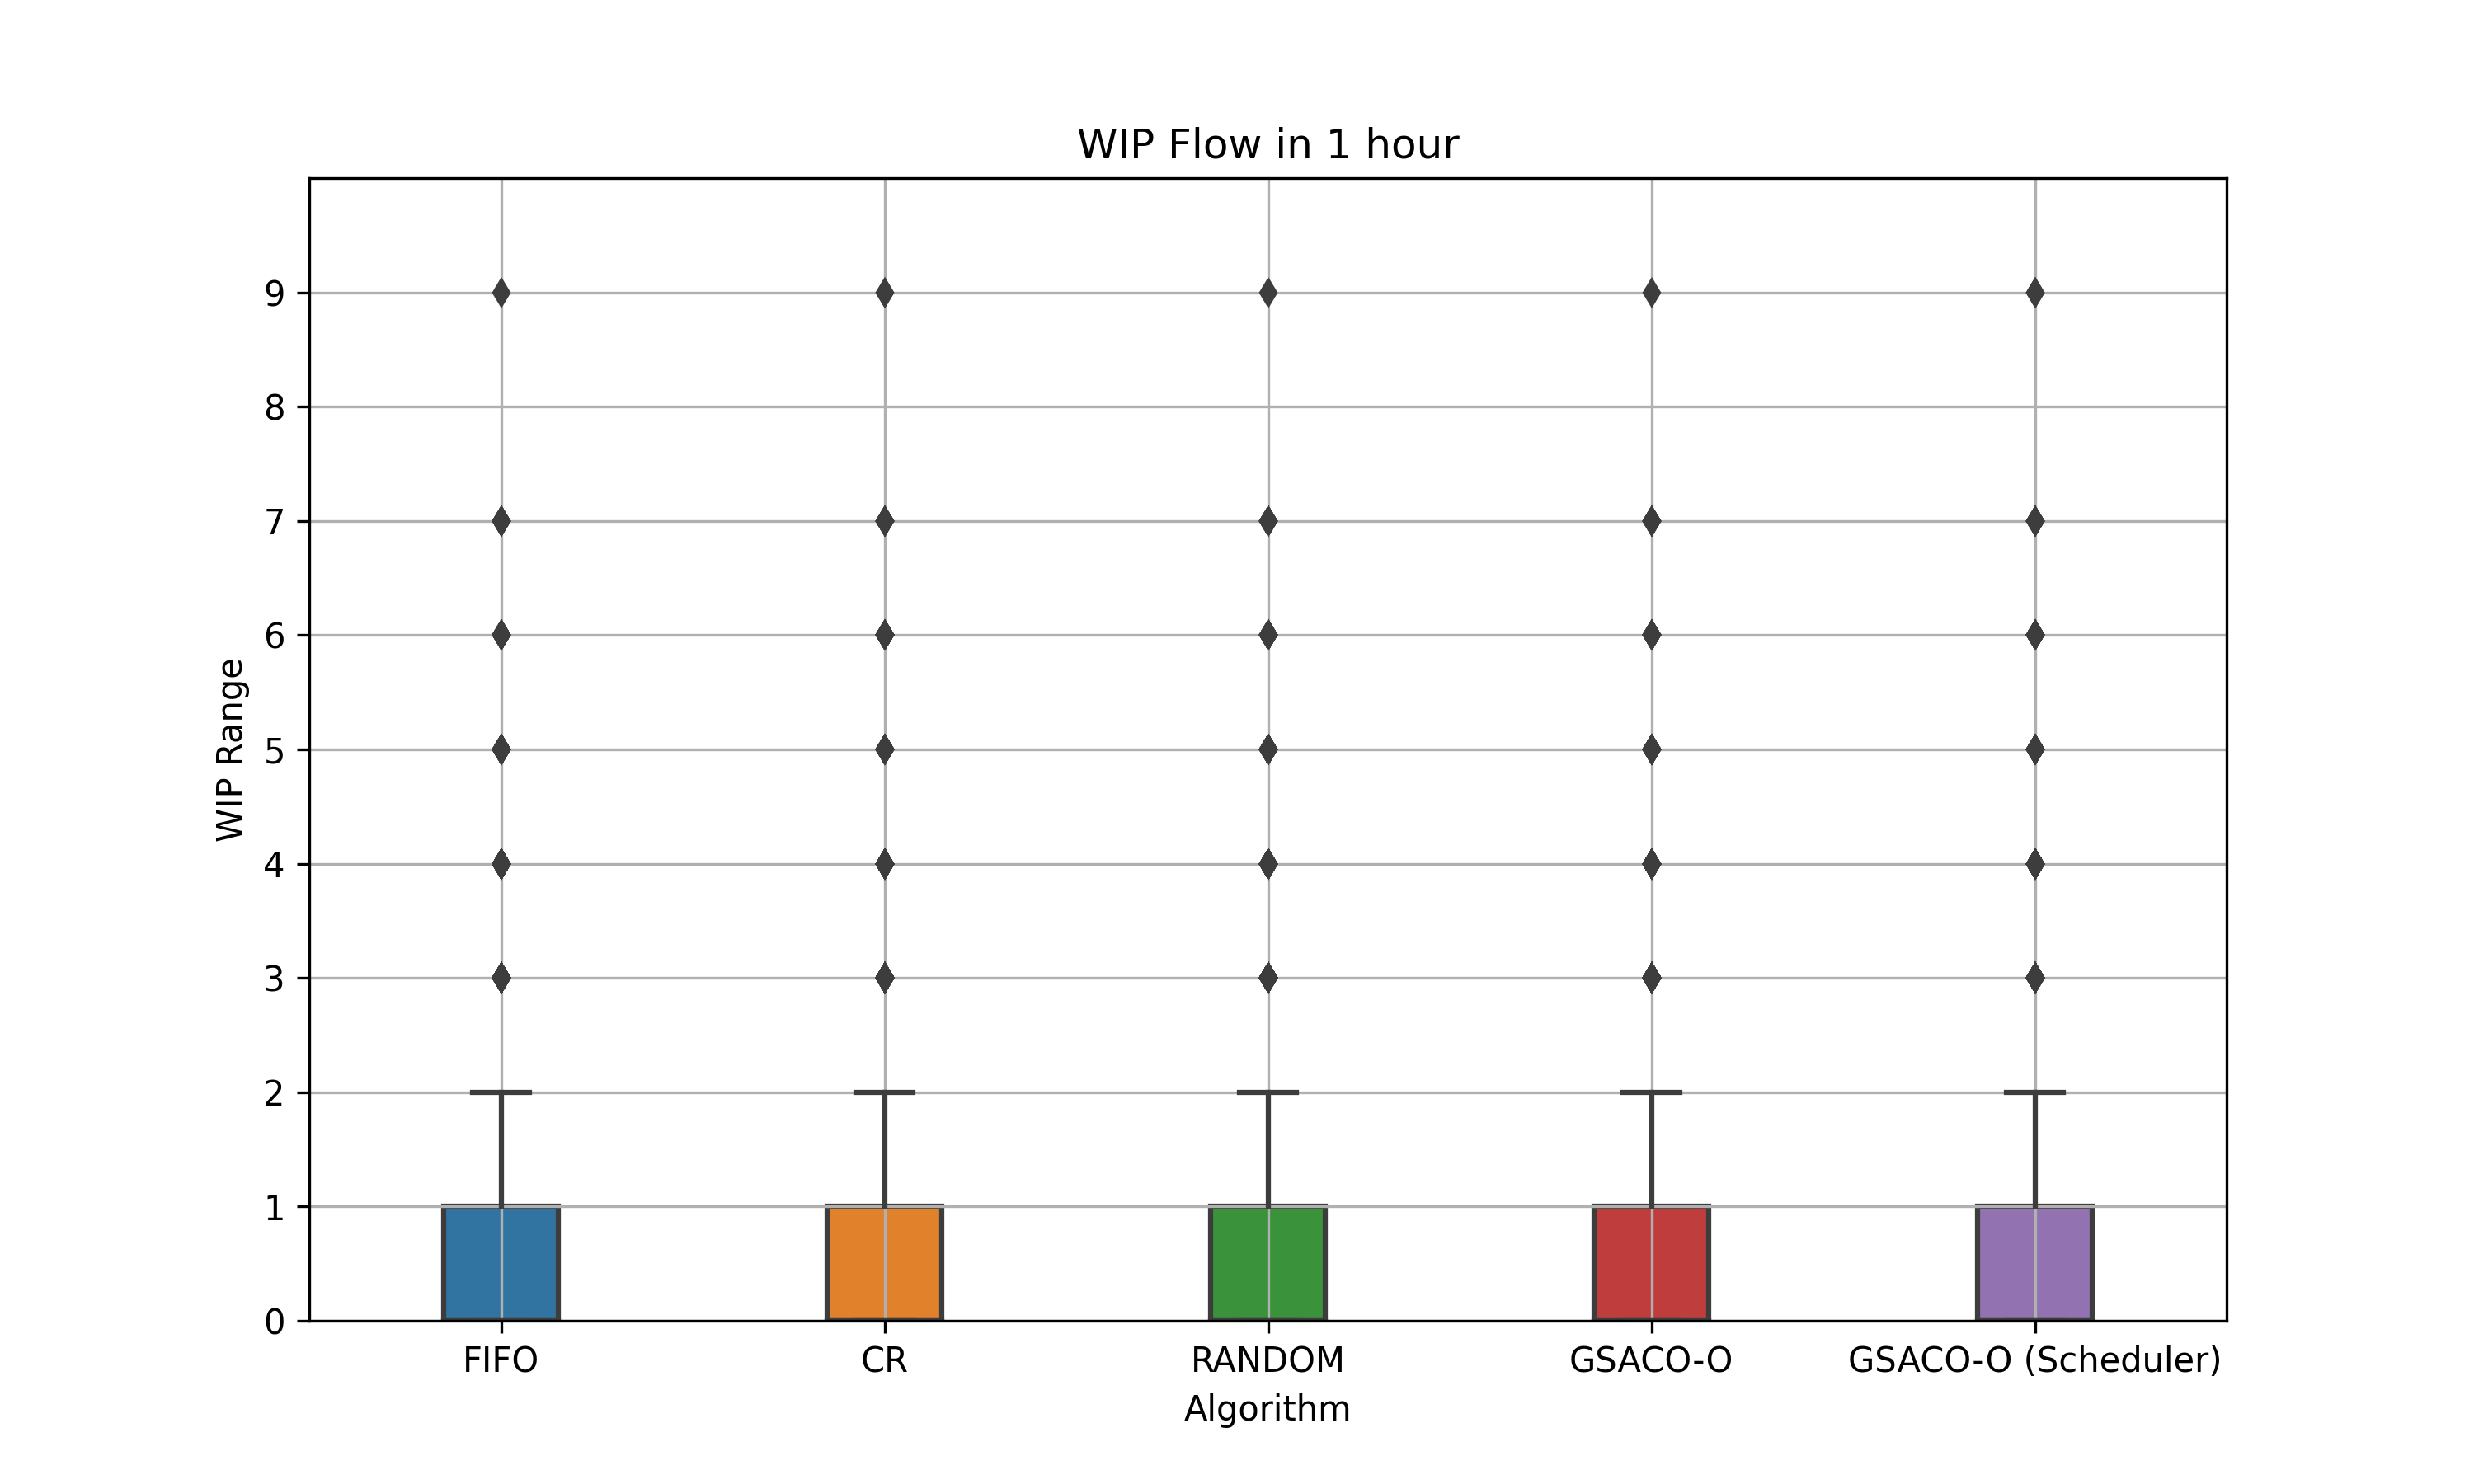
\includegraphics[width=\textwidth]{HVLM/new_period_3600s.png}
		% \caption{}
		% \label{fig:p1}
	\end{subfigure}
	\hfill
	\begin{subfigure}[b]{0.32\textwidth}
		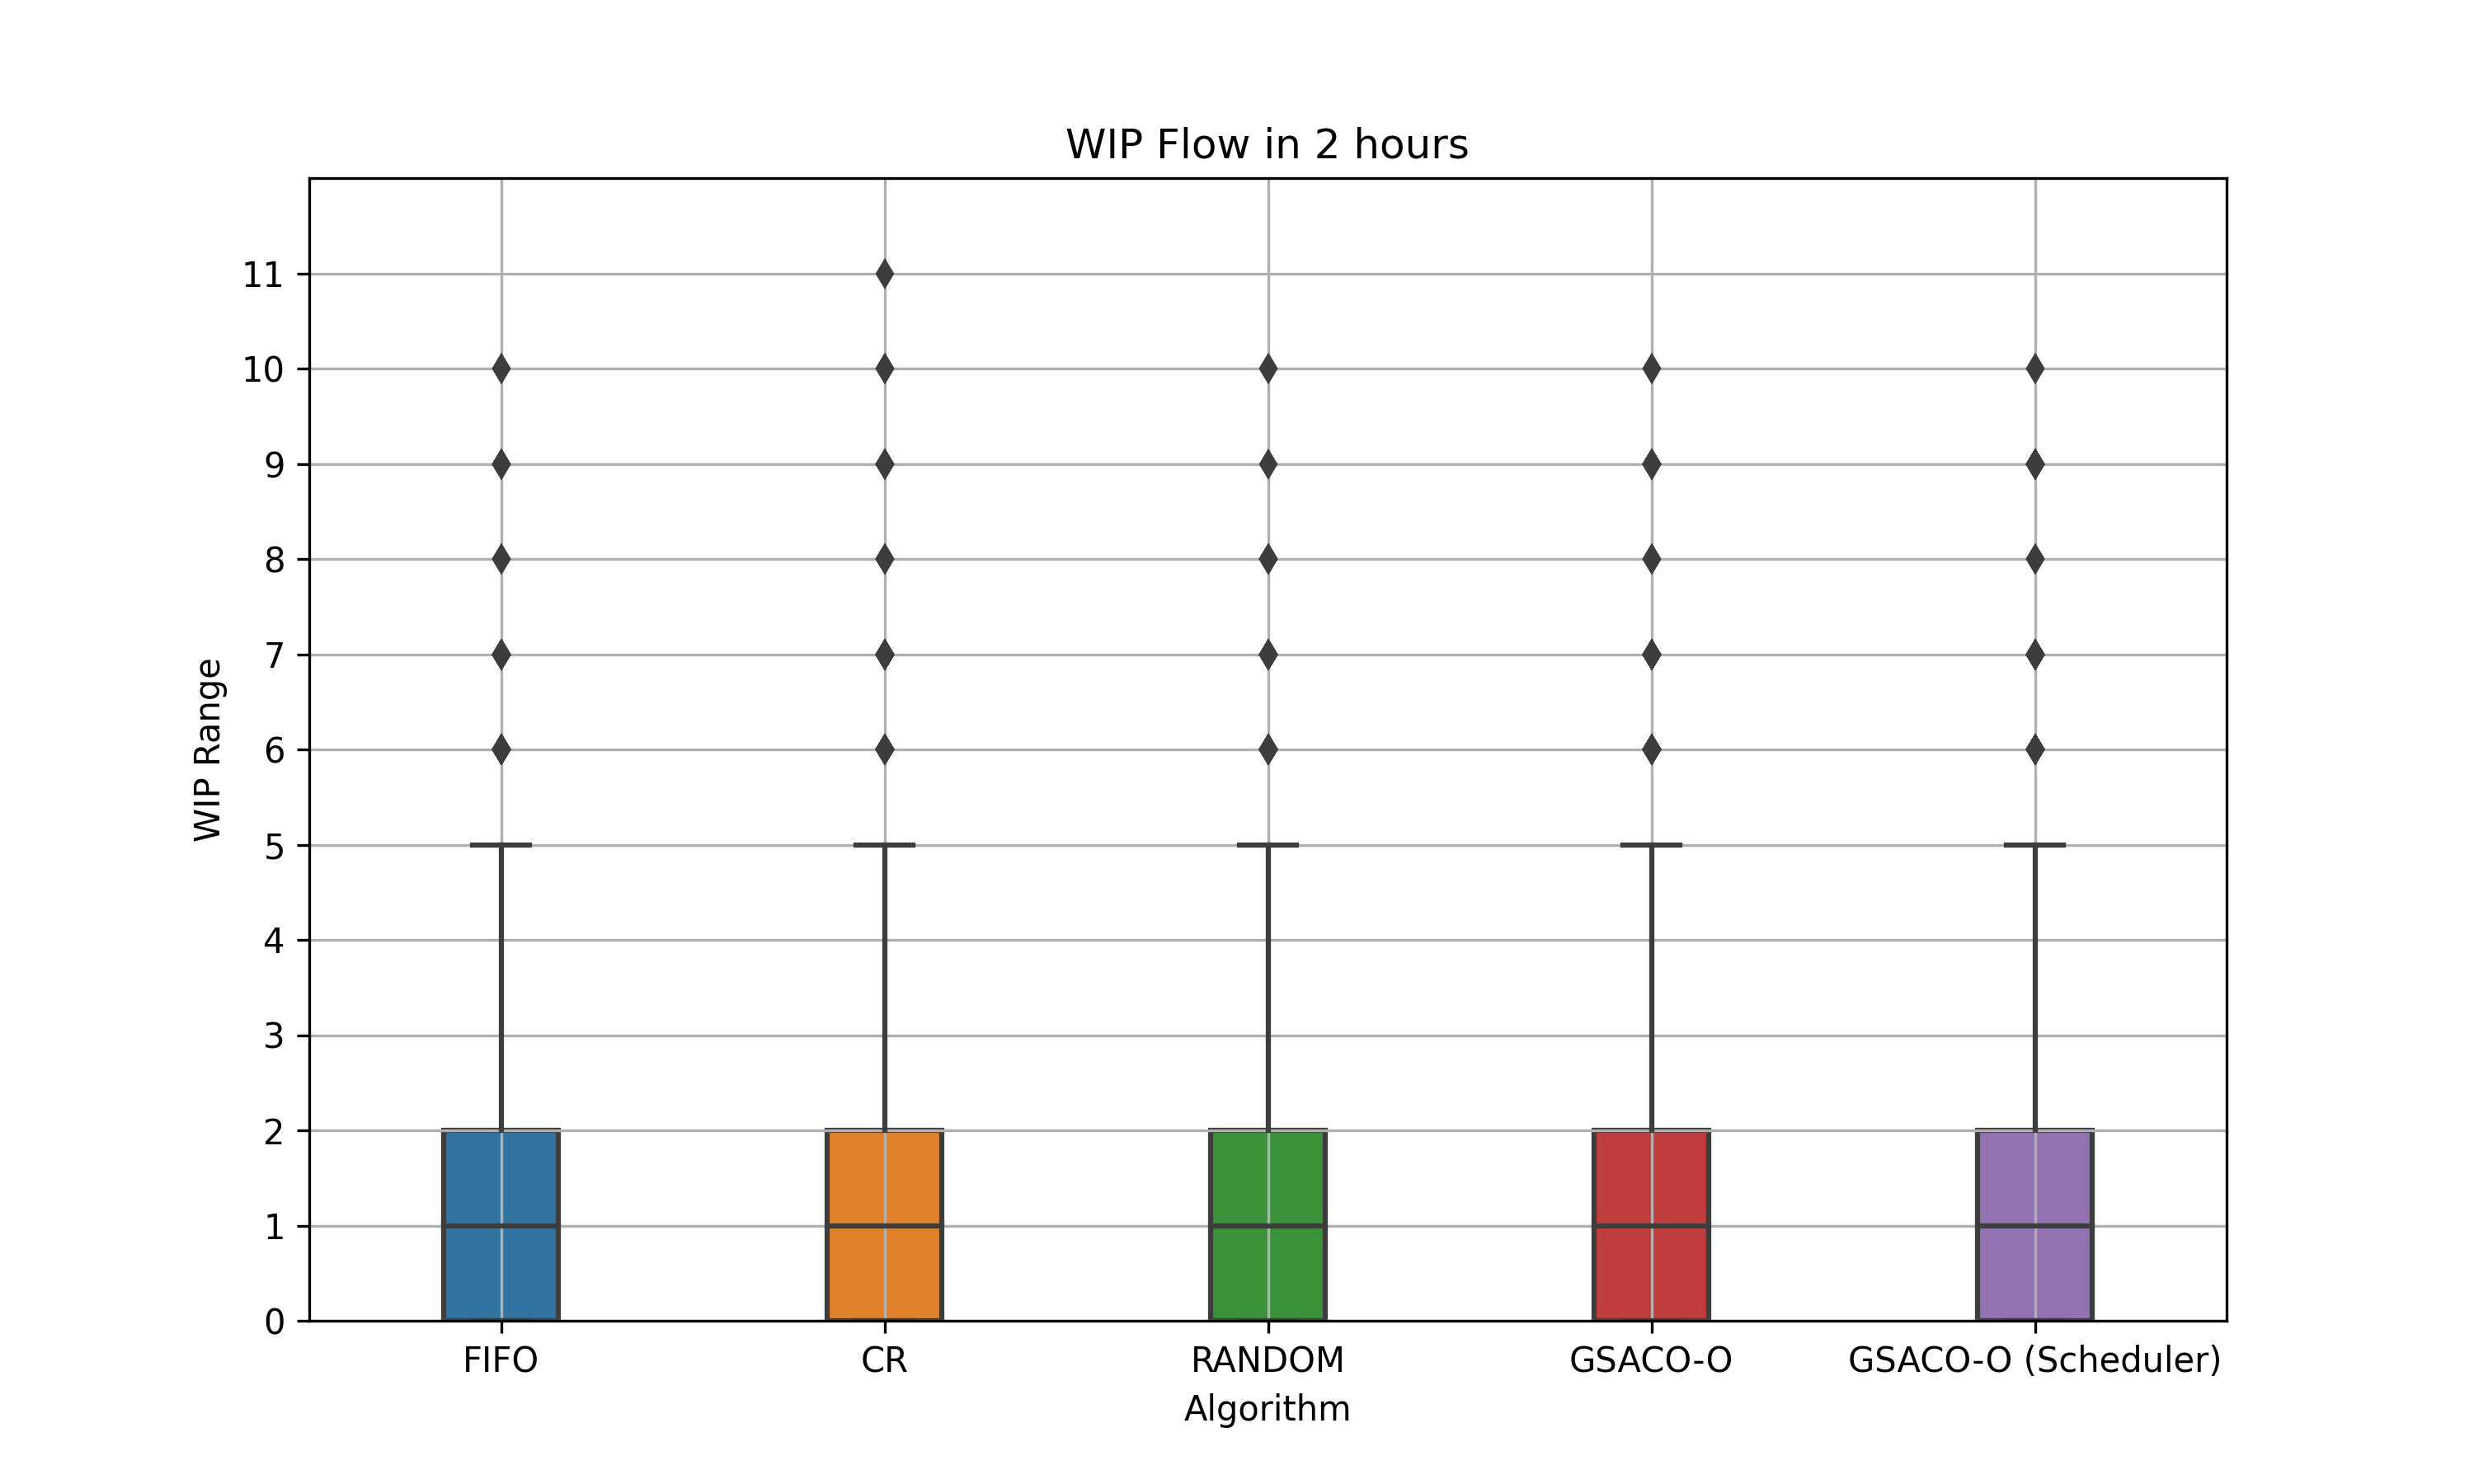
\includegraphics[width=\textwidth]{HVLM/new_period_7200s.png}
		% \caption{}
		% \label{fig:p2}
	\end{subfigure}
	\hfill
	\begin{subfigure}[b]{0.32\textwidth}
		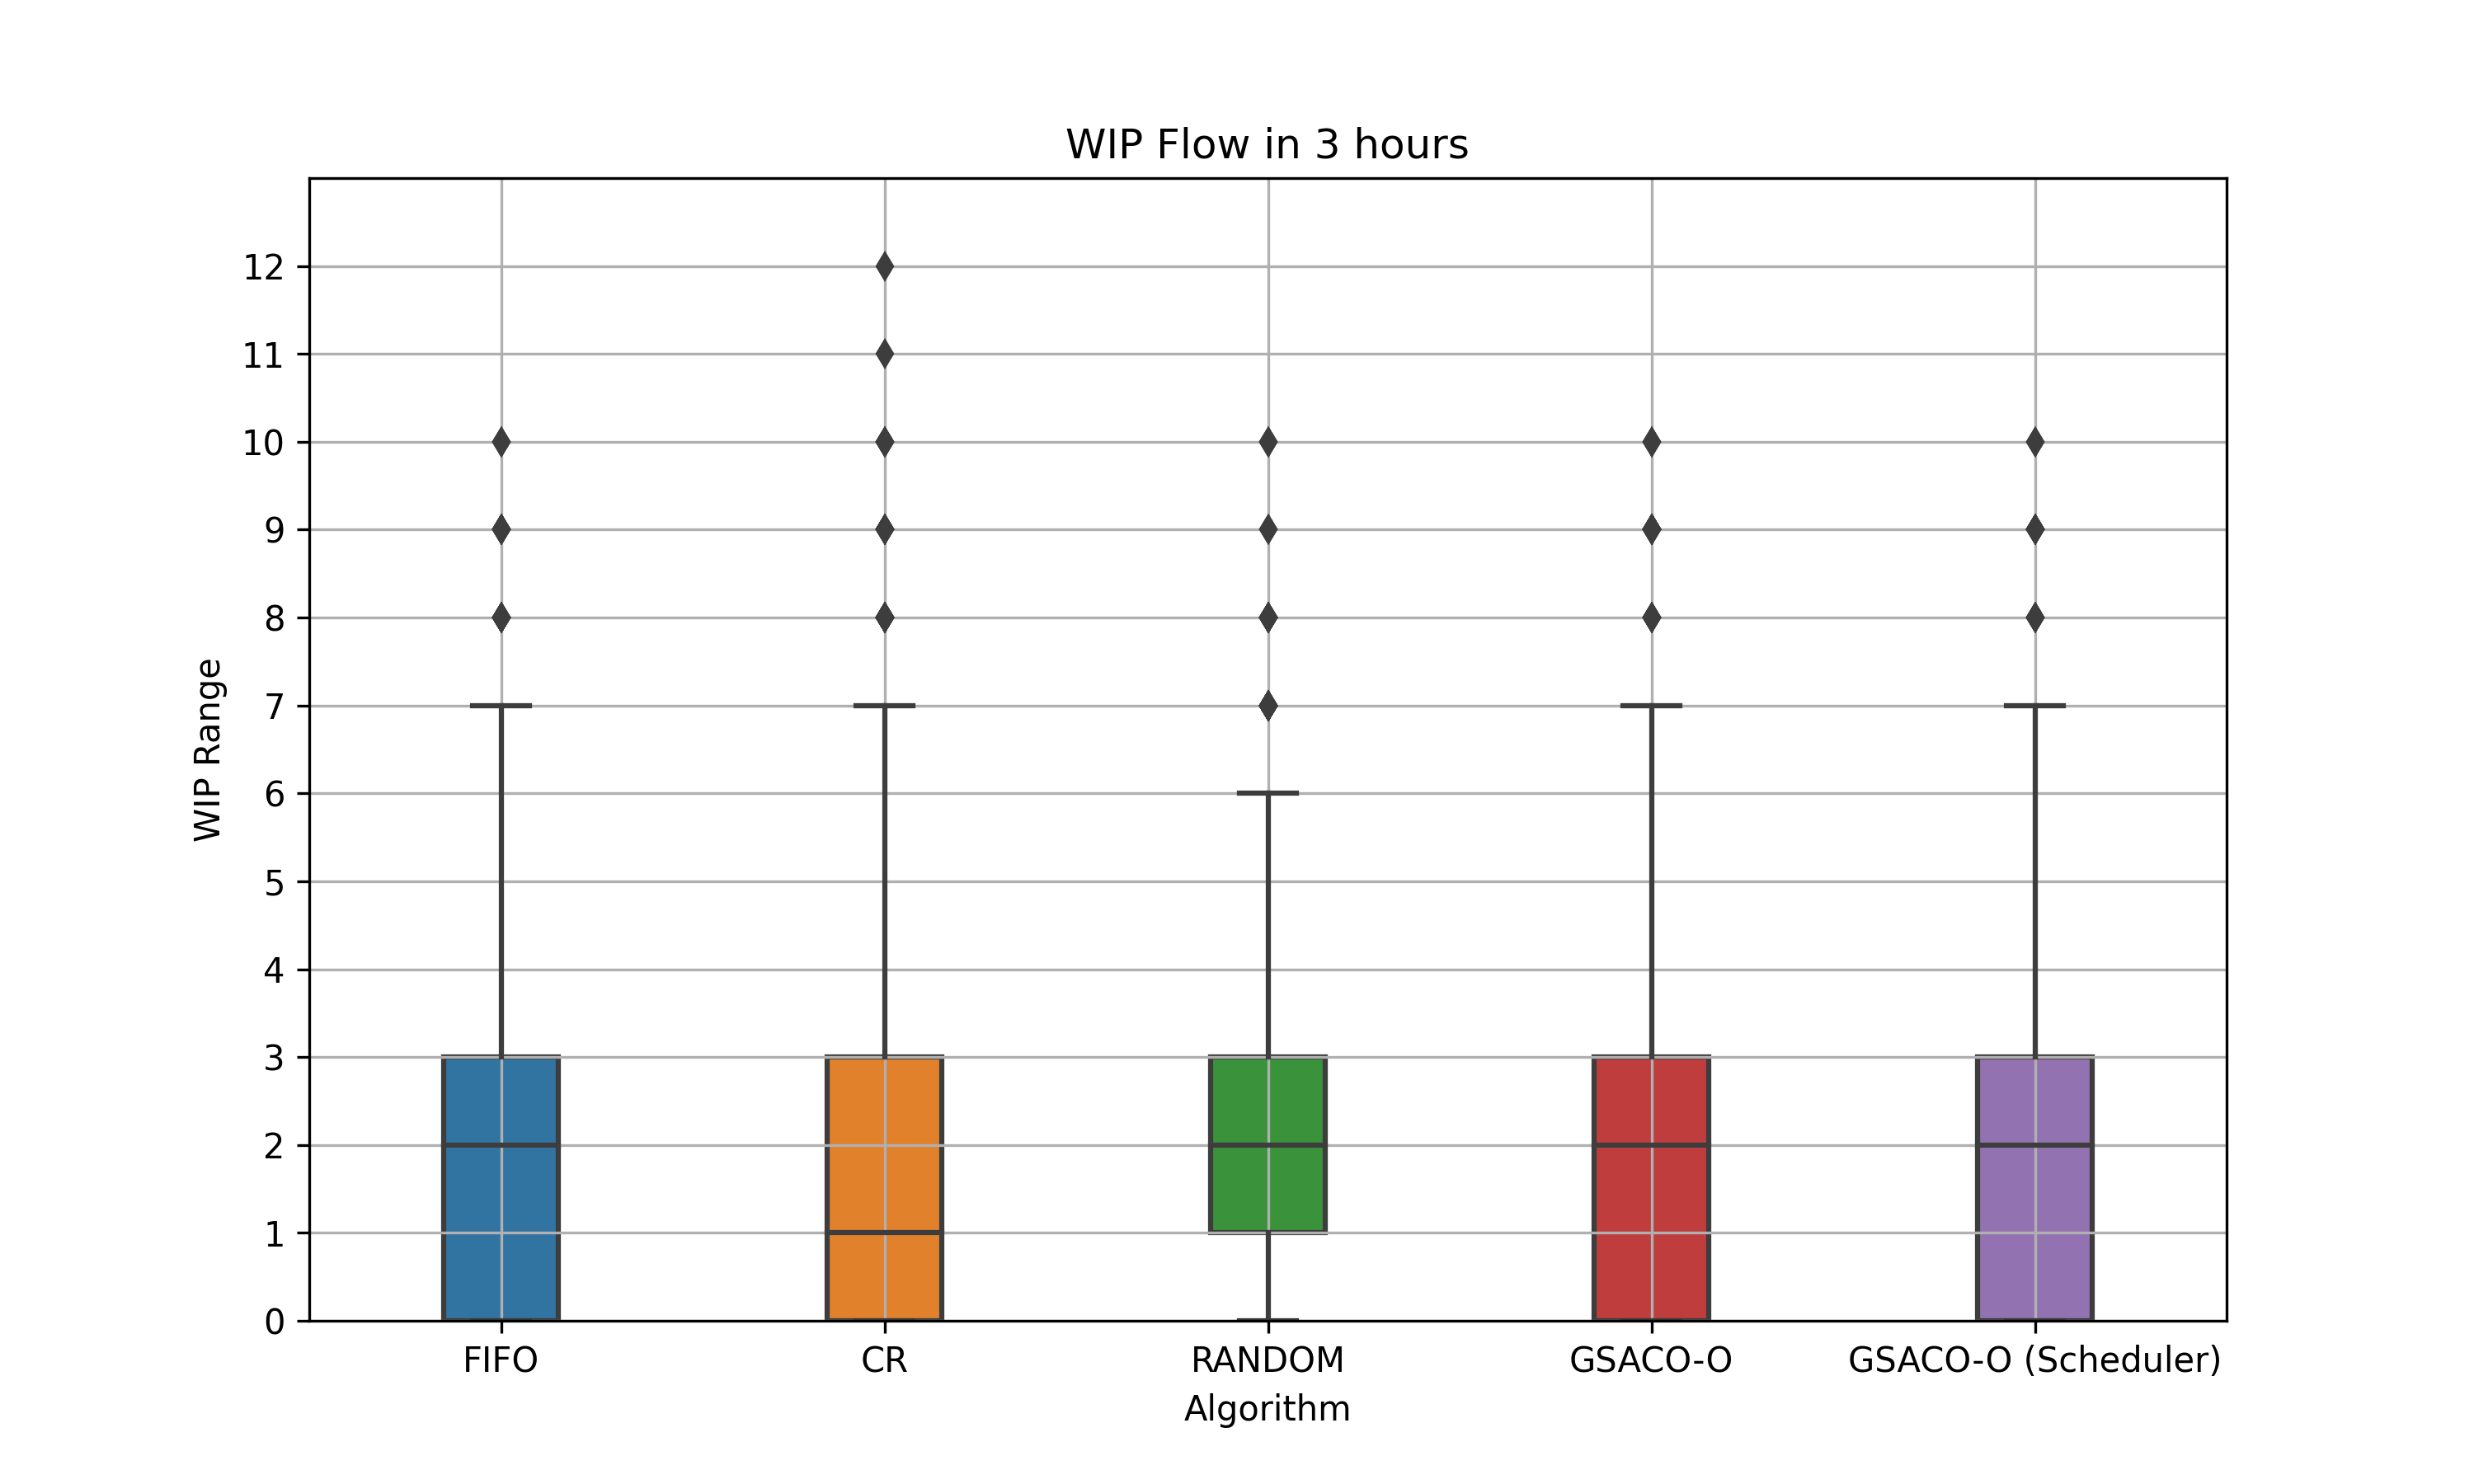
\includegraphics[width=\textwidth]{HVLM/new_period_10800s.png}
		% \caption{}
		% \label{fig:p3}
	\end{subfigure}
	
	\begin{subfigure}[b]{0.32\textwidth}
		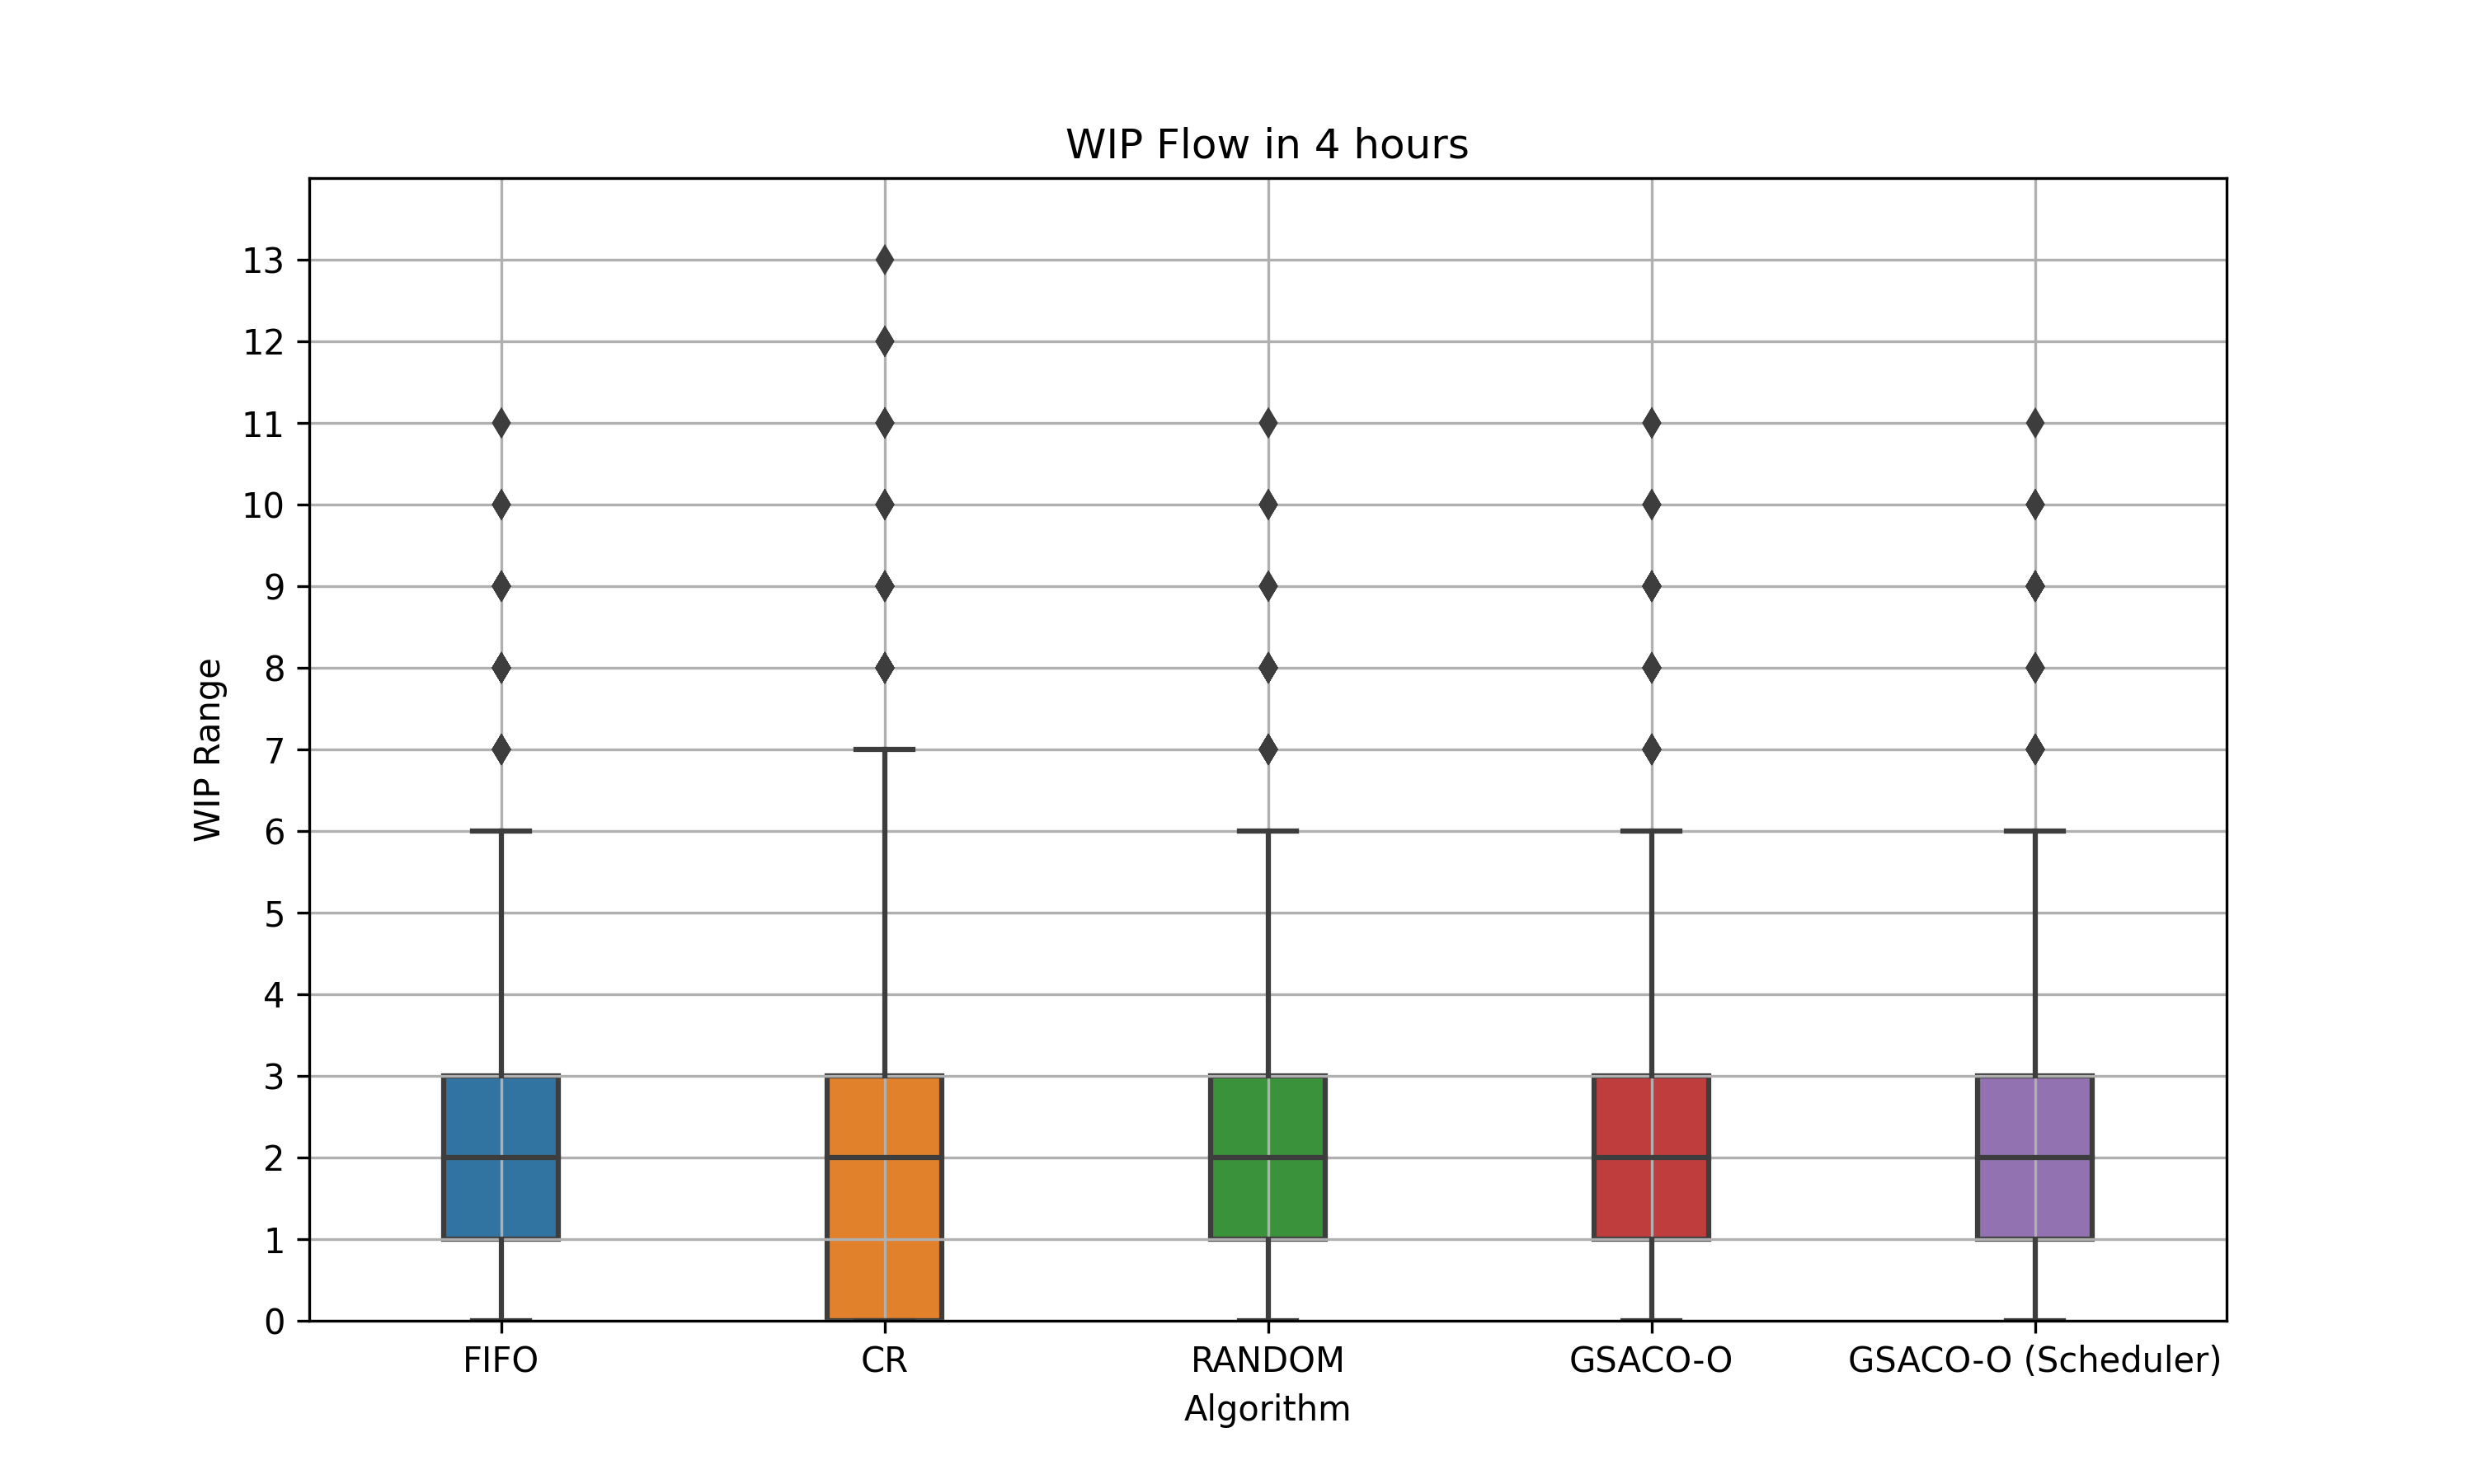
\includegraphics[width=\textwidth]{HVLM/new_period_14400s.png}
		% \caption{}
		% \label{fig:p4}
	\end{subfigure}
	\hfill
	\begin{subfigure}[b]{0.32\textwidth}
		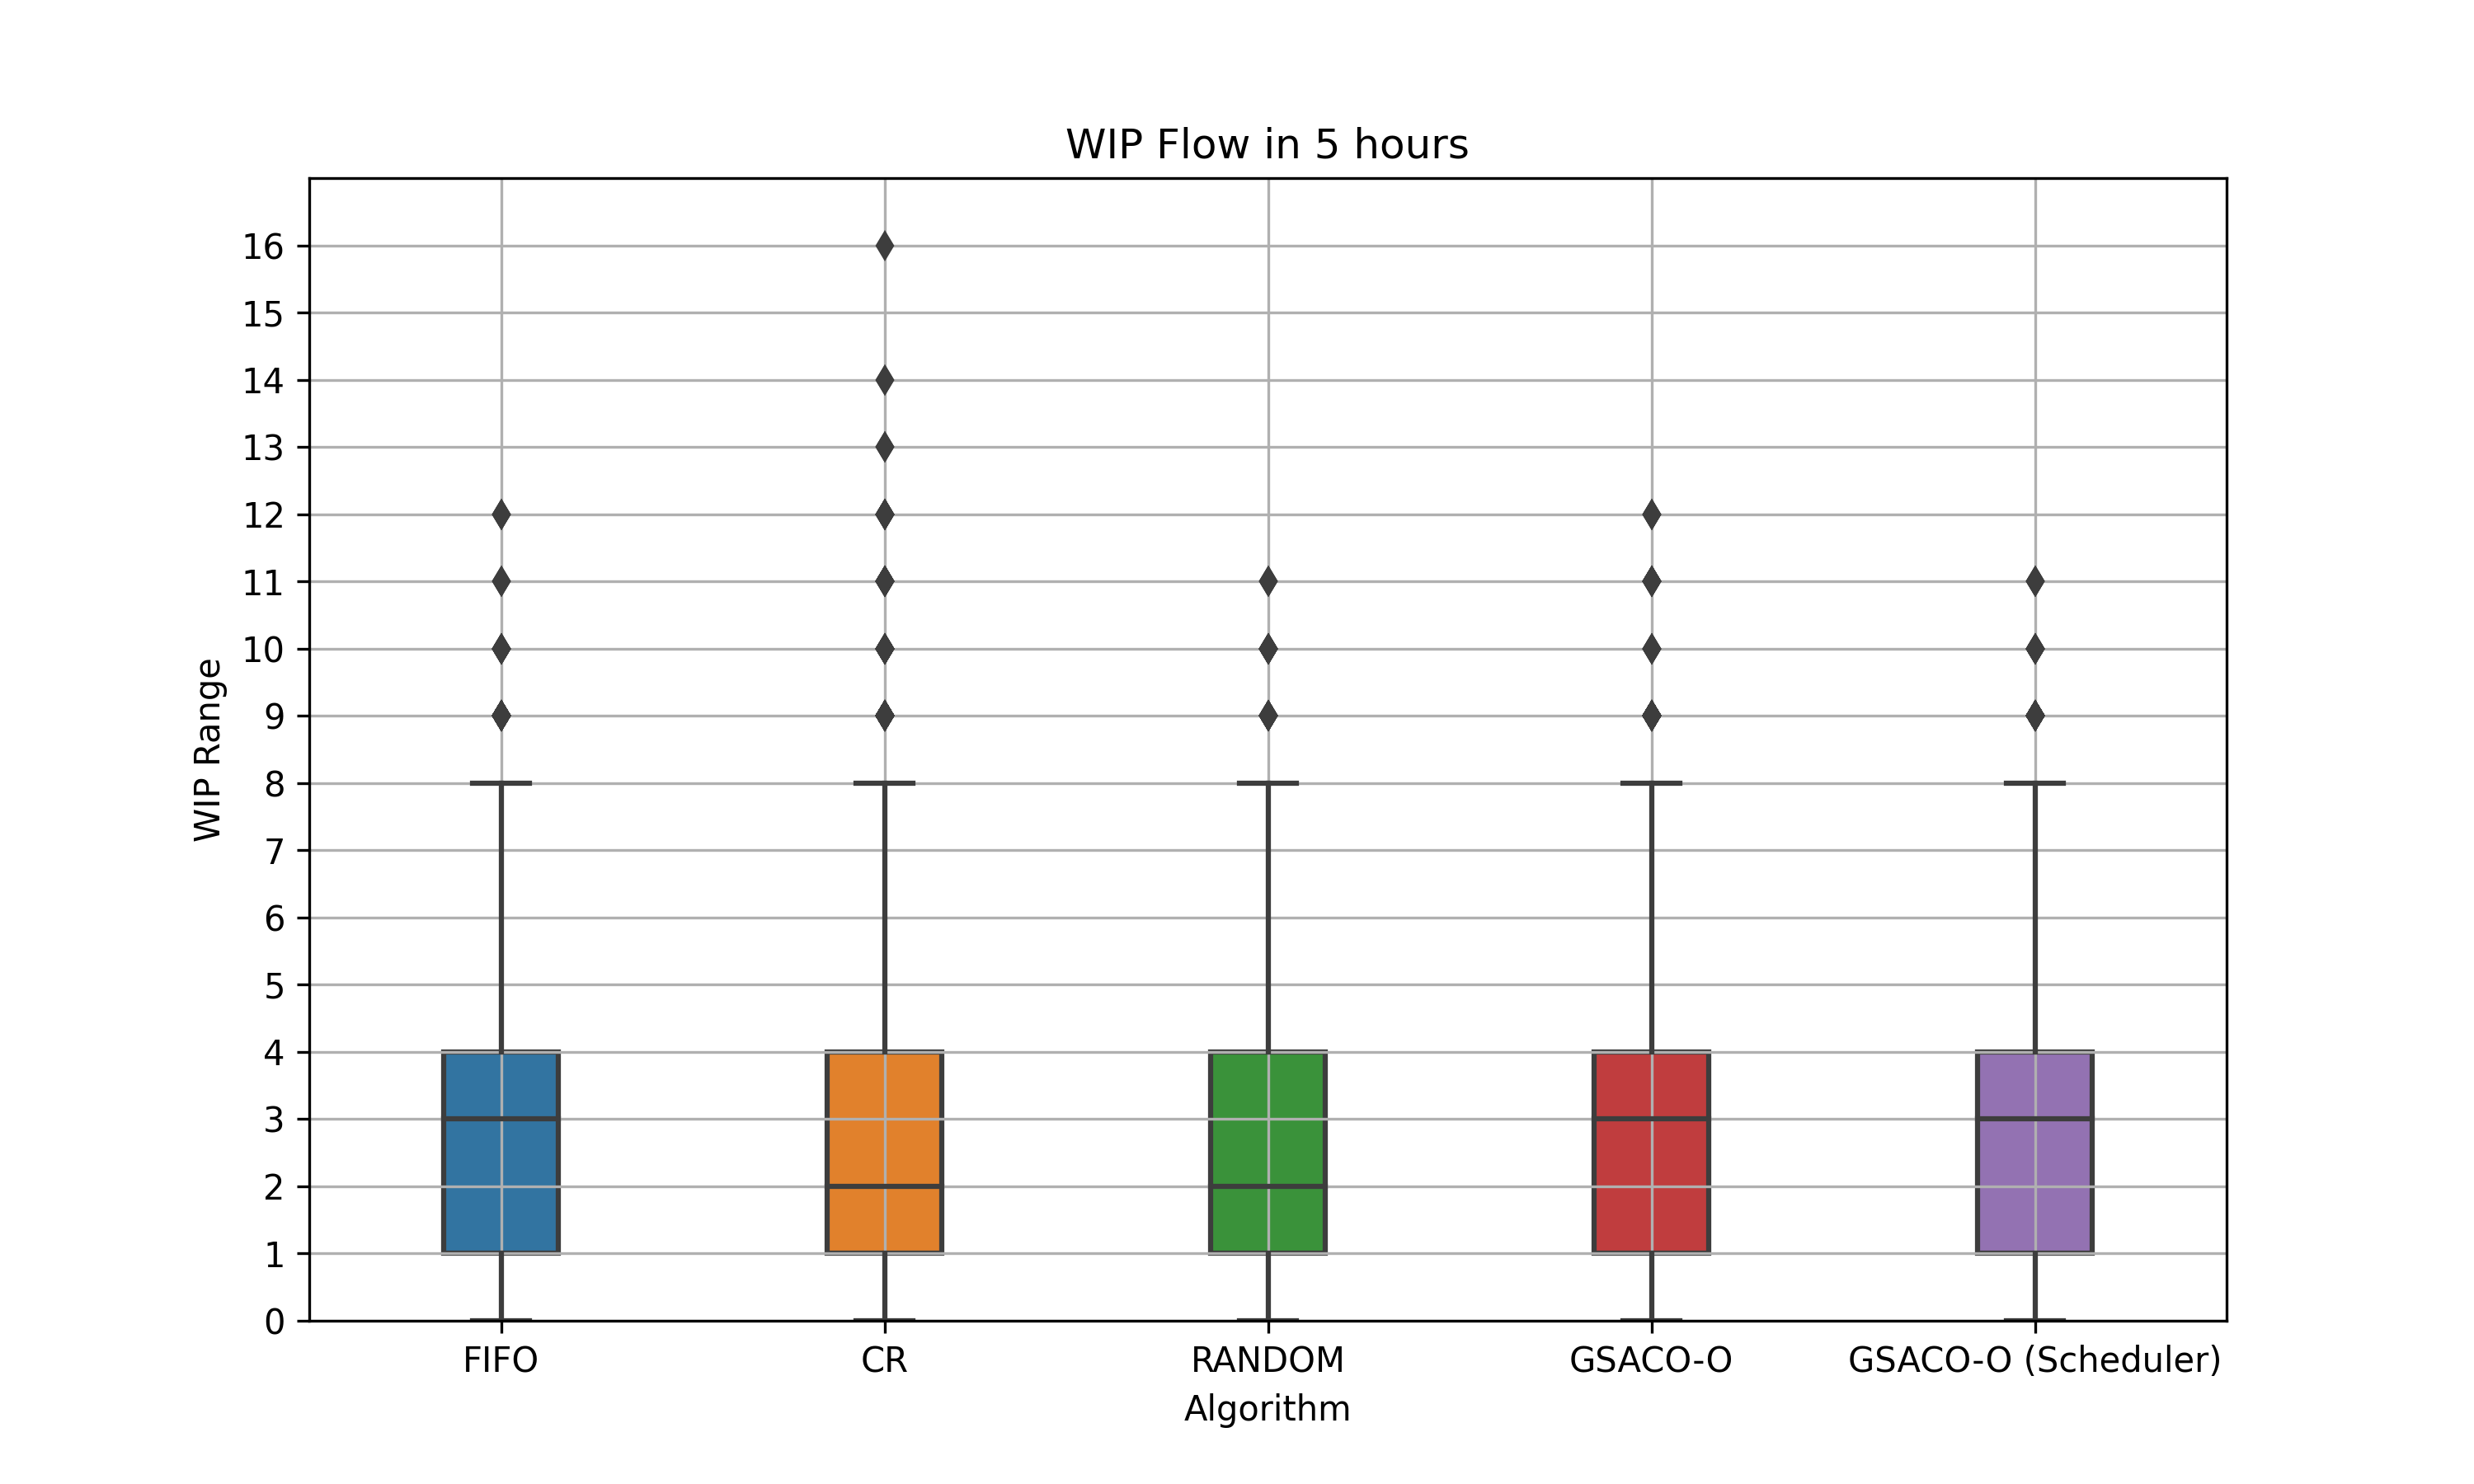
\includegraphics[width=\textwidth]{HVLM/new_period_18000s.png}
		% \caption{}
		% \label{fig:p5}
	\end{subfigure}
	\hfill
	\begin{subfigure}[b]{0.32\textwidth}
		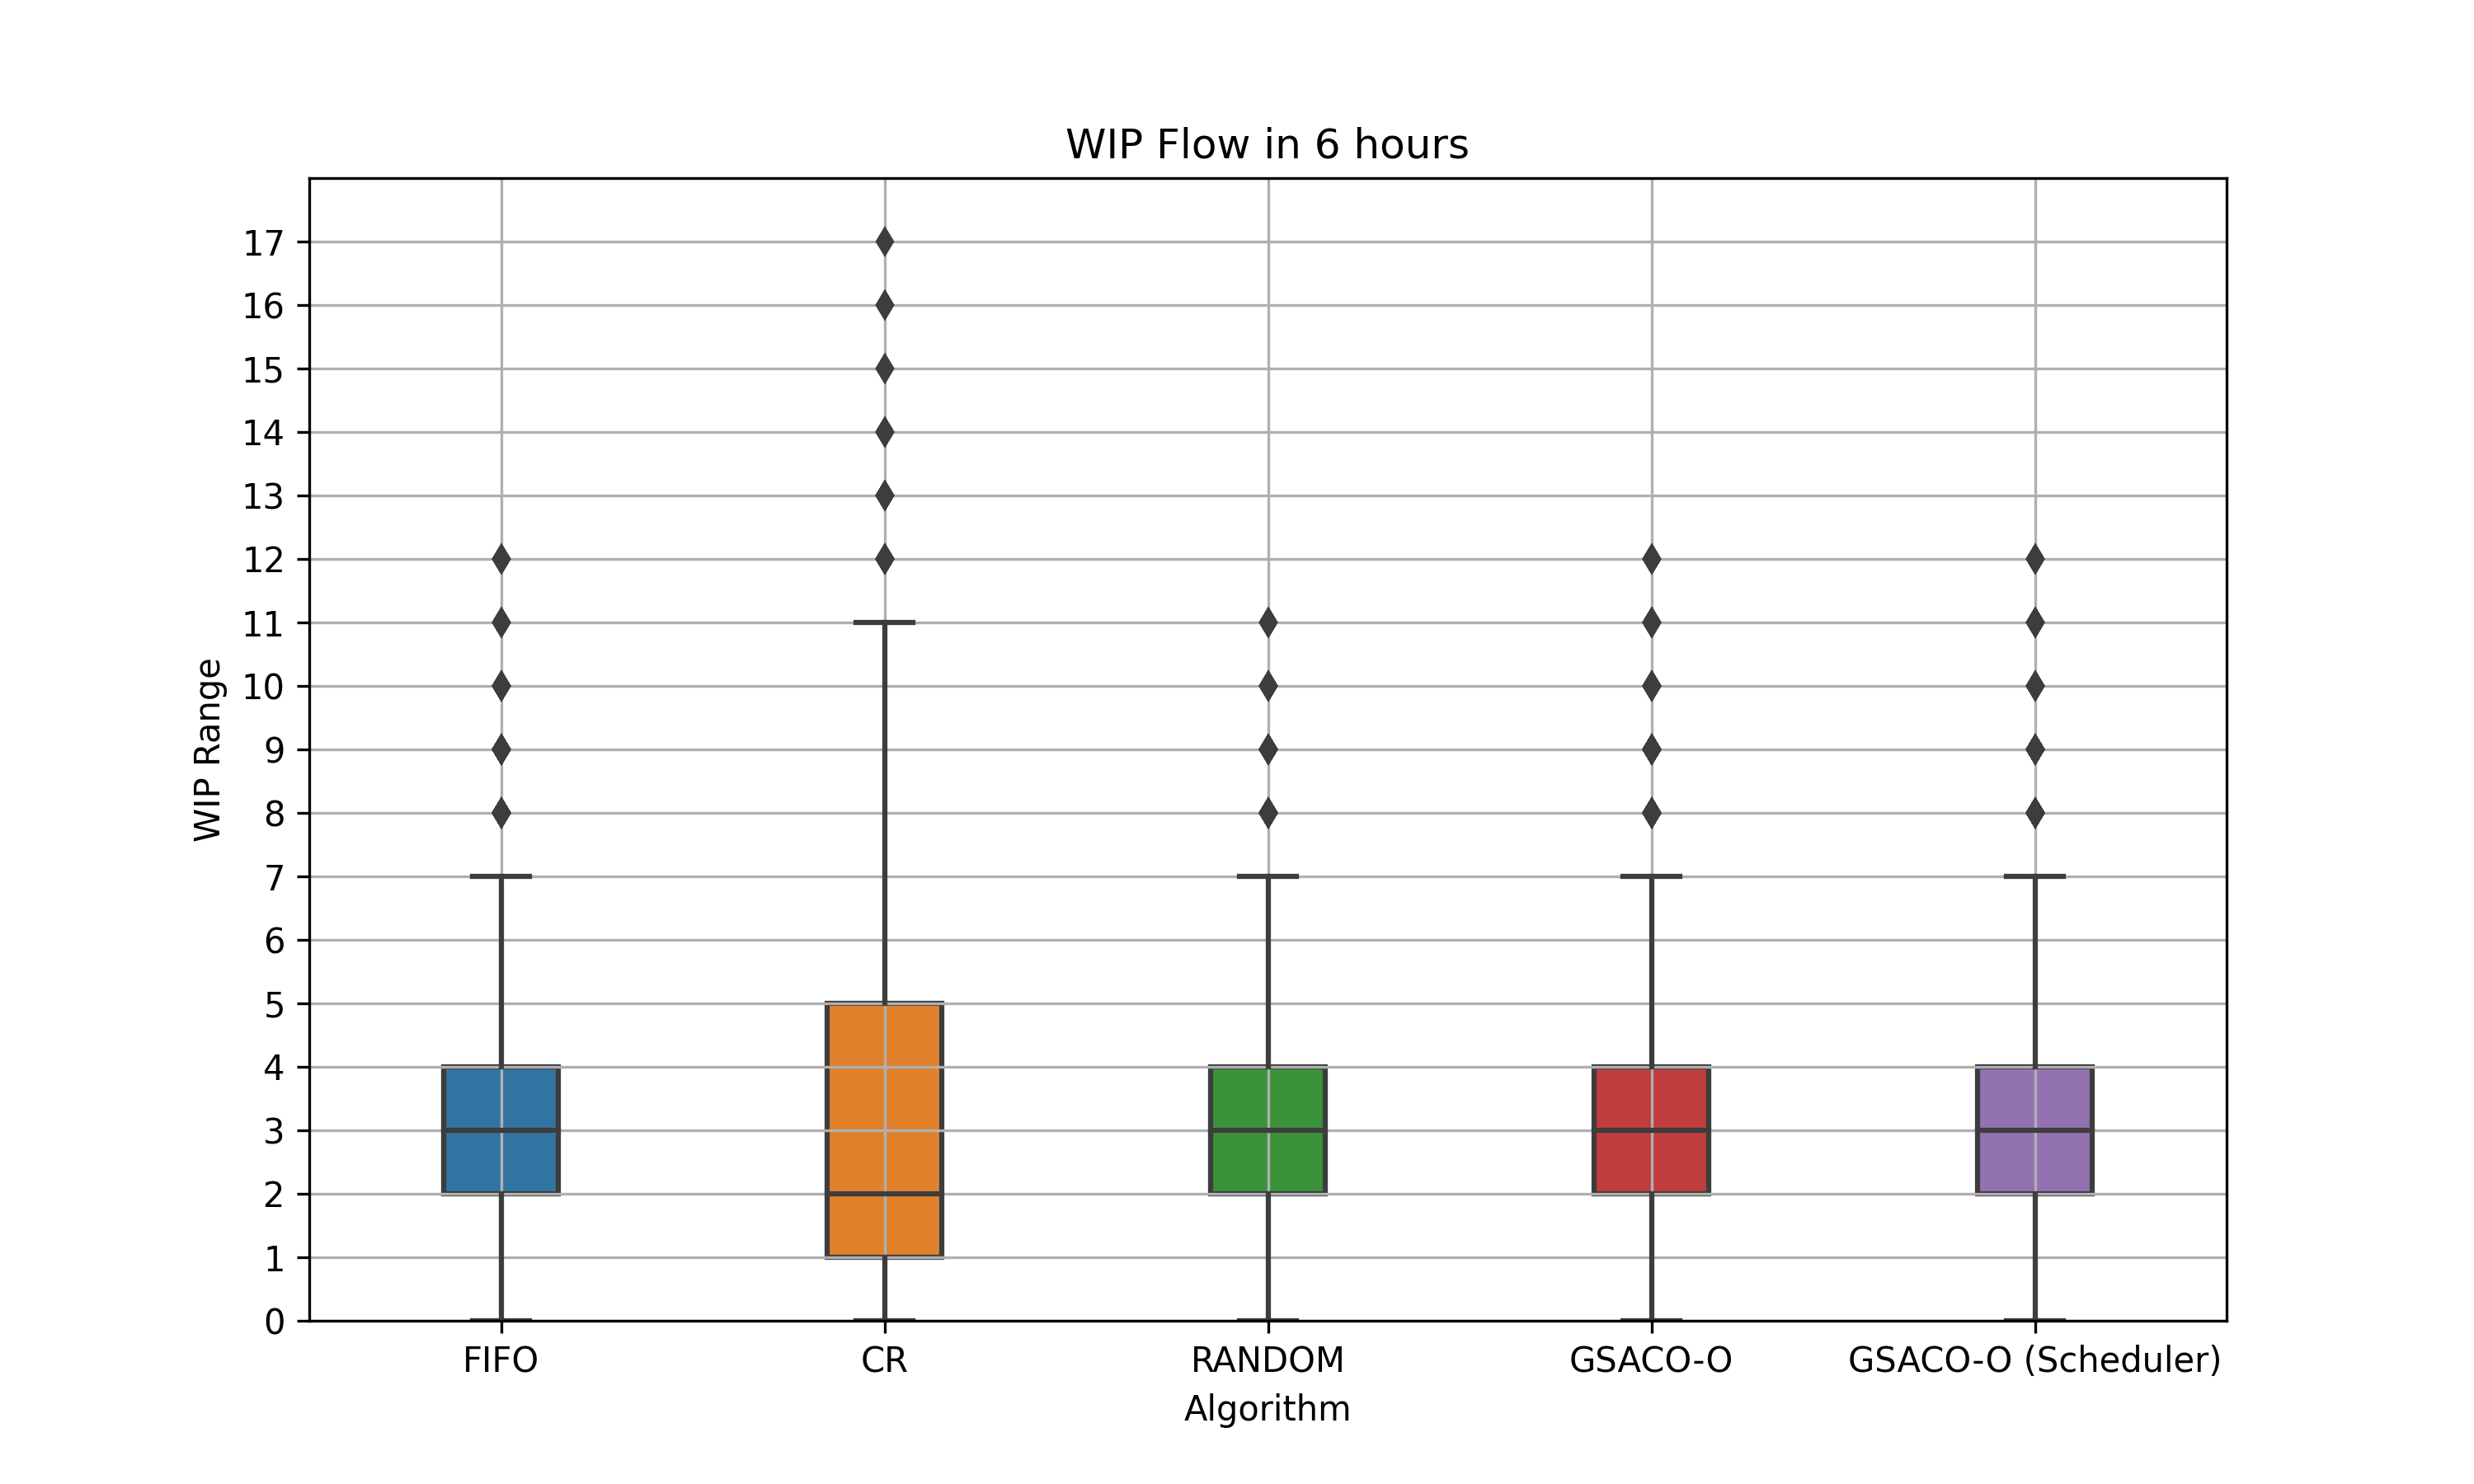
\includegraphics[width=\textwidth]{HVLM/new_period_21600s.png}
		% \caption{}
		% \label{fig:p6}
	\end{subfigure}
	\caption{WIP flow for HV/LM}
	\label{fig:wip-flows-HVLM}
\end{figure}

Similarly, the plots in Figure~\ref{fig:wip-flows-HVLM} illustrate the WIP flow for the HV/LM scenario. The FIFO dispatcher maintains a narrow interquartile range (IQR) and a relatively low WIP count in comparison to other dispatchers.
Even at 6 hours, FIFO’s WIP values are less dispersed than other algorithms, indicating a conservative and stable approach in managing WIP.
The CR dispatcher shows a slightly wider IQR than FIFO, especially noticeable in the 5th and 6th hour plots.
The RANDOM dispatcher has a consistent distribution similar to FIFO. Its WIP values increase consistently across longer planning hours, suggesting a flexible approach that does not tightly control WIP levels and makes it less predictable.
GSACO-O, when used as a dispatcher, shows a stable and controlled WIP range similar to FIFO and CR but with some incremental flexibility.
Across the time periods, GSACO-O maintains a low median and narrow IQR, suggesting an efficient handling of WIP without significant spikes. GSACO-O as a scheduler demonstrates similar behavior to its dispatcher, with low variability in WIP values.

In conclusion, the comparative analysis across different dispatching algorithms (FIFO, CR, RANDOM, GSACO-O as dispatcher, and GSACO-O as scheduler) reveals distinct characteristics in WIP handling as planning horizons extend from 1 to 6 hours.
GSACO-O, whether used as a dispatcher or scheduler, consistently demonstrates robust performance with stable WIP ranges and limited outliers, suggesting a reliable choice for applications requiring predictability in WIP levels. FIFO and CR also show controlled WIP distributions but with slightly more variability in extended periods, indicating that while they maintain order, they might face occasional increases in WIP as time progresses. RANDOM, by contrast, allows more variability, with a slightly wider IQR and an increasing number of outliers in longer horizons, which reflects a more flexible but less controlled approach to WIP management.
As planning horizons extend, all algorithms experience a rise in WIP counts and outliers, highlighting the impact of prolonged operational periods on workload variability. For scenarios prioritizing stability and predictability, GSACO-O and FIFO emerge as preferred choices.

Additionally, if WIP levels remain consistent across dispatching strategies, using a scheduler like GSACO-O could be computationally expensive without significant benefit in WIP performance. In such cases, opting for a dispatcher approach rather than a scheduler could reduce computational overhead while achieving similar WIP outcomes. These insights can guide the selection of dispatching and scheduling algorithms in settings where managing WIP levels is crucial to operational efficiency and workflow stability, with computational cost considerations also taken into account.



















\section{Conclusion}
\label{sec:conclusion}

Modern semiconductor fabs are highly complex and dynamic production
environments, whose efficient operation by means of automated scheduling
and control systems constitutes a pressing research challenge.
In this work, we model the production processes of large-scale
semiconductor fabs in terms of the well-known FJSSP.
In contrast to classical FJSSP benchmarks,
this leads to large-scale scheduling problems,
even if short planning horizons cover only a fraction of the long
production routes with hundreds of operations.
The resulting size and complexity of large-scale SMSP instances
exceed the capabilities of common FJSSP solving methods.
In our previous work \cite{Ali2024}, we showed the scalability of our proposed approach. 
We thus proposed the enhance variant of our previous GSACO algorithm, GSACO-O for optimizing operational troughput over different planning horizons.

We evaluated our scheduler through simulation as a dispatcher and compared the performance with traditional dispatching rules. In future work, we aim to evaluate our enhanced dispatching rule under different machine breakdown scenarios. 
Our second target of future work concerns hyperparameter tuning of GSACO-O parameetrs using machine learning.

We evaluated our scheduler by simulating it as a dispatcher and comparing its performance with traditional dispatching rules. The results indicate that our approach can potentially streamline operations. For future work, we plan to assess the effectiveness of our enhanced dispatching rule under various machine breakdown scenarios, which will provide insights into its resilience and adaptability in dynamic environments.
Additionally, we aim to explore hyperparameter tuning of GSACO-O parameters through machine learning techniques to further optimize performance. Leveraging machine learning could help us identify optimal configurations more efficiently, enhancing the scheduler's responsiveness and adaptability to different manufacturing setups.

\section*{Acknowledgments}
This work has been funded by the FFG project 894072 (SwarmIn).
We are grateful to the anonymous reviewers for constructive 
comments that helped to improve the presentation of this paper.




%
% ---- Bibliography ----
%
% BibTeX users should specify bibliography style 'splncs04'.
% References will then be sorted and formatted in the correct style.
%
% \bibliographystyle{splncs04}
% \bibliography{mybibliography}
%
\begin{thebibliography}{8}
	\bibitem{kopp2020smt2020}
	Kopp, D., Hassoun, M., Kalir, A., Mönch, L.: SMT2020—a semiconductor manufacturing testbed. IEEE Transactions on Semiconductor Manufacturing 33(4):522–531 (2020)
	
	\bibitem{Hopp2011}
	Hopp, W. J., Spearman, M. L.: Factory physics. Waveland Press. (2011)
	
	\bibitem{Uzsoy1992}
	Uzsoy, R., Lee, C. Y., Martin-Vega, L. A.: A review of production planning and scheduling models in the semiconductor industry part I: system characteristics, performance evaluation and production planning. IIE transactions, 24(4), 47-60 (1992)
	
	\bibitem{schumann2022scheduling}
	Pinedo, M. L.: Scheduling: theory, algorithms, and systems. 6th edn. Springer (2022) 
	
	\bibitem{May2006}
	May, G. S., Spanos, C. J.: Fundamentals of semiconductor manufacturing and process control. John Wiley \& Sons. (2006)
	
	\bibitem{Mönch2011}
	Mönch, L., Fowler, J. W., Dauzère-Pérès, S., Mason, S. J., Rose, O.: A survey of problems, solution techniques, and future challenges in scheduling semiconductor manufacturing operations. Journal of scheduling, 14, 583-599. (2011)
	
	\bibitem{Ali2024}
	Ali, R., Qaiser, S., El-Kholany, M. M., Eftekhari, P., Gebser, M., Leitner, S., Friedrich, G. A Greedy Search Based Ant Colony Optimization Algorithm for Large-Scale Semiconductor Production. In Proceedings of the 14th International Conference on Simulation and Modeling Methodologies, Technologies and Applications (SIMULTECH 2024), pages 138-149. (2024)
	
	\bibitem{Dorigo2019}
	Dorigo, M., Stützle, T.: Ant colony optimization: overview and recent advances. In Handbook of Metaheuristics, pages 311–351. Springer (2019)
	
	\bibitem{Papadimitriou}
	Papadimitriou, C. H., Steiglitz, K.: Combinatorial Optimization: Algorithms and Complexity. Prentice-Hall. (1982)
	
	\bibitem{Perron2023}
	Perron, L., Didier, F., Gay, S.: The CP-SATLP
	solver (invited talk). In Proceedings of the 29th
	International Conference on Principles and Practice
	of Constraint Programming, pages 3:1–3:2. Leibniz
	International Proceedings in Informatics, (2023)
	
	\bibitem{Kovács2022}
	Kovács, B., Tassel, P., Ali, R., El-Kholany, M., Gebser, M., Seidel, G.: A customizable simulator for artificial intelligence research to schedule semiconductor fabs. In 2022 33rd Annual SEMI Advanced Semiconductor Manufacturing Conference (ASMC) (pp. 1-6). IEEE, (2022, May)
	
	\bibitem{waschneck2018deep}
	Waschneck, B., Reichstaller, A., Belzner, L., Altenmüller, T., Bauernhansl, T., Knapp, A., Kyek, A.: Deep reinforcement learning for semiconductor production scheduling. In 2018 29th annual SEMI advanced semiconductor manufacturing conference (ASMC) pp. 301-306. IEEE, (2018, April)
	
	\bibitem{leachman1996benchmarking}
	Leachman, R. C., Hodges, D. A.: Benchmarking semiconductor manufacturing. IEEE transactions on semiconductor manufacturing 9(2), 158-169 (1996)
	
	\bibitem{McKay2003}
	McKay, K. N., Wiers, V. C.: Planning, scheduling and dispatching tasks in production control. Cognition, Technology \& Work, 5, 82-93 (2003)
	
	\bibitem{chan2024situation}
	Chan, C. W.: Situation aware dispatching system for semiconductor manufacturing. (2024)


	\bibitem{ref_article1}
	Author, F.: Article title. Journal \textbf{2}(5), 99--110 (2016)
	
	\bibitem{ref_lncs1}
	Author, F., Author, S.: Title of a proceedings paper. In: Editor,
	F., Editor, S. (eds.) CONFERENCE 2016, LNCS, vol. 9999, pp. 1--13.
	Springer, Heidelberg (2016). \doi{10.10007/1234567890}
	
	\bibitem{ref_book1}
	Author, F., Author, S., Author, T.: Book title. 2nd edn. Publisher,
	Location (1999)
	
	\bibitem{ref_proc1}
	Author, A.-B.: Contribution title. In: 9th International Proceedings
	on Proceedings, pp. 1--2. Publisher, Location (2010)
	
	\bibitem{ref_url1}
	LNCS Homepage, \url{http://www.springer.com/lncs}, last accessed 2023/10/25
\end{thebibliography}
\end{document}
